\chapter{The COMPASS Experiment at CERN} 
\label{Chap::compass}
\ifpdf
\graphicspath{{Chapters/COMPASS/Figs/Raster/}{Chapters/COMPASS/Figs/PDF/}{Chapters/COMPASS/Figs/}}
\else \graphicspath{{Chapters/COMPASS/Figs/Vector/}{Chapters/COMPASS/Figs/}} \fi

The COmmon Muon Proton Apparatus for Structure and Spectroscopy (COMPASS)
experiment is a fixed target experiment at located in France in the North Area
at CERN.  COMPASS started taking data in 2002 in the same hall as earlier
Euopean Muon Collaboration (EMC), New Muon Collaboration (NMC) and Spin Muon
Collaboration (SMC) experiments.  COMPASS has studied hadron structure through
(SI)DIS, Drell-Yan and Primakoff reactions and has done hadron spectroscopy
measurements.  \par

CERN is the European Organization for Nuclear physics research. It is located
part in France and part in Switzerland and includes many experiments and
accelerators providing beam to these experiments.  The accelerator beam lines
are connected and feed beam to each other resulting in an increase in beam
momentum at each successive accelerator.  A schematic of the accelerators at
CERN is shown in Fig.~\ref{fig::CERNaccelerators} where the accelerator that
sends beam to COMPASS is the Super Proton Synchrotron (SPS). \par

\begin{figure}[h!t]
  \centering
  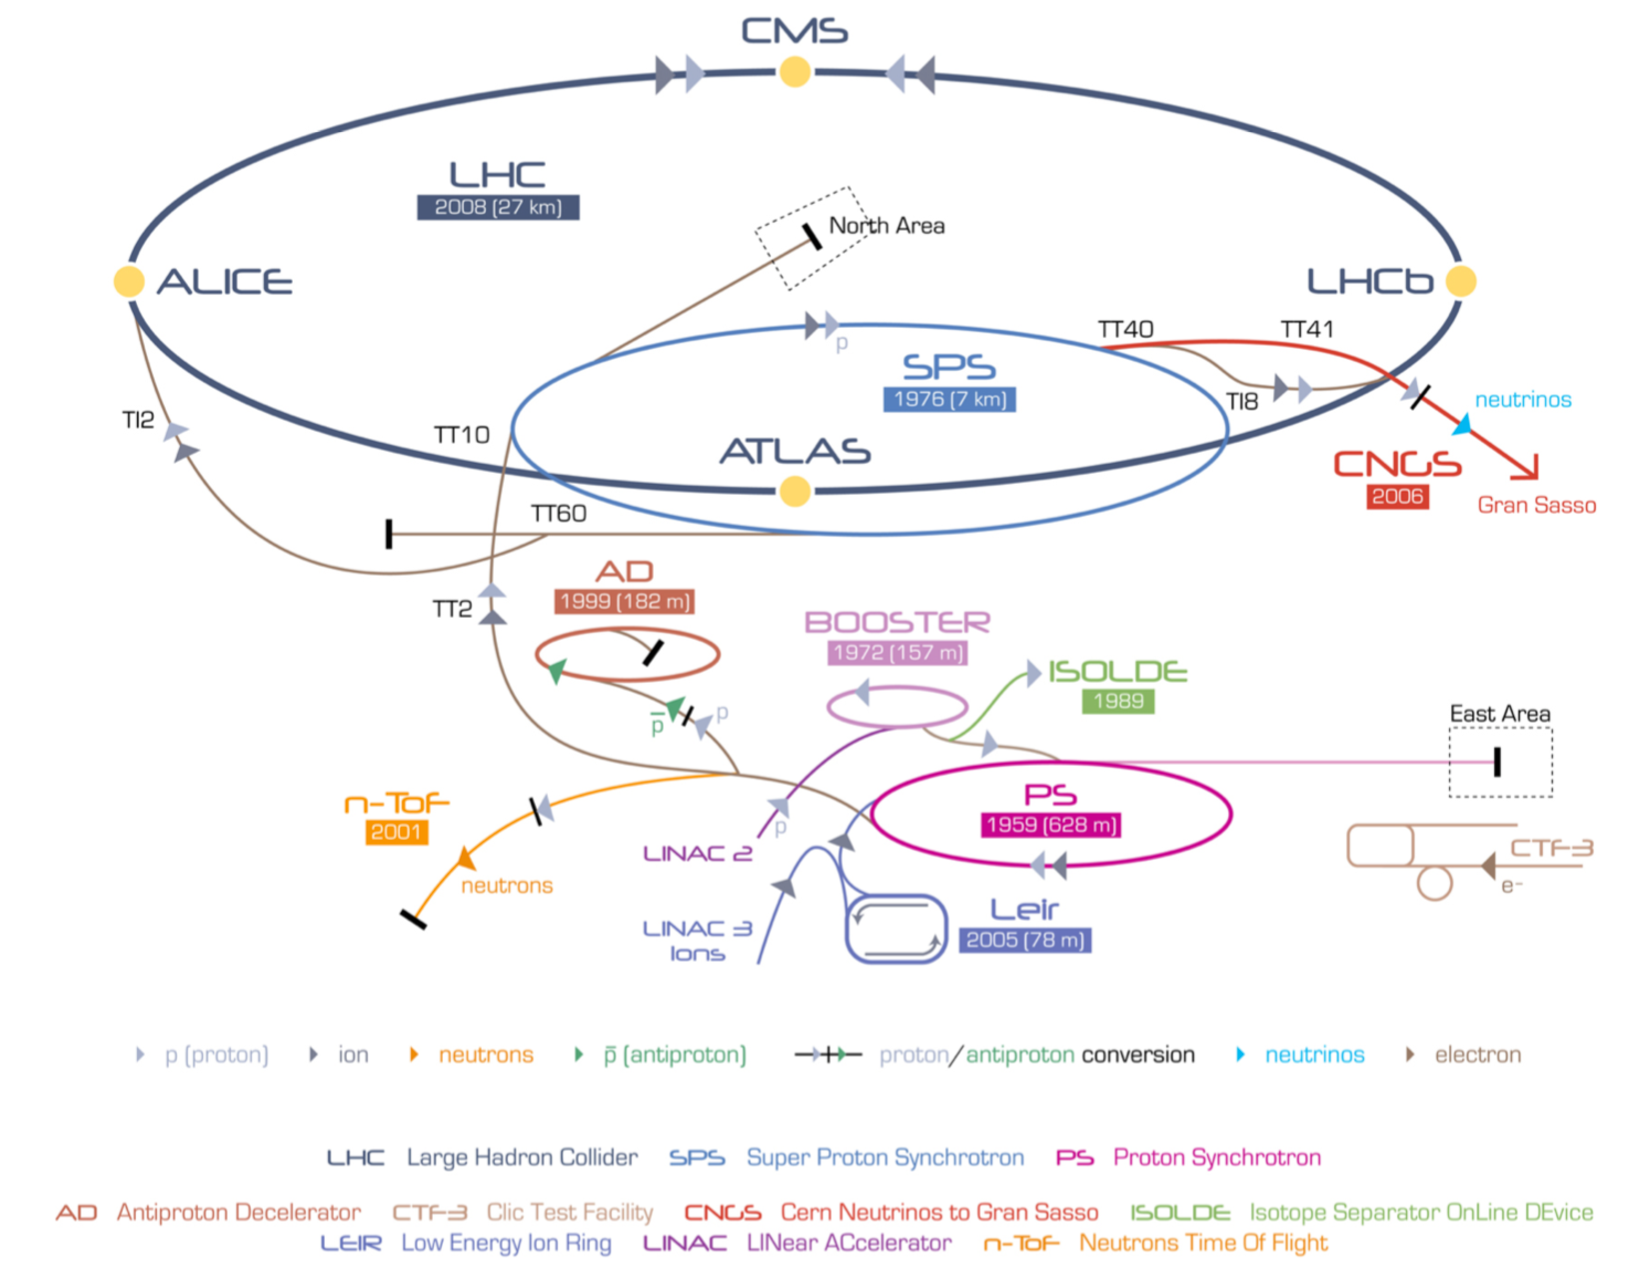
\includegraphics[width=0.75\textwidth, trim=2cm 0cm 1cm 1cm,clip]
                  {CERNaccelerators}
  \caption{The CERN experiments and accelerators}
  \label{fig::CERNaccelerators}
\end{figure}

The COMPASS spectrometer is a two-stage spectrometer.  The two stages are series
where each stage contains various tracking detectors and a muon wall filter at
the end of each stage.  Any particles that penetrate through the active area of
either of the muon wall filters are with a high probability, muons.  Both stages
also contain an electromagnetic and hadron calorimeter.  The stages are both
centered around a strong spectrometer magnet used for determining particle
momentum.  The first stage downstream of the target is the large angle
spectrometer (LAS) and it is centered around the SM1 magnet which has an
integrated field of 1~Tm.  This stage detects tracks with larger polar
scattering angles roughly between 26~mrad and 160~mrad.  The second stage is the
small angle spectrometer (SAS) and it detects particle tracks having a
scattering angle between roughly 8~mrad and 45~mrad.  This stage is centered
around the SM2 magnetic which has an integrated field of 4.4~Tm. \par

The left and right side of the spectrometer are referred to by the mountains
that surround the spectrometer.  When looking down the beam line the left side
is referred to as the Jura side which roughly corresponds to the west side and
the right side is referred to as the Saleve side which roughly corresponds to
the east side.  A graphic of the 2015 setup is shown in
Fig~\ref{fig::compassSpec}.\par

This chapter gives an overview of the general COMPASS data taking setup and
highlights the specific features in 2015.  All the data in this thesis was
produced with the 2015 setup.  For a more thorough review of the spectrometer
see reference~\cite{compassSpec}.  This chapter is roughly organized by how the
data taking occurs and concludes with an extra section summarizing the unique
features of the 2015 Drell-Yan data taking conditions. \par

\begin{figure}[h!t]
  \centering
  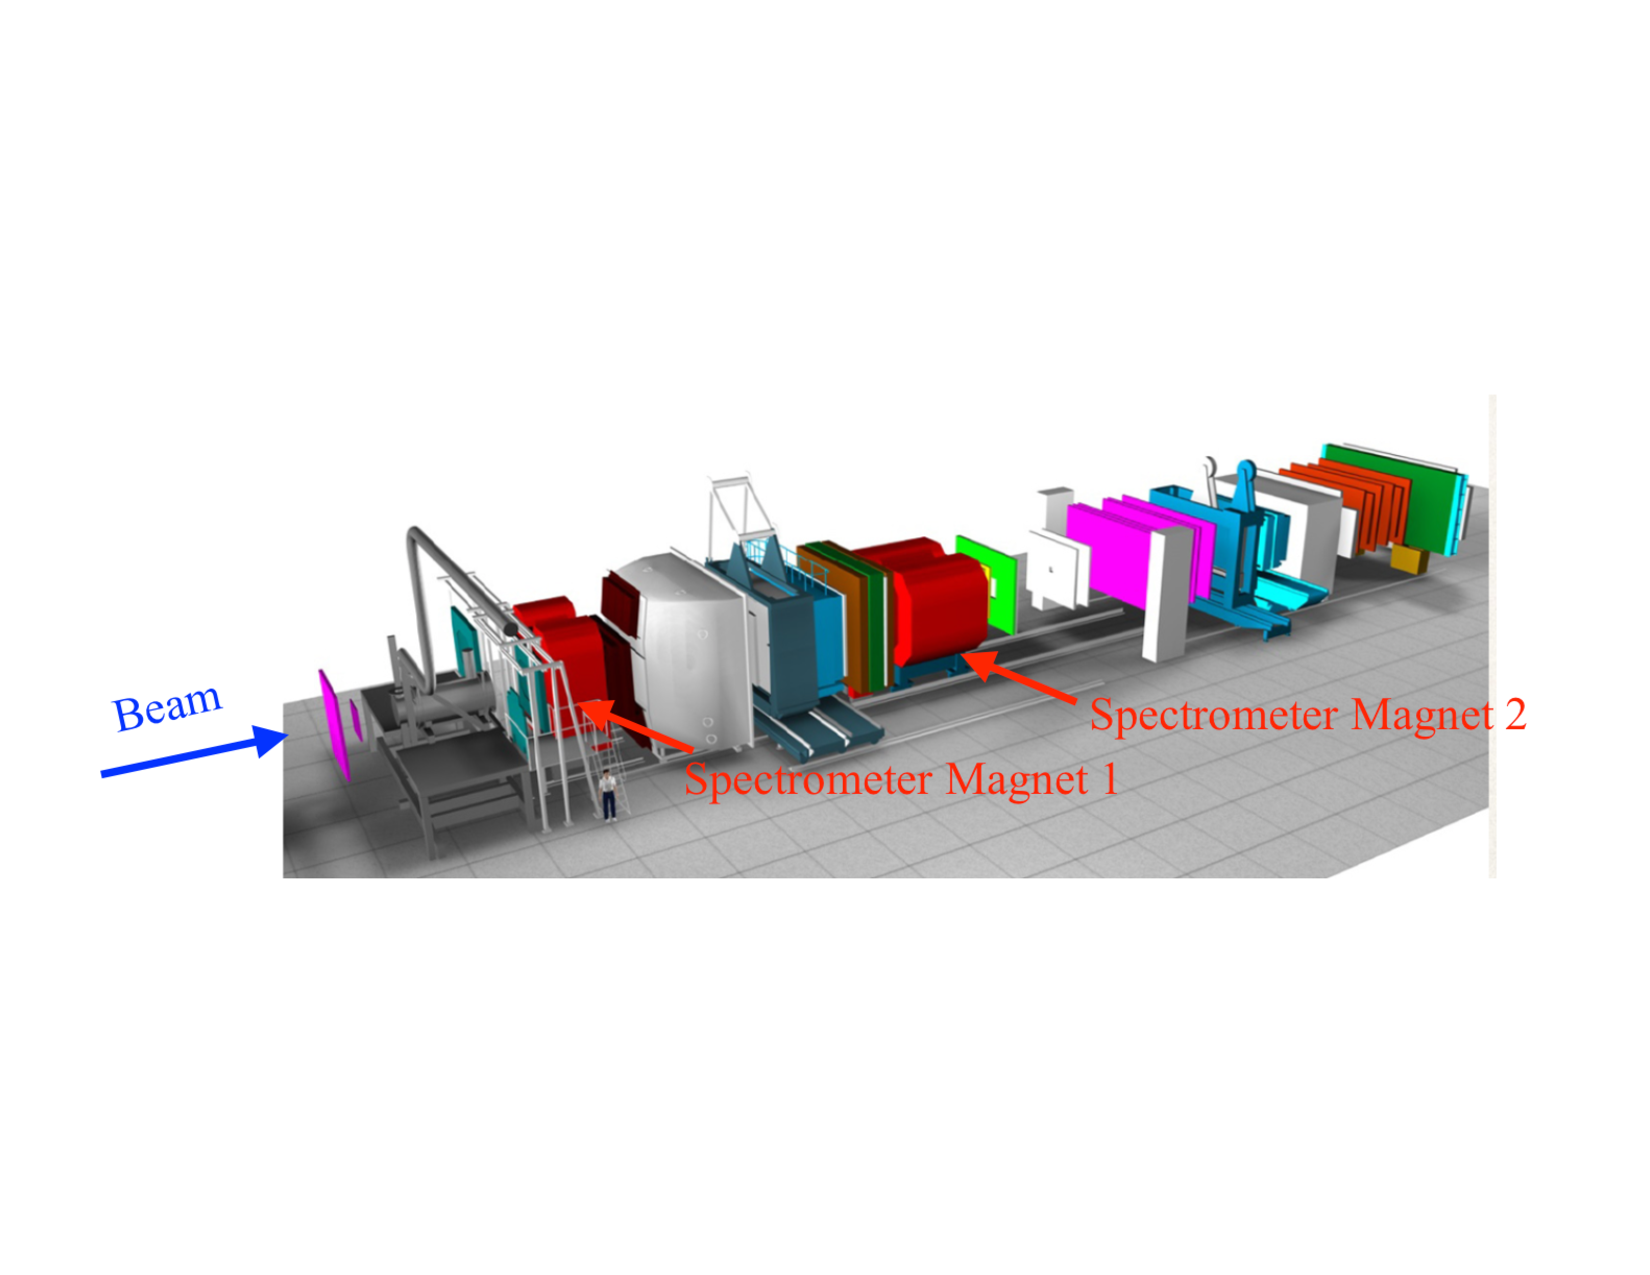
\includegraphics[width=\textwidth, trim=0.5cm 7cm 0.7cm 7cm,clip]{compassSpec}
  \caption{A schematic of the 2015 COMPASS setup}
  \label{fig::compassSpec}
\end{figure}

\section{The Beam}
The COMPASS spectrometer receives beam from the Super Proton Synchrotron along
the M2 beam line.  A schematic of the components in the M2 beam line is shown in
Fig.~\ref{fig::M2line}.  The SPS is the second largest accelerator at CERN with
a circumference of almost 7 km which accelerates protons up to an energy of
450~GeV.  The SPS extracts beam to famous Large Hadron Collier and as well sends
beam to various experiments in the North Area at CERN.  While the COMPASS
spectrometer is above ground, the SPS is below ground and the M2 beam line must
bend the beam from below ground to ground level. \par

There are several different beam types and energies available to COMPASS.  The
beam types used for physics analysis are a tertiary muon beam up to 190~{\gvc}
and secondary hadron beam with an energy up to 280~{\gvc}.  Both of the previous
beam types can have a positive or negative charge.  As well as the other two
beam types it is also possible to have a low intensity tertiary electron beam,
mainly used for calibrations. \par

\begin{figure}[h!t]
  \centering
  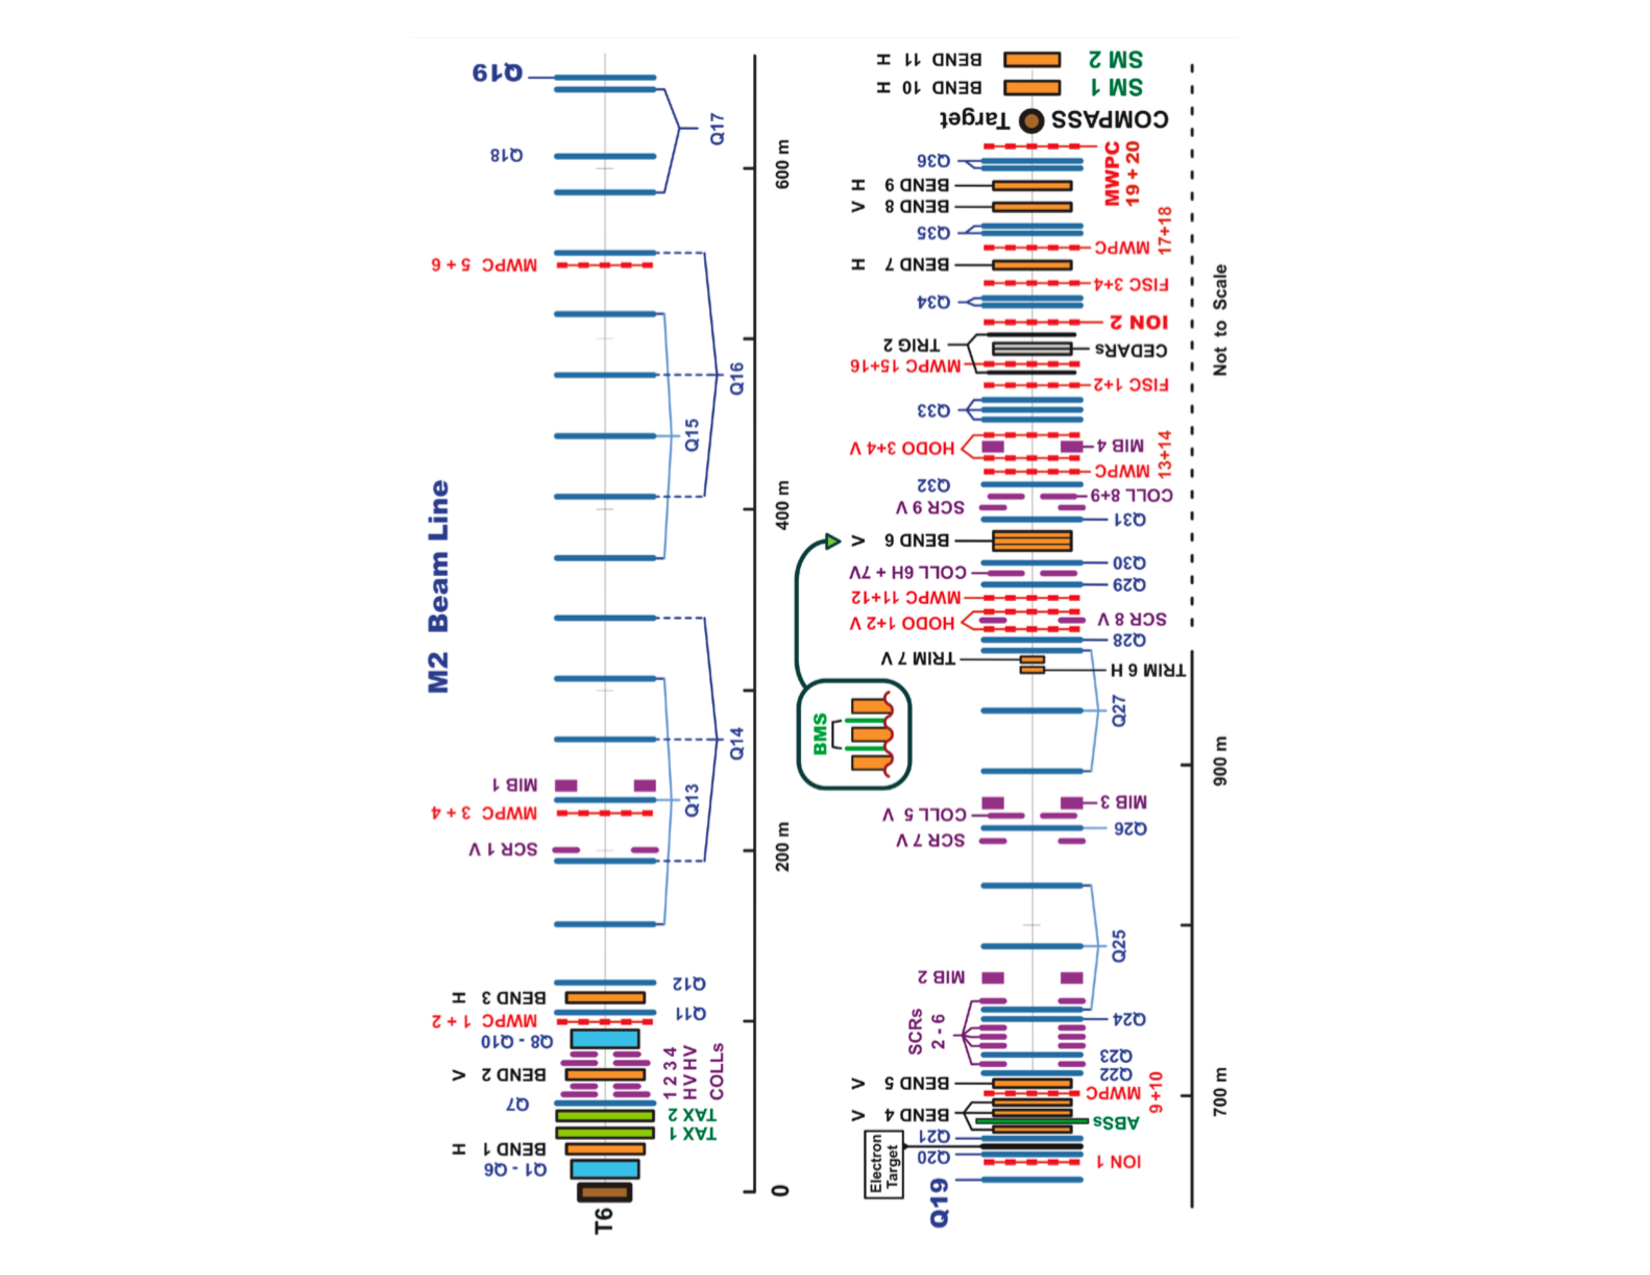
\includegraphics[width=\textwidth,trim=2cm 0cm 6cm 0cm,clip,angle=270]{M2line}
  \caption{The M2 beam line at CERN}
  \label{fig::M2line}
\end{figure}

The start of the M2 beam line is the T6 target.  The SPS can accelerates primary
protons up to 400~{\gvc} to impinge on this T6 target which produces a secondary
beam.  The nominal proton intensity on the T6 target is 100x10$^{11}$
spill$^{-1}$.  The T6 target is made of beryllium and has an adjustable length.
The longer the T6 target the higher the secondary intensity where 500mm is the
longest and typical target length used for physics data taking.  The reaction of
the proton beam with the T6 mainly produces secondary protons, pions and kaons.
Following this reaction a series of dipole and quadruple magnets select the
momentum and charge of interest. \par

The SPS spill structure varies throughout the data taking year depending mainly
on the needs of the Large Hadron Colider (LHC).  In 2015 the average intensity
provided was 0.6x10$^8$ s$^{-1}$ and the typical spill structure was two
4.8~second spills every 36~seconds.

\subsection{Muon Beam}
The muon beam is a tertiary beam which results from a weak decay of the
secondary beam.  After the initial proton reaction on T6 the resulting secondary
particles are momentum and charge selected and sent through a 600m tunnel with
focusing and de-focusing (FODO) quadruple magnets.  In this tunnel the secondary
pions and kaons can decay as
\begin{equation}
  \pi^{-(+)} \rightarrow \mu^{-(+)} + \overline{\nu}_{\mu^-}(\nu_{\mu^+})
  \label{eqn::pionDecay}
\end{equation}
\noindent
and
\begin{equation}
  \mathrm{K}^{-(+)} \rightarrow \mu^{-(+)} +
  \overline{\nu}_{\mu^-}(\nu_{\mu^+}),
  \label{eqn::kaonDecay}
\end{equation}
\noindent
where K$^{-(+)}$ is a kaon of negative or positive charge.  At the end of the
tunnel, a series of nine 1.1~m long beryllium absorbers, referred to as the ABS
in Fig.~\ref{fig::M2line}, remove the remaining hadron component which did not
decay.  A 172~{\gvc} secondary pion beam is chosen to achieve a 160~{\gvc}
tertiary muon beam.  Due to the fact that the neutrino in the reactions
\ref{eqn::pionDecay} and \ref{eqn::kaonDecay} is always left handed, the muon
will naturally be longitudinally polarized.  For the muon momentum chosen, the
muon beam achieves a polarization of 80\%.

\subsection{Hadron Beam}
To deliver a hadron beam to COMPASS the ABS absorbers are not used.  The decayed
muons used for the tertiary muon beam have a lower momentum than the hadron beam
and are therefore removable by magnetically rejecting these lower momentum
muons.  In the case of a negative hadron beam as in 2015, the composition of the
beam is approximately 97~\% $\pi^-$, 2.5\% kaons and 0.5\%
$\overline{\mathrm{p}}$. The 2015 Drell-Yan data taking was performed with a
190~{\gvc} hadron beam. \par

\subsection{Additional Beam Line Components} \label{sec::addBeam}
After the decay tunnel the beam is bent upwards along another FODO tunnel.  The
lenght of this tunnel is 250m and reaches the surface level approximately 100m
before the COMPASS target.  A series of three dipole magnets, called bend 6,
then bend the beam to a horizontal position aimed at the COMPASS target.  Both
upstream and downstream of bend 6, there are three tracking detectors
(BM01-BM06) that make up the Beam Momentum Station (BMS).  The BMS is the
upstream most component of the COMPASS spectrometer.  It is able to determine
the beam momentum to better than 1\% of the beam momentum with an efficiency of
approximately 93\%.  Bend 6 and the BMS are shown schematically in
Fig.~\ref{fig::BeamLine1}. \par

\begin{figure}[h!t]
  \centering
  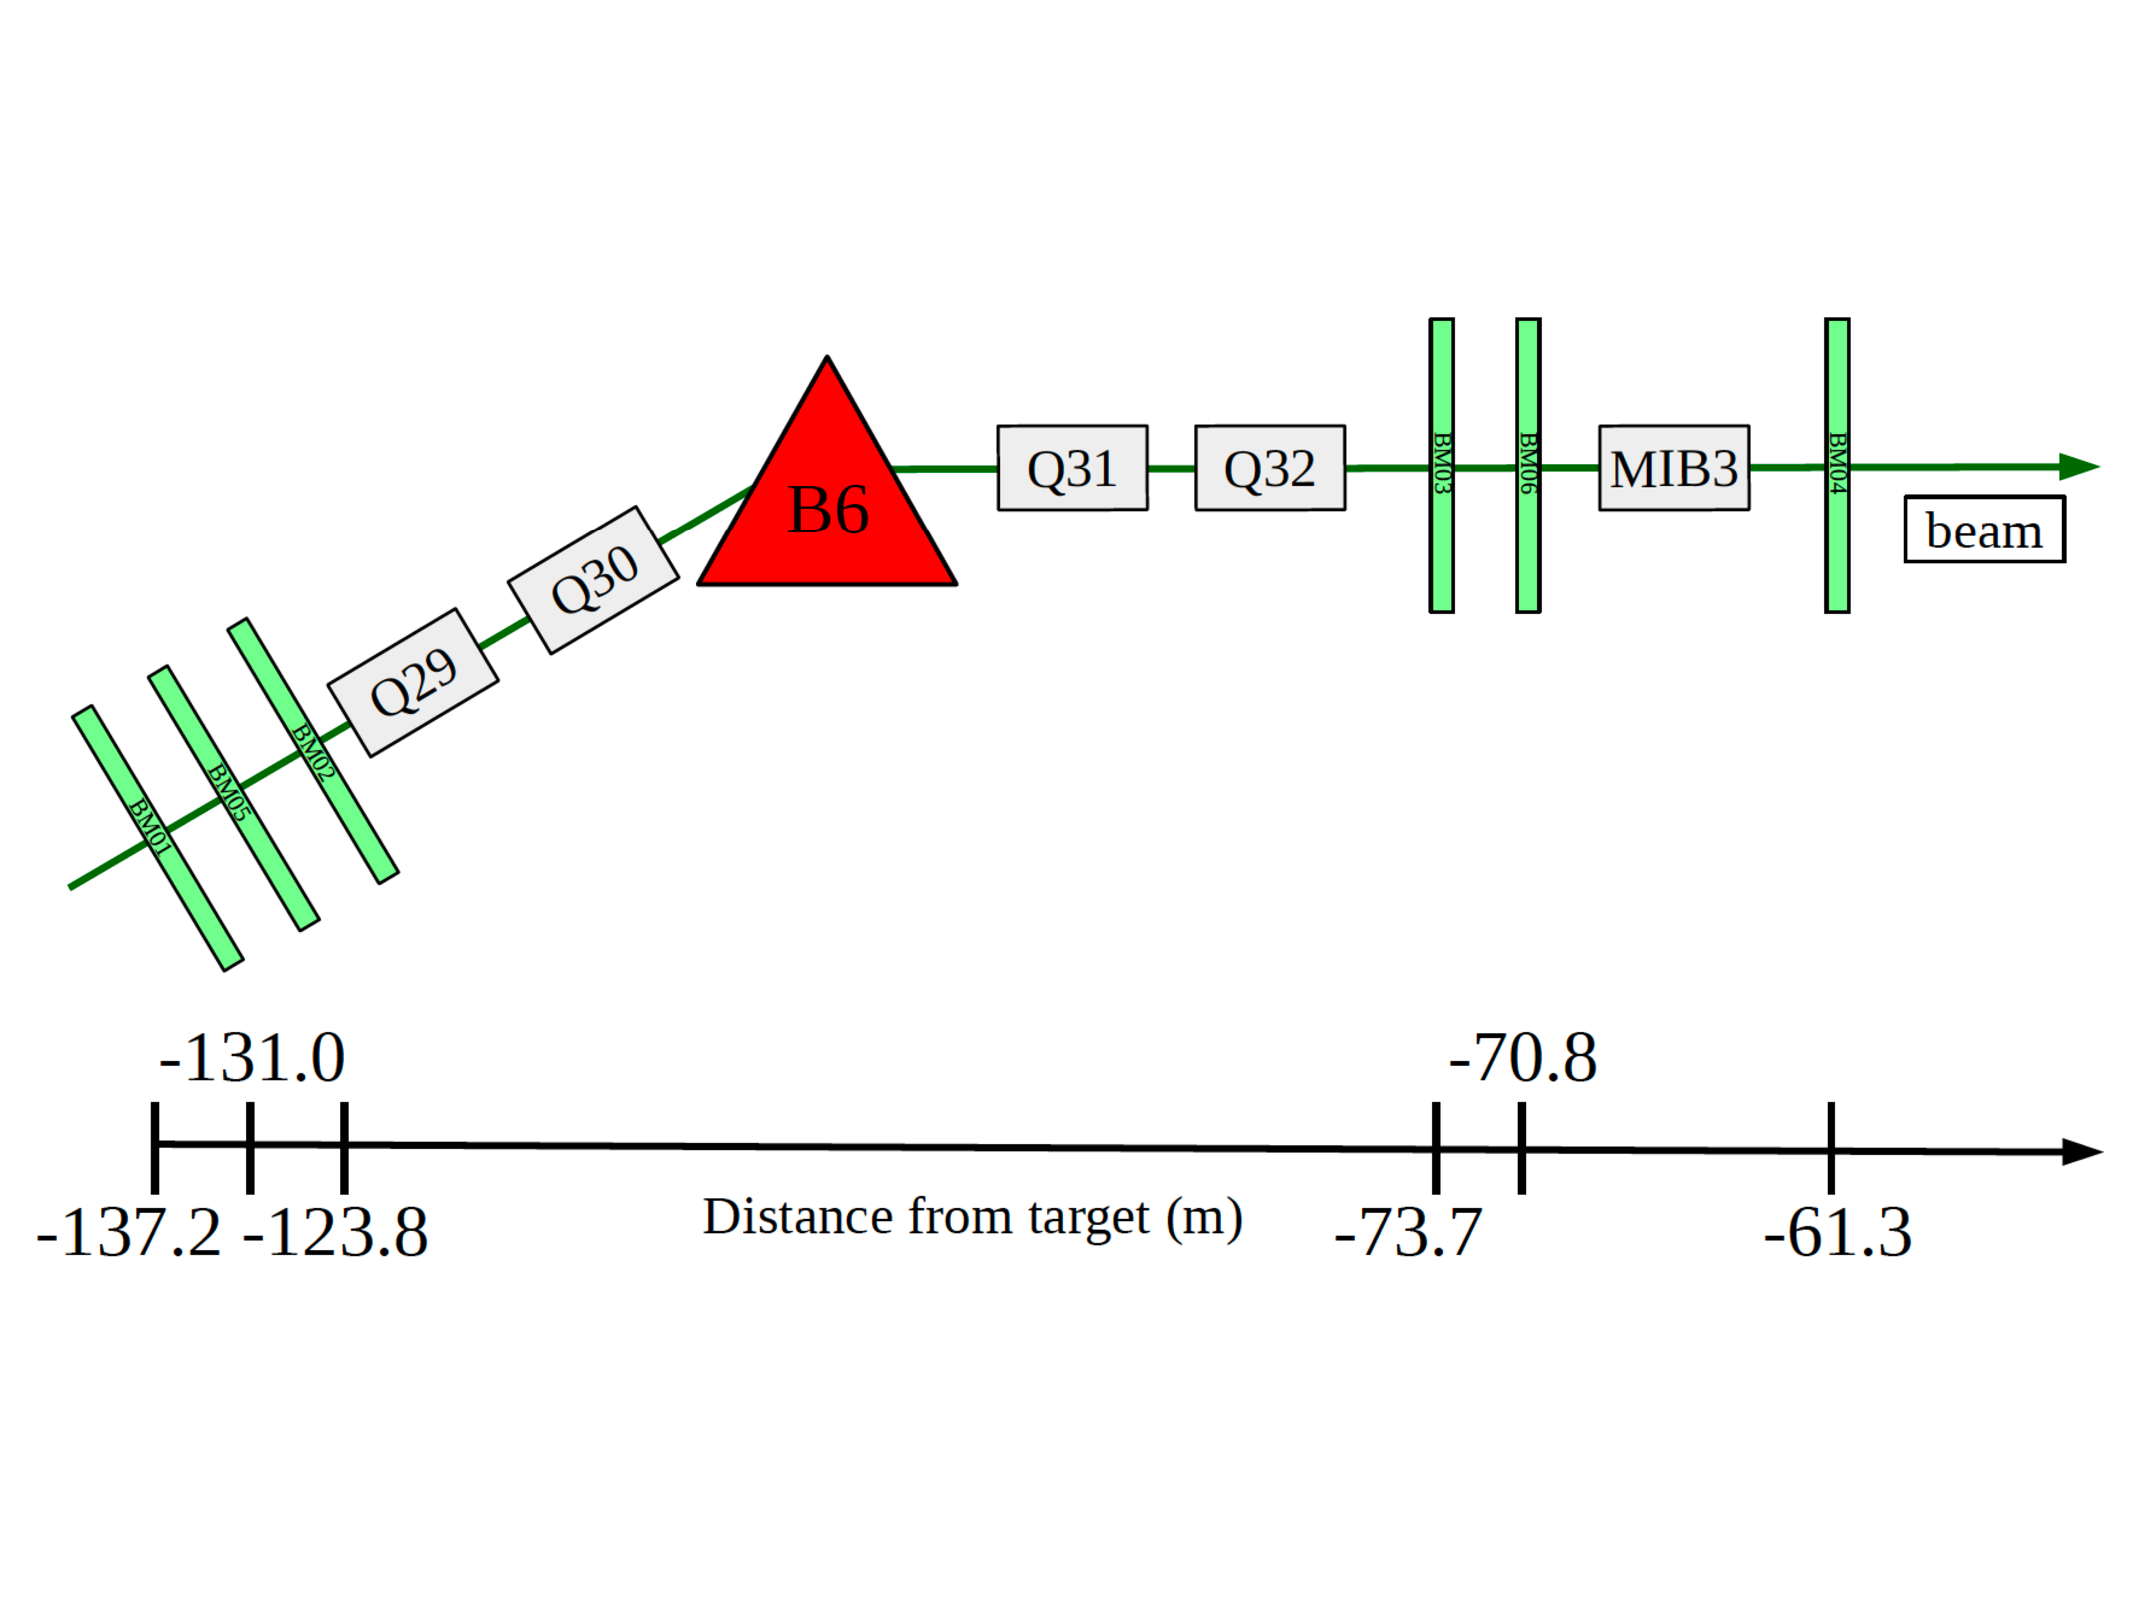
\includegraphics[width=0.8\textwidth]{BeamLine1}
  \caption{Bending the beam to a horizontal position.  The BMS detectors are
    upstream and downstream of the bend 6 magnet.}
  \label{fig::BeamLine1}
\end{figure}

During the 2015 Drell-Yan setup the $\pi^-$ beam intensity was too high for the
BMS station to work properly.  For this reason, special low intensity,
approximately 10$^6$ s$^{-1}$, $\pi^-$ beams were used in 2014 to determine the
momentum distribution during Drell-Yan data taking.  The beam momentum
distribution is shown in Fig.~\ref{fig::BeamMomBMS} where the average momentum
is 190.9~{\gvc} with a spread of $\pm$ 3.2~{\gvc}. \par

\begin{figure}[h!t]
  \centering
  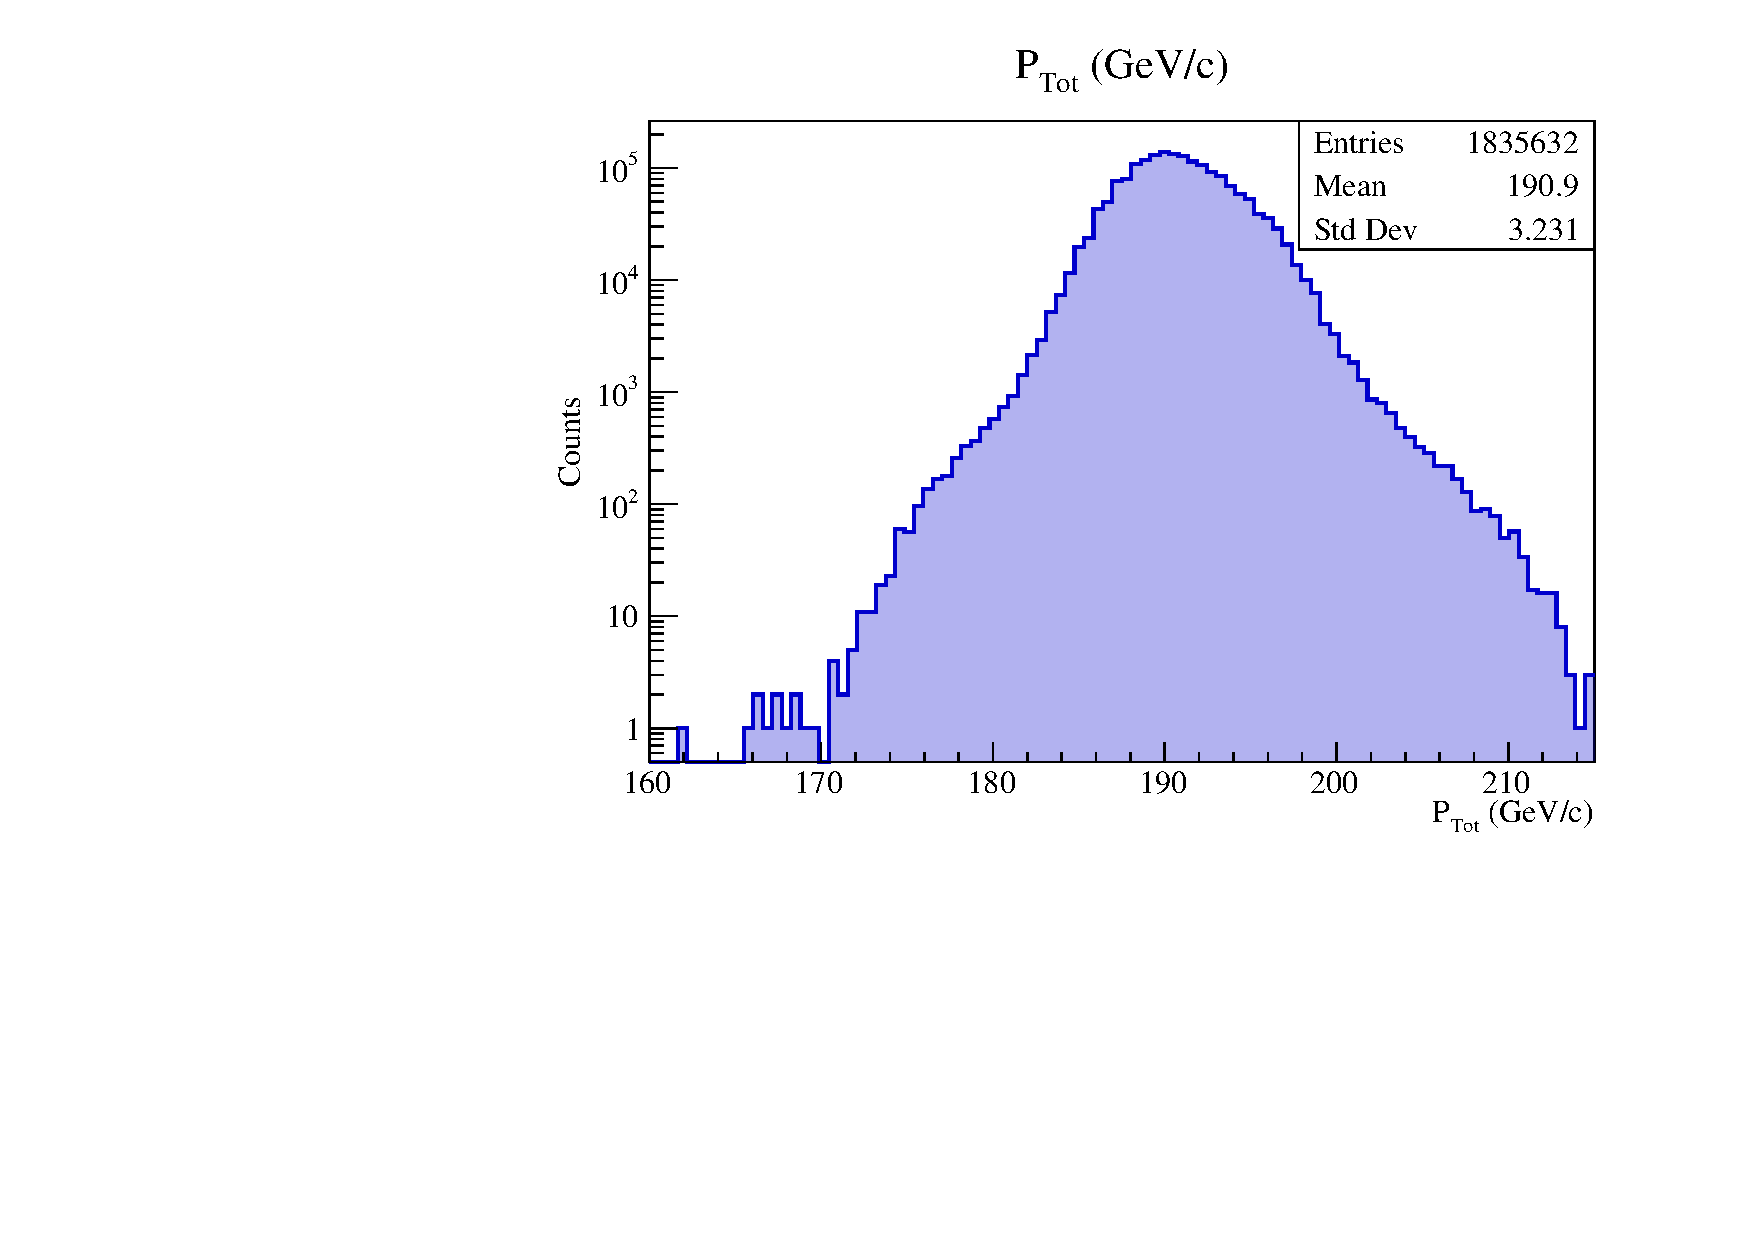
\includegraphics[width=0.5\textwidth]{BeamMomBMS}
  \caption{The momentum distribution of the $\pi^-$ beam, determined during
    dedicated low intensity beam conditions}
  \label{fig::BeamMomBMS}
\end{figure}

Approximately 30~m upstream of the target are to two Cherenkov counter (CEDAR)
detectors.  As the hadron beam has contamination from several components these
CEDARs can be used to distinguish between the different components.  The CEDARs
at COMPASS are high pressure detectors and have been demonstrated to achieve
fast particle identification for particle momentums up to 300~{\gvc}.  The
CEDARs general principle of operation is that two particles with the same
momentum but different mass will emit Cherenkov radiation at different angles
relative to their momentum.  When a particle is traveling faster than the speed
of light in a given medium, it emits Cherenkov radiation in a cone centered
along its momentum axis.  The faster the particle is traveling the narrower the
angle of the Cherenkov light cone.  A schematic of the CEDAR operating principle
is shown in Fig.~\ref{fig::cedars}.  In 2015 the CEDARs were measured to be
largely inefficient due to the high beam intensity and are not used for the
analysis of this thesis.

\begin{figure}[h!t]
  \centering
  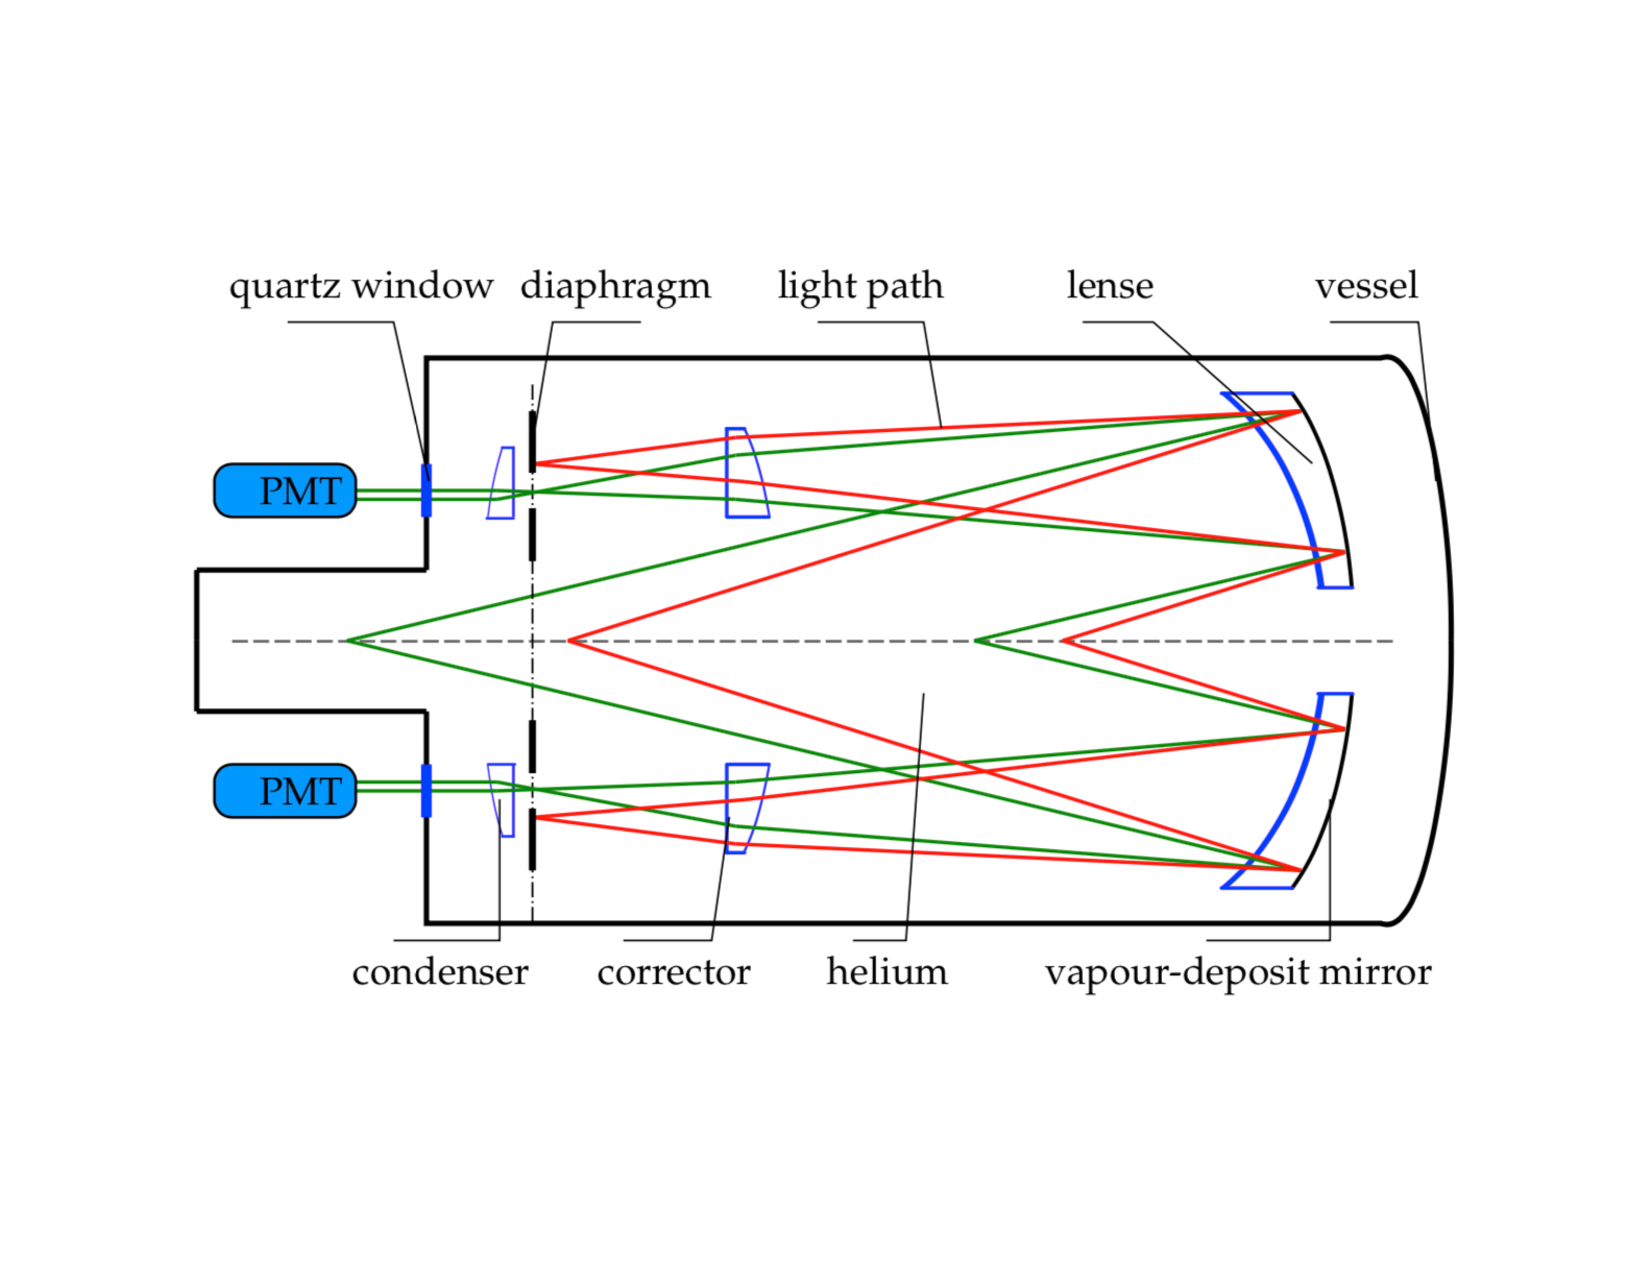
\includegraphics[width=0.5\textwidth,trim=2cm 4cm 2cm 4cm,clip]{cedars}
  \caption{Light lines emitted inside CEDARs at COMPASS.  The
    red(green) lines correspond to Cherenkov light emitted from a particle.}
  \label{fig::cedars}
\end{figure}

For years with a transversely polarized target, such as 2015, a chicane system
of dipole magnets is setup in front of the target.  The chicane first bends the
beam away from the beam line and then back to the target such that the beam hits
the target at an angle.  A chicane magnet setup is used because a beam hitting
the target without any angle would then be deflected from the target magnet to
the left or right of the spectrometer.  For this reason the chicane gives the
beam an angle before hitting the target such that the non-interacting beam exits
the target traveling straight towards the spectrometer.


\section{The Polarized Target}
The polarized target at COMPASS is the most complicated and essential component
of the spectrometer.  It is located upstream of the tracking detectors and
spectrometer magnets and downstream of the beam telescope, described in
section~\ref{sec::tracking}, detectors.  The target consists of two or three
cylindrical cells.  The possible materials are either solid state ammonia
(NH$_3$) or deuterated lithium ($^6$LiD) or liquid hydrogen. Fig.~\ref{fig::PT}
shows a schematic of the target.  \par

\begin{figure}[h!t]
  \centering
  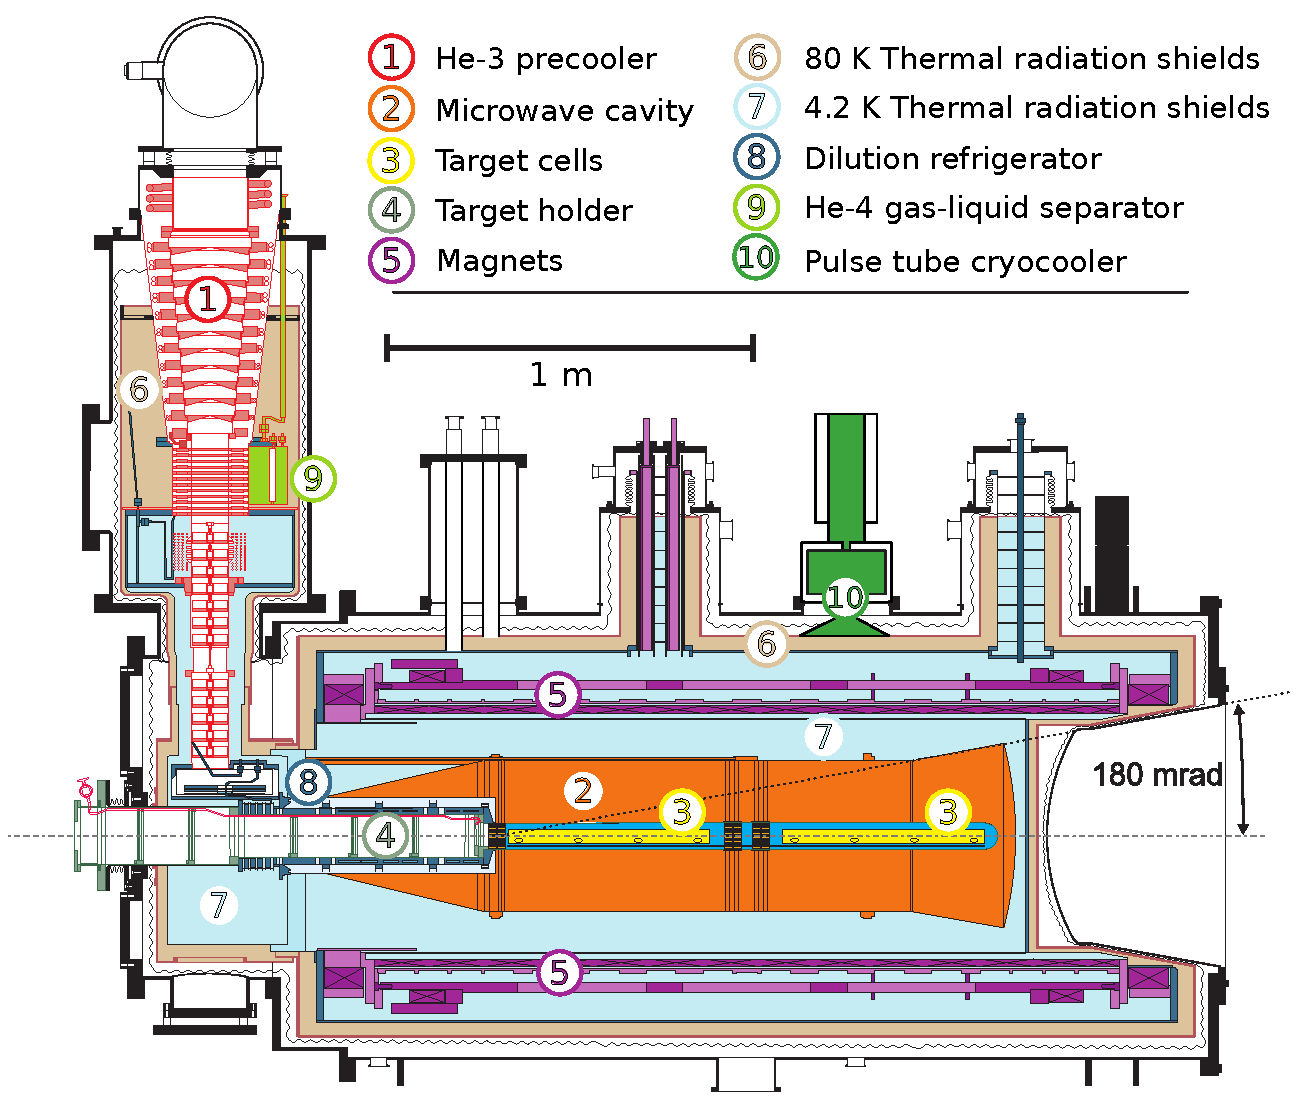
\includegraphics[width=0.8\textwidth]{PT}
  \caption{The polarized target at COMPASS}
  \label{fig::PT}
\end{figure}

Surrounding the cylindrical cells is a longitudinal super conducting magnet
capable of reaching a magnetic field of 2.5~T.  This longitudinal magnet
polarizes the target parallel or anti-parallel to the direction of the beam
momentum.  The target polarization is maintained by keeping the target in a
liquid helium bath of approximately 60~mK.  This is called frozen spin mode
where the temperature is maintained by a dilution refrigerator. \par

The target is polarized through the dynamic nuclear polarization (DNP)
method~\cite{DNPmethod}.  This process works by first polarizing electrons in
the target with the longitudinal magnet.  With a high probability, the target
electrons are all polarized in the same longitudinal direction for each target
cells.  Due to their much lower mass, electrons have a larger magnetic moment
and therefore can be polarized at a much faster rate than protons or neutrons.
At the same time the electrons are being longitudinally polarized, microwave
electromagnetic radiation is sent through each target cell.  For atoms which
have a nuclear spin it is then possible for these atoms to absorb a microwave
going to an excited state with the electron spin anti-parallel to the magnet and
the nuclear spin either parallel or anti-parallel to the magnet depending on the
microwave frequency.  To ensure only one frequency enters each target cell,
there is a microwave stopped between each target cell.  The electron with the
anti-aligned spin will then quickly have its spin realigned while the nucleon
will take much longer to lose its polarization due to its smaller magnetic
moment.  This process can continue in this way resulting in a net nuclear
polarization.  Using the DNP method the target can achieve a polarization of
approximately 90\% in three days. \par

The target also includes a 0.63T transverse dipole magnet to change from
longitudinal polarization to transversely polarized.  The target must first be
longitudinally polarized before the transverse target magnet can change the
polarization direction.  Once the target is transversely polarized, the target
polarization can no longer be increased as microwaves can no longer shine on the
target in the polarization direction.  Therefore the polarization will decrease
exponentially.  In 2015 the target was polarized for about half a day between
data taking sub-periods ad achieved an average polarization of 0.73\%, including
the effects of exponential polarization lose with time.  The target transverse
polarization relaxation time was about 1000 hours in 2015. \par

The target polarization was measured with 10 NMR coils while the target cells
were longitudinal polarized.  In the 2015, each target cell had the most
upstream and downstream coils in the center of the target cell and the other
three coils on the outside perimeter as is shown in Fig.~\ref{fig::targCells}.
Due to the fact that the polarization can only be measured with the longitudinal
magnet on, the polarization is only measure at the start and finish of a
transversely polarized data taking.  The intermediate polarization is then
determined by exponential interpolating between these two times.

\begin{figure}[h!t]
  \centering
  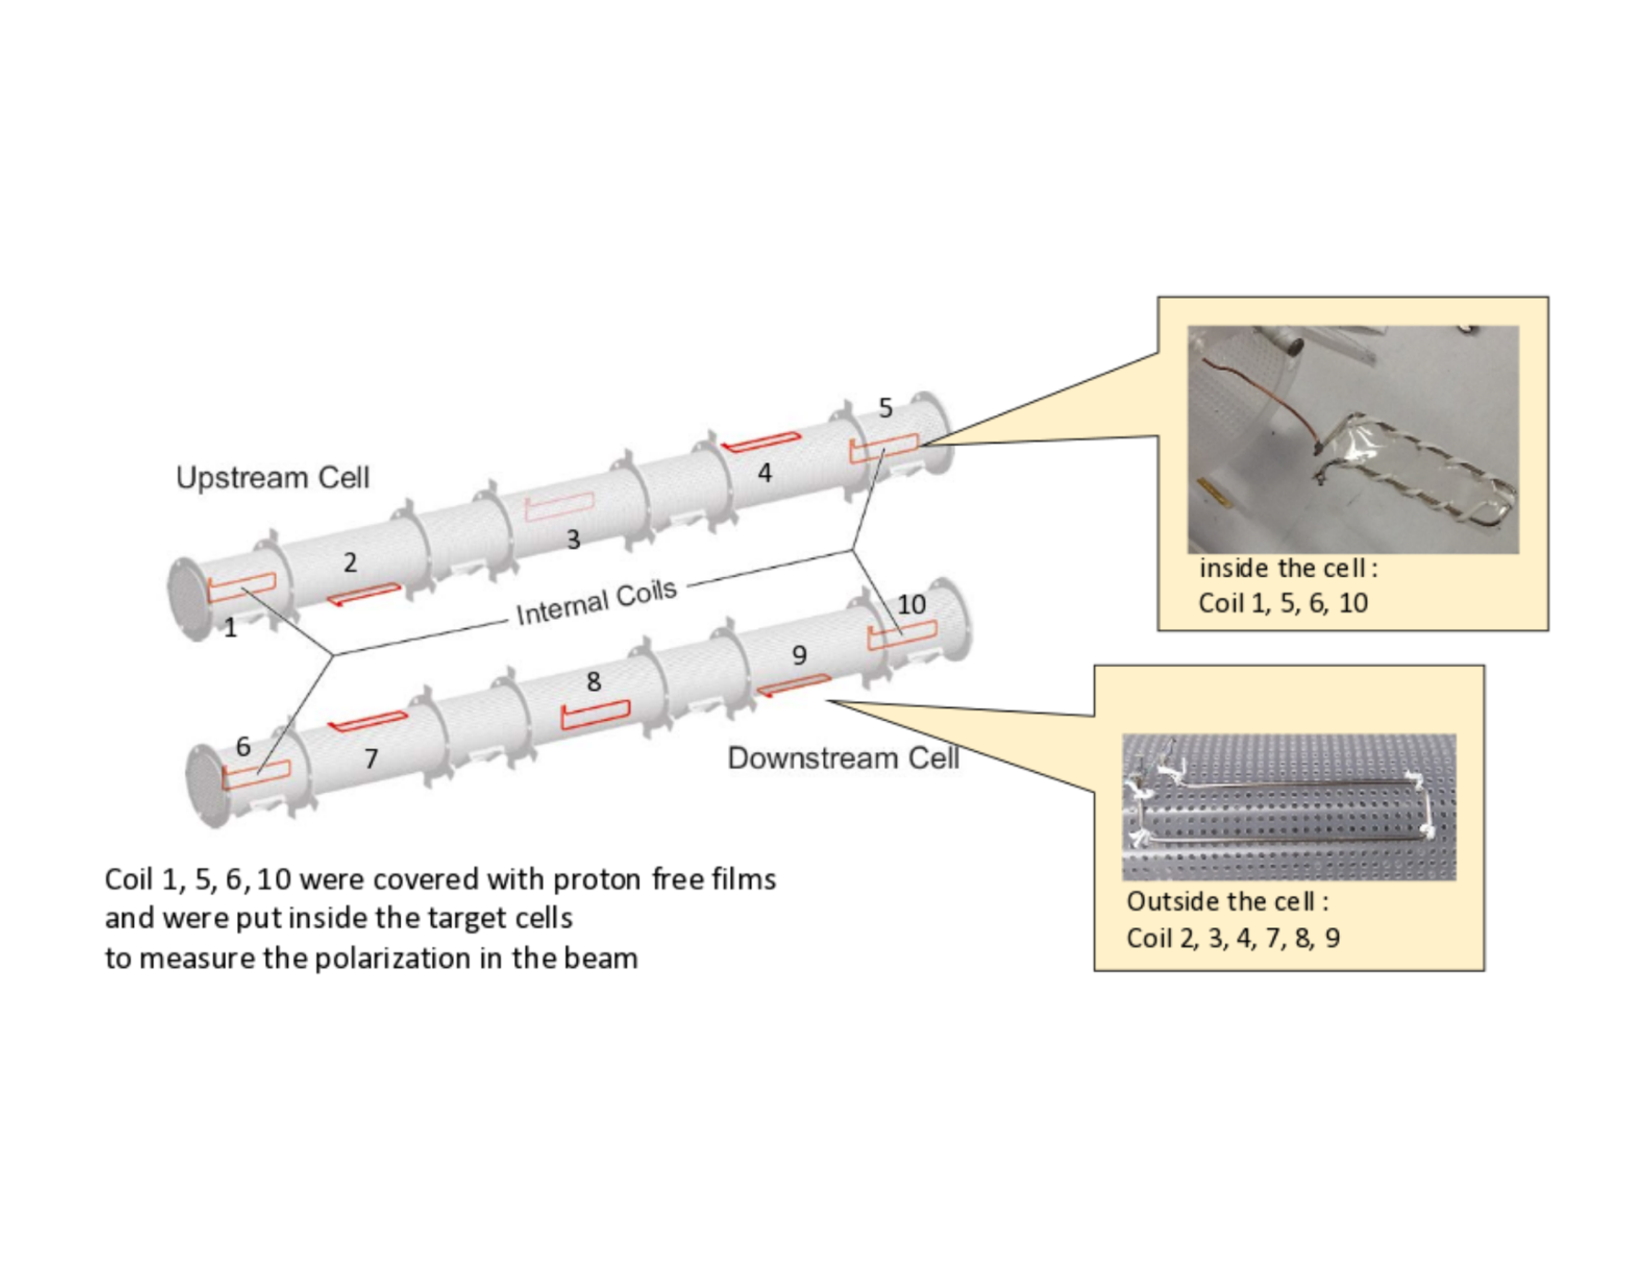
\includegraphics[width=0.8\textwidth]{targCells}
  \caption{The empty polarized target cells side by side along with their NMR
    coil positions}
  \label{fig::targCells}
\end{figure}

In 2015 the setup was two transversely polarized target cells of 55~cm length
and 2~cm in radius.  The cells were separated by 20~cm and polarized in opposite
directions.  The polarization of the target cells was flipped ever two weeks of
data taking to reduce systematic effects from luminosity and geometrical
spectrometer acceptance.  Due to the fact that the beam needs to be precisely
steered onto the target and that the chicane magnets upstream of the target are
setup for only one transverse target magnet direction, the transverse target
magnet only pointed downward in 2015.  To achieve a polarization flip the target
polarization had to therefore be rotated back to the longitudinal direction and
the input microwaves had to be changed to achieve the desired polarization
direction. \par

The target material in 2015 was solid state NH$_3$.  The protons in the three
hydrogen atoms were the only nucleons with nuclear spin and therefore only some
fraction of the target was able to be polarized.  The fraction of polarized
nucleons to total nucleons is called the dilution factor.  Counting the ratio of
unpolarized nitrogen nucleons to polarized hydrogen, one would expect the
dilution to be 3/17.  However to get a more accurate determination of the
dilution factor the follow calculation was used

\begin{equation}
  f = \frac{n_H\sigma^{DY}_{\pi^-H}}
  {n_h\sigma^{DY}_{\pi^-H} + \sum_A n_A\sigma^{DY}_{\pi^-A}},
\end{equation}
where $f$ is the dilution factor, $n_H$ is the number of hydrogen atoms in
NH$_3$, $n_A$ is the number of other nucleons in NH$_3$, and
$\sigma^{DY}_{\pi^-H}$ and $\sigma^{DY}_{\pi^-A}$ are the Drell-Yan
cross-section for pion hydrogen scattering and pion nucleon scattering
respectively.  The cross-sections were determined using a parton-level
Monte-Carlo program MCFM~\cite{MCFM}.  The dilution factor was also further
scaled down by studies of reconstruction migration between target cells.  The
average dilution factor in 2015 was determined to 0.18 in the invariant mass
range of 4.3{\gvcs} to 8.5{\gvcs}.


\section{Tracking Detectors} \label{sec::tracking}
To determine when and where a reaction occurs in the polarized target, tracking
detectors are able to position the products the reaction.  The goal of the
tracking detectors is to determine a point in space where a particle traversed.
The COMPASS tracking detectors attempt to do this for a wide range of angles,
momentums and at different rates.  For these reasons there are several planar
tracking technologies used at COMPASS which can be divided into three
categories: very small angle tracker, small angle trackers and large area
trackers.  As the name suggest very small angle trackers measure tracks with
small angle deflections from the beam axis which are essentially beam particles.
The small area trackers measure particle tracks with low but non-zero scattering
polar angle and have small central dead zones.  The large area trackers are
several meters in height and width and measures the largest deflection angles up
to 180~mrad. \par

All of these trackers are split into stations.  Each station corresponds to
several detectors planes at roughly the same z-position along the beam line.
Each station measures a track position in one or more orientation while most
measure tracks in three or more orientations.  The coordinate orientations
measured are the X and Y coordinates which are the horizontal and vertical
directions respectfully, and as well the U and V coordinates which are rotated
at different angles with respect the X and Y coordinates. \par

\subsection{Very Small Angle Trackers}
The very small angle trackers extend up to 3~cm away from the beam axis.  This
is the region with the highest number of tracking particles and therefore these
detectors must be able to handle the highest rates up to 5x10$^7$~Hz.  The two
detector types that make up the very small angle trackers are either
scintillating fiber detectors (SciFi) or silicon microstrip detectors.  These
two detector types are complementary to each other as the former have very good
timing resolution while the latter have very good spacial resolution. \par

There are three silicon stations possible at COMPASS.  These stations have
active detecting areas of 5x7~cm$^2$.  The spacial resolution of these detectors
is nominally 10~$\mu$m and the timing resolution is nominally 2.5~ns.  For the
2015 setup, the beam intensity was too high for the silicon detectors to operate
and therefore these detectors were not used. \par

There are 10 SciFi stations available at COMPASS.  The active areas vary from
3.9x3.9~cm$^2$ to 12.3x12.3~cm$^2$ planar areas.  As well the detection fiber
diameters vary between detectors with the different diameters used at COMPASS
being 0.5~nm, 0.75~nm and 1~nm.  Several fibers are bundled together to
determine a strip hit position and the resulting nominal spacial resolutions are
130~$\mu$m, 170~$\mu$m and 210~$\mu$m.  The nominal timing resolution of these
detectors is about 400~ps.  In 2015 three SciFi stations made up the beam
telescope and were placed upstream of the target to measure the beam trajectory
and timing information.  A fourth SciFi station was place in the LAS section of
the spectrometer. \par

\subsection{Small Angle Trackers} \label{sec::SAT}
The small angle trackers detect particles with non-zero defection angles. These
detectors have medium size active areas compared to the very small angle
trackers and the large angle trackers.  They cover 5~cm to 40~cm from the beam
axis where the rate drops to approximate 10$^5$~Hz, two orders of magnitude
lower than the rates the very small angle trackers receive.  At COMPASS there
are two types of small area tracking detectors: micromesh gaseous structure
(micromegas) and gas electron multipliers (GEMs). \par

There are three micromega stations at COMPASS.  All three stations are location
sequentially after each other between the target and the first spectrometer
magnet.  As well all three detectors measure four coordinate projections and
have an active area of 40x40~cm$^2$ with a 5~cm diameter dead zone.  The
micromegas operate by having a conversion region and a smaller amplification
region.  An ionized particle produced in the conversion region will drift
through an electric field of around 3.2~kV/cm to the amplification region where
the electric field is around 50~kV/cm.  The electric field is too small for
amplification in the conversion region but as the name suggest the electric
field is high enough to amplify the signal in the amplification region.  The
amplified signal is then read out on strips.  The conversion and amplification
regions are separated by a metallic micromesh material.  The electrons pass
through the micromesh without resistance and are not rimmed out.  The micromegas
have good spacial resolution because the thickness of the amplification region
is only 100~$\mu$m, small enough to prevent much transverse spreading of the
electron avalanche between strips.  The separation of the larger conversion
region from the smaller amplification region with the micromesh prevents
electric field lines from being distorted in the conversion region and therefore
prevents the primary electrons from drifting slower in the conversion region.
This allows micromegas to operate at a higher rate than would be possible
otherwise.  This principle of operation is illustrated in
Fig.~\ref{fig::MicroMega}.  The strips in the central part of the detector are
360~$\mu$m corresponding to a resolution of about 100~$\mu$m and the strips in
the outer region are 460~$\mu$m corresponding to a resolution of about
120~$\mu$m.  The nominal timing resolution 9~ns.  In 2015 the micromegas were
upgraded to include a pixelized section covering much of the dead zone
area. \par

\begin{figure}[h!t]
  \centering
  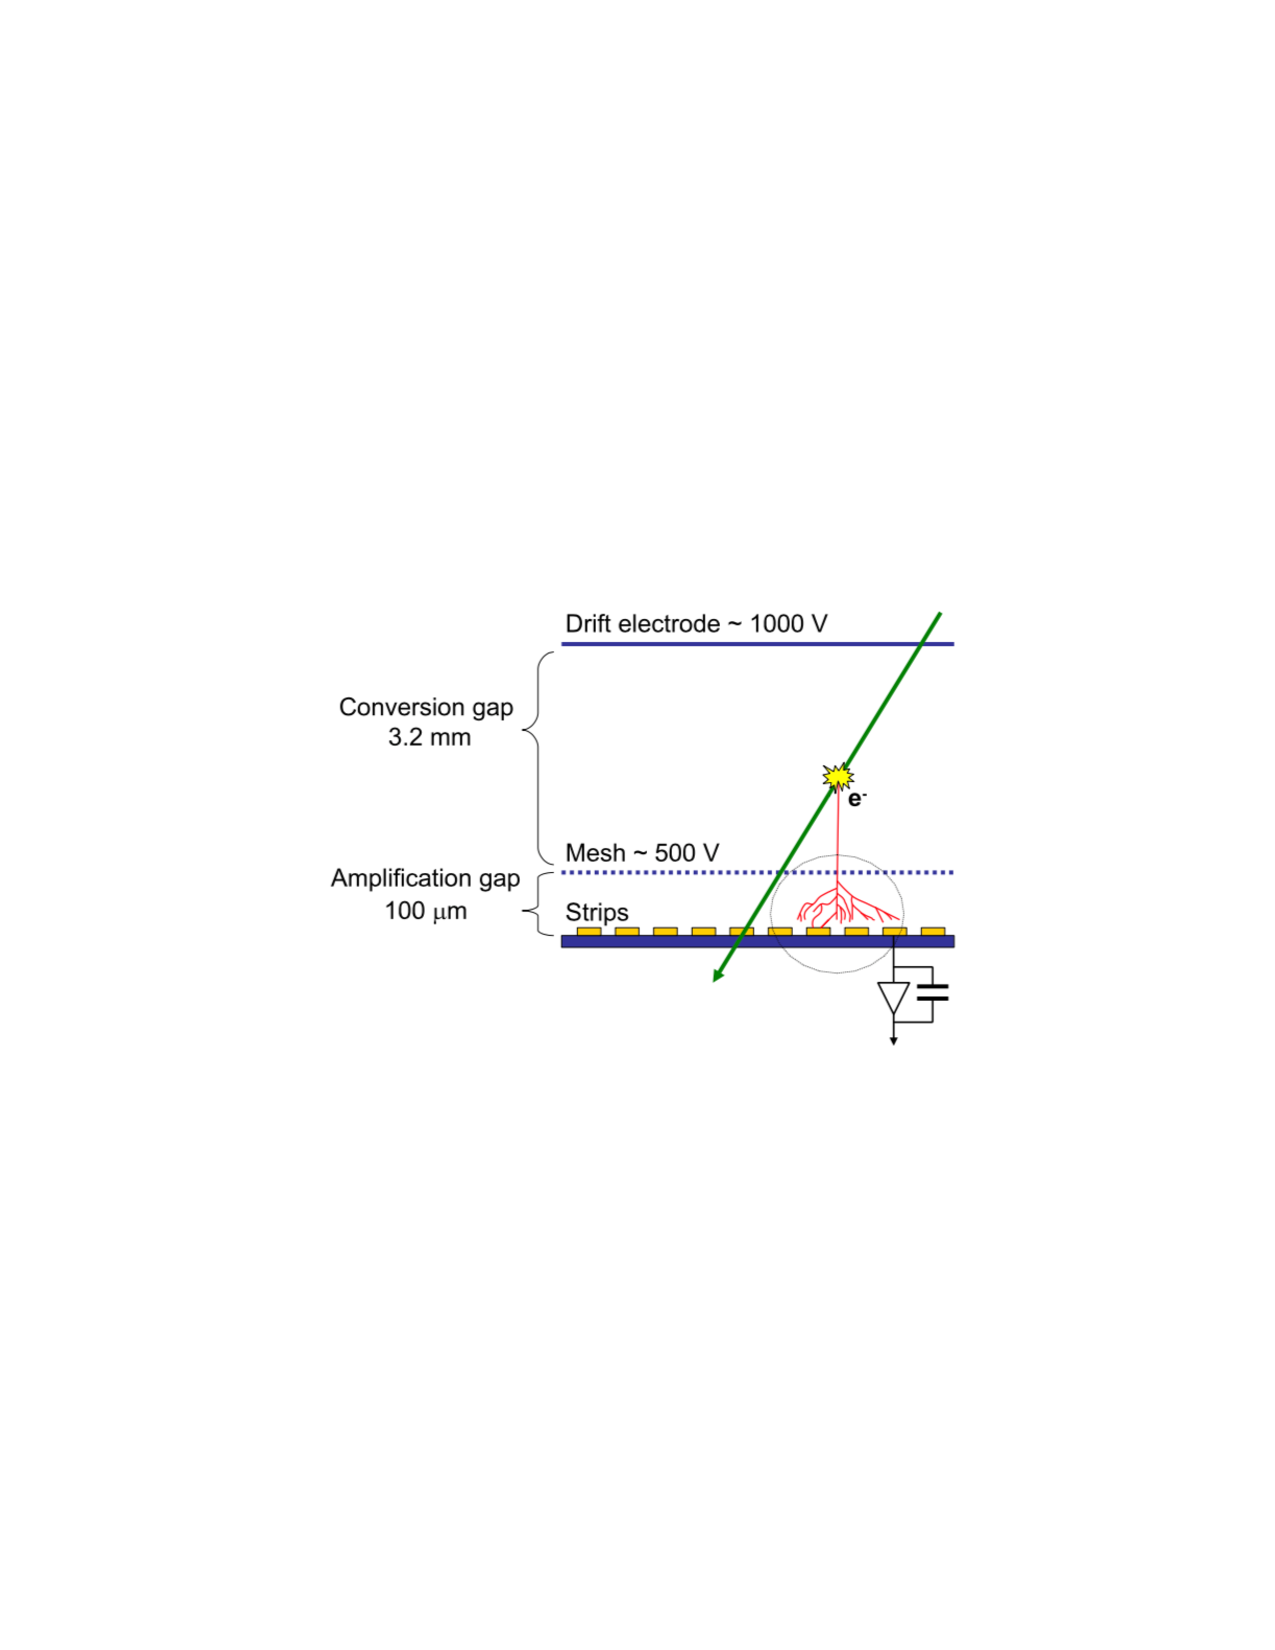
\includegraphics[width=0.7\textwidth, trim=4cm 10cm 4cm 10cm, clip]{MicroMega}
  \caption{Principle of operation for the micromesh gaseous structures
    (micromegas)}
  \label{fig::MicroMega}
\end{figure}

There are eleven GEM detectors located throughout the COMPASS spectrometer.  The
first GEMs are located after the first spectrometer magnet and the last GEMs are
located near the end of the spectrometer.  These detectors are positioned close
to the beam axis.  They are mounted on a large area tracker, covering the dead
zone region of the large area tracker.  All eleven detectors have an active area
of 31x31~cm$^2$ and a 5~cm diameter dead zone.  In times of lower beam intensity
the dead zones can be turned on as an active area.  \par

The detector is split into four regions.  These regions are separated by a
polymide foil (50~$\mu$m thick) having around 10$^4$~cm$^{-1}$ drifting holes of
70~$\mu$m diameter and are clad with copper on both sides.  There in an electric
potential of a few hundred volts between each foil layer.  The electron
amplification occurs around the holes of each of the three foil dividers.  This
means GEM detectors speed up the amplification process by splitting the
amplification avalanche into three locations.  The process is sped up because
the drifting electrons are accelerated multiple times there by speeding up their
drifting velocity which therefore reduces the overall drift time from the
ionization location to the strip readout.  This allows the GEMs to operate at a
higher rate then would otherwise be possible.  The principle of operation is
illustrated in Fig.~\ref{fig::GEM}.  The nominal timing and spacial resolution
of the GEM detectors is 10~ns and 110~$\mu$m respectively.  Two pixelized GEM
detectors where also in operation but were not as crucial for the 2015 Drell-Yan
measurement.

\begin{figure}[h!t]
  \centering
  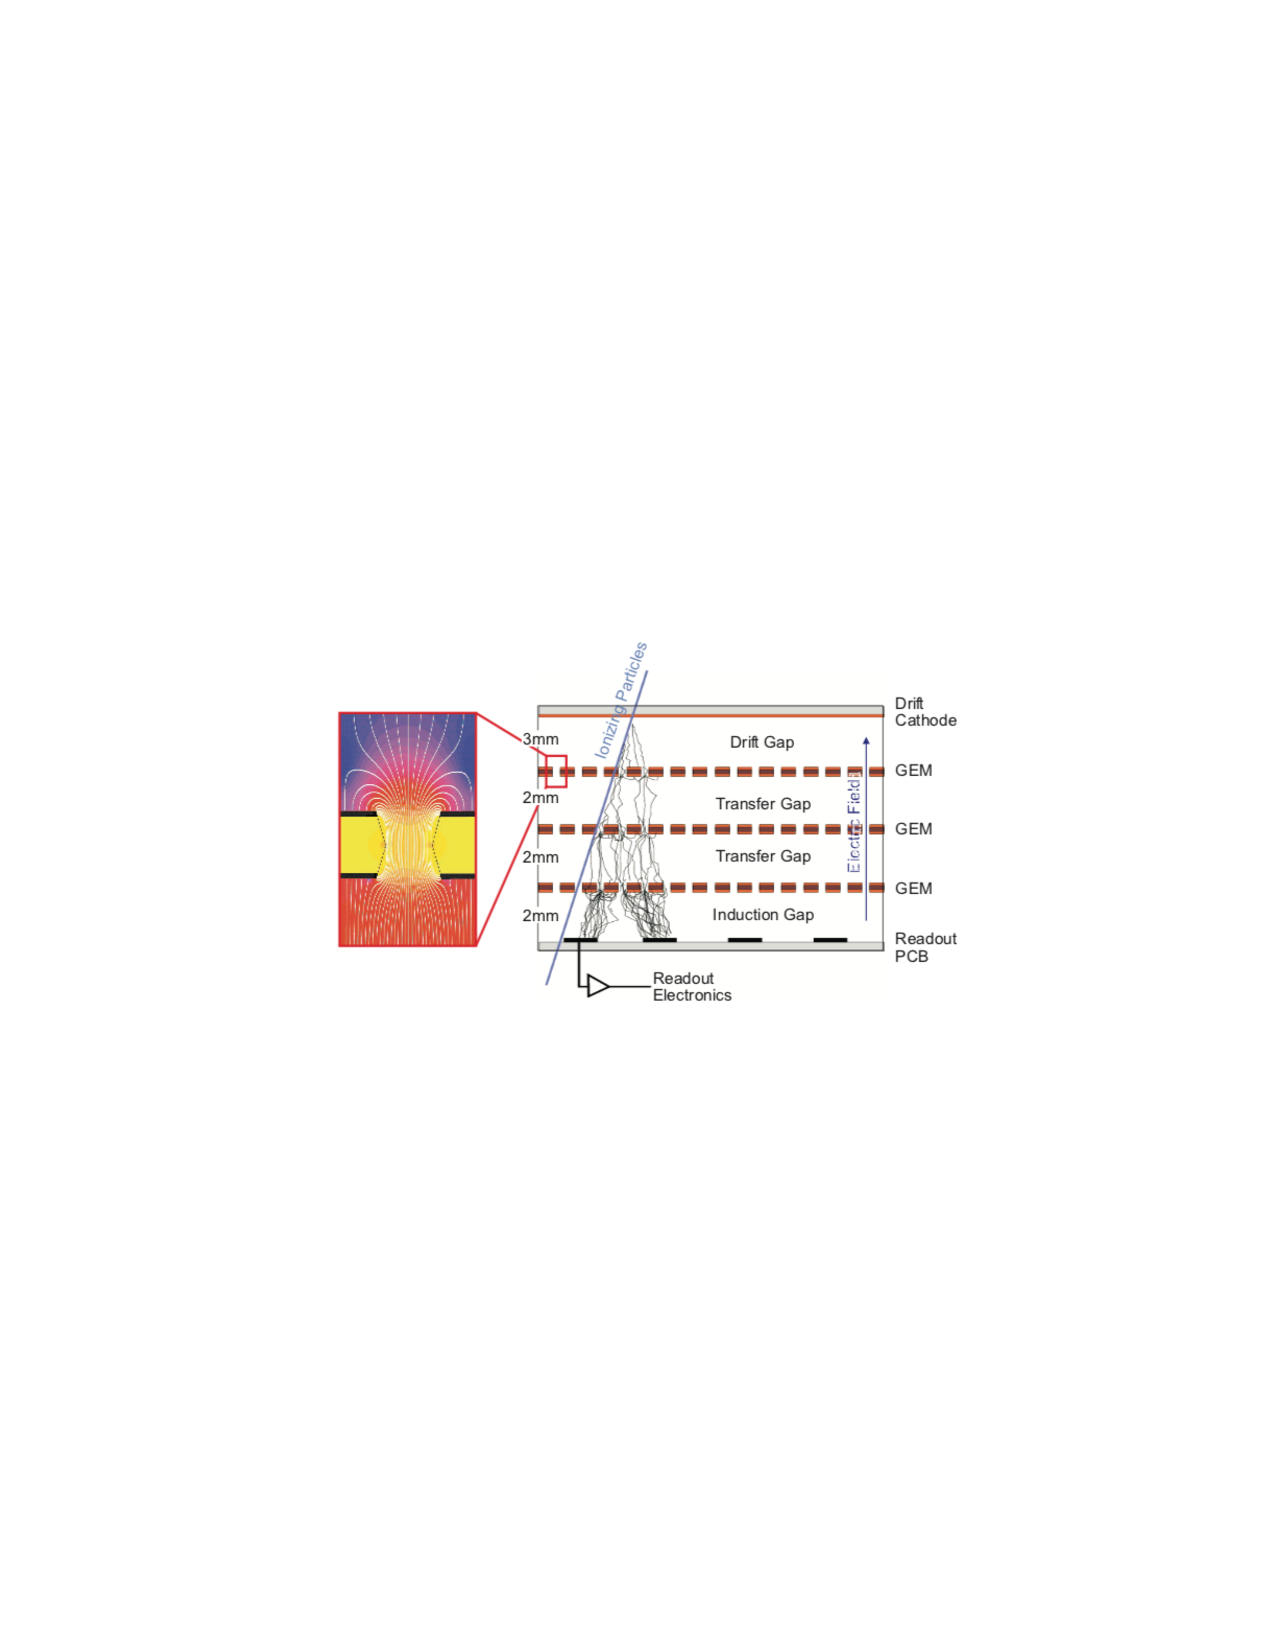
\includegraphics[width=0.7\textwidth,trim=4cm 10cm 4cm 10cm, clip]{GEM}
  \caption{The operation principle of the gas electron multiplier (GEM)
    detectors}
  \label{fig::GEM}
\end{figure}

\subsection{Large Area Trackers}
The large area trackers measure the largest polar scattering angles at COMPASS.
Their dead zones mostly coincide with a small area tracker, described in the
previous section~\ref{sec::SAT}, which therefore means these detectors do not
have to process the higher fluxes very close to the beam line.  The most
important feature of these detectors is that they have a large planar area. As a
consequence however, their position and timing resolutions are not as good as
the small and very small angle trackers.  The types of large area trackers used
at COMPASS are all gaseous detectors and include drift chambers (DCs), straw
tube detectors (straws) and multi-wire proportional chambers (MWPCs). \par

The first four drift chambers downstream of the target are named DC00, DC01,
DC04 and DC05.  The first two, DC00 and DC01, have smaller active areas of
180x127~cm$^2$ and a circular dead zone of 30~cm diameter.  These two drift
chambers are positioned upstream of the SM1 magnet.  The rates upstream of SM1
are higher.  This is due to the fact that low energy particles are produce in
the target, but are bent out of the acceptance of spectrometer by SM1.
Therefore detectors downstream of SM1 do not track these low energy particles
and therefore DC00 and DC01 need to be able to process a higher particle flux.
The next two drift chambers, DC04 and DC05, are downstream of SM1 and both have
larger active areas of 240x204~cm$^2$ and as well have dead zones of 30~cm
diameter.  The active areas of all four of these DCs was roughly chosen to
coincide with the acceptance of the SM1 yoke.  DC05 was first installed for the
2015 Drell-Yan data taking and is further described in chapter~\ref{ch::DC05}.
All four of these DCs measure four projection views corresponding to eight
detector layers.  A sketch of the principle of operation is shown in
Fig.~\ref{fig::DCoperation}.  The nominal spacial resolution for these detectors
is 250~$\mu$m. \par

\begin{figure}[h!t]
  \centering
  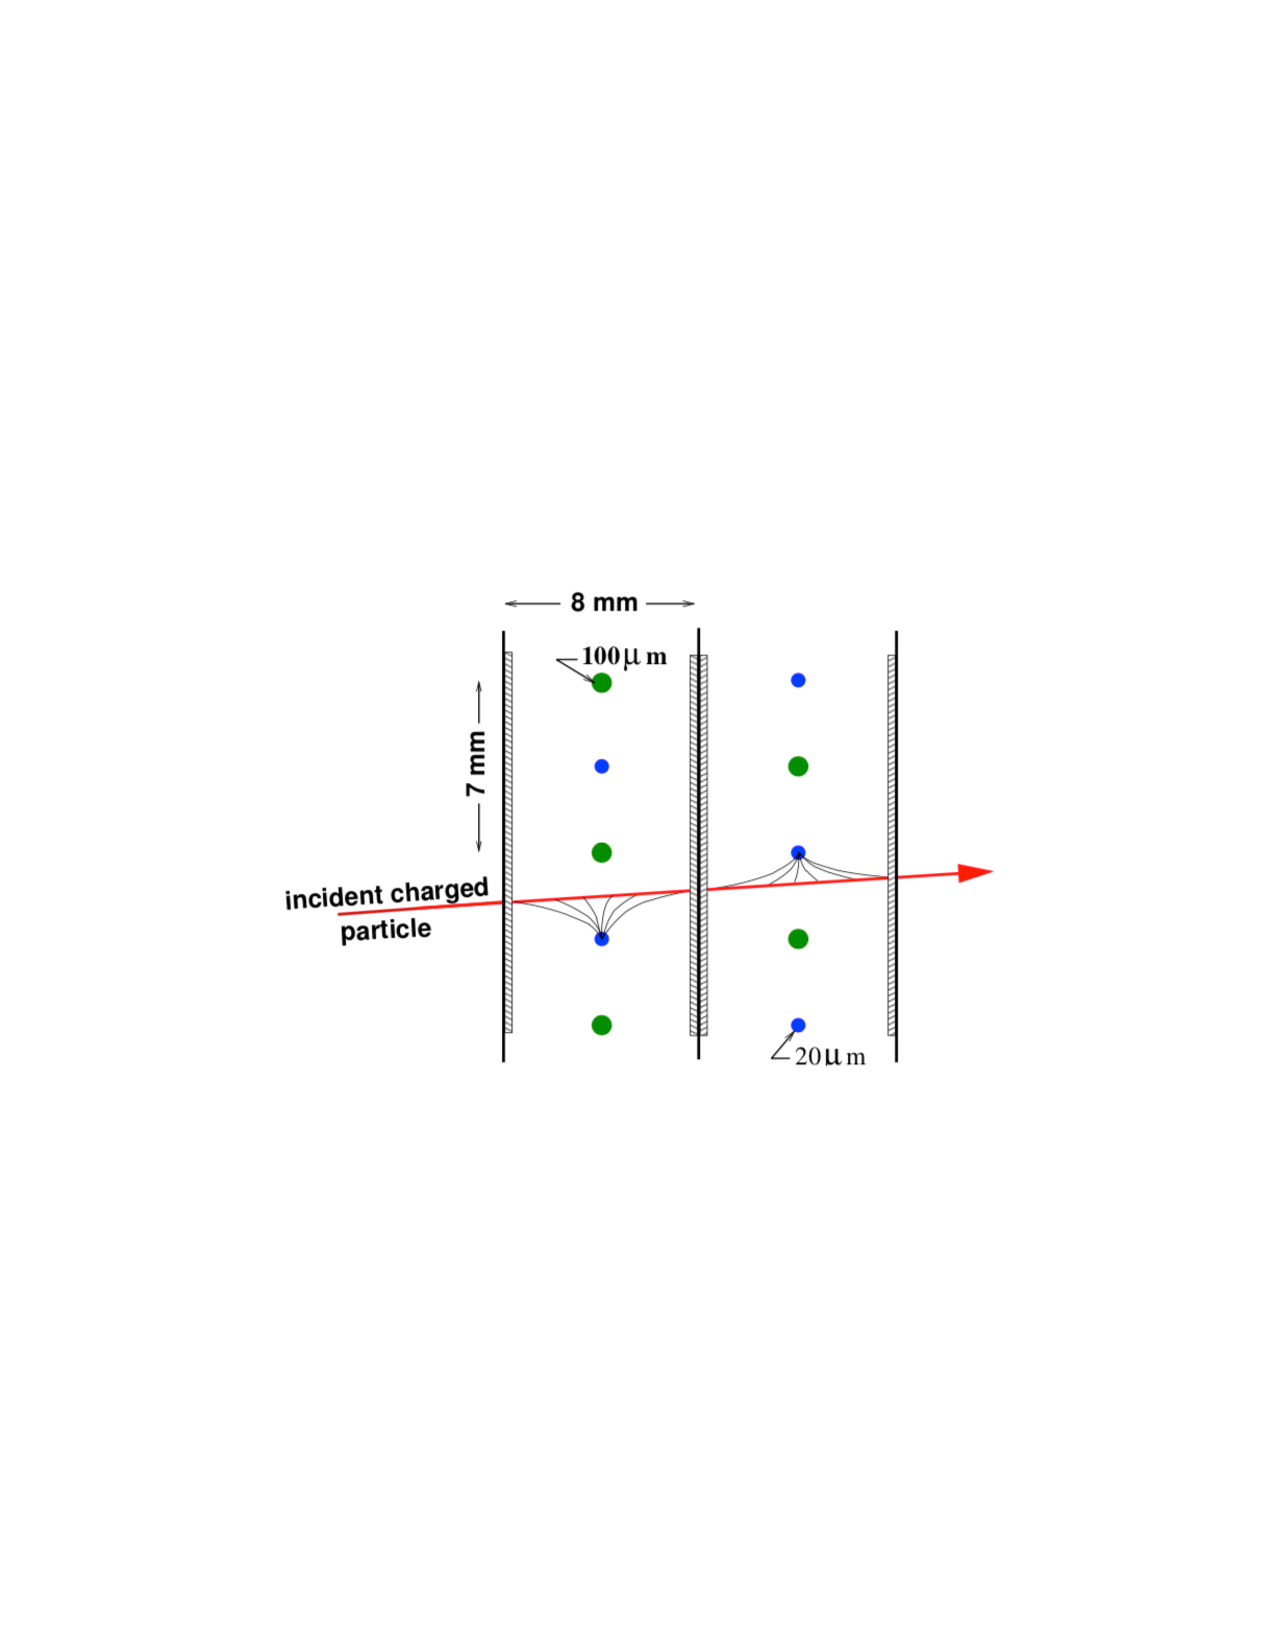
\includegraphics[width=0.6\textwidth,trim=4cm 8cm 4cm 10cm,
    clip=true]{DCoperation}
  \caption{Drift cell of a drift chamber with the ionized drift electron lines
    coming from the incident charged particle}
  \label{fig::DCoperation}
\end{figure}

Further downstream the spectrometer, downstream of the SM2 magnet, are the W45
drift chamber stations.  The W45 drift chambers are the largest drift chambers
at COMPASS.  There are six W45 detector stations which each have an active area
of 520x260~cm$^2$ and a circular dead zone of 50~cm or 100~cm diameter.  Each
W45 station measures two projection views corresponding to four detector layers.
The drift cells in W45 are 40x10~mm$^2$ and the spacial resolution is nominally
1500~$\mu$m. \par

The two straw stations in operation during the 2015 data taking are named ST03
and ST05.  ST03 was in the large angle spectrometer after DC05 and consisted of
two stations measuring six projection views.  ST05 was in the small angle
spectrometer and measured three projection views.  The active areas of each of
the horizontal wire stations is 350x243~cm$^2$ and the active area of each of
the rotated wires is 323x272~cm$^2$.  The principle of operation for the straw
detectors is very similar to that of a drift chamber.  However, instead of
having the detector made up of connected drift cells the straw detectors are
made of separated circular tubes.  Each tube consist of a gold plated tungsten
anode wire in the center and the walls of the tube make up a cathode.  Due to
the fact that the cathode completely surrounds the anode wire there is no
electrical interference between neighboring anode wires as there is for drift
chambers.  For this reason the electric field in each tube is easier to control
and the ionized electron drift speed is more linear than other detectors.  Each
straw detector plane is divided into sections where the straw tubes in the outer
most section from the beam line have a diameter of 9.6~mm and the tubes close to
the beam line have a diameter of 6.1~mm.  In addition, in the central part of
the detector there is a physical hole, dead zone of 20x20~cm$^2$.  The nominal
position resolution for these detectors is 400~$\mu$m.  A frontal schematic is
shown in Fig.~\ref{fig::frontalStraw}.  For the reason that most of the detected
muons are reconstructed in the large angle spectrometer and the fact that many
of the high voltage modules were not operation for ST05 in 2015, ST05 was not
used for track reconstruction for 2015 Drell-Yan data. \par

\begin{figure}[h!t]
  \centering
  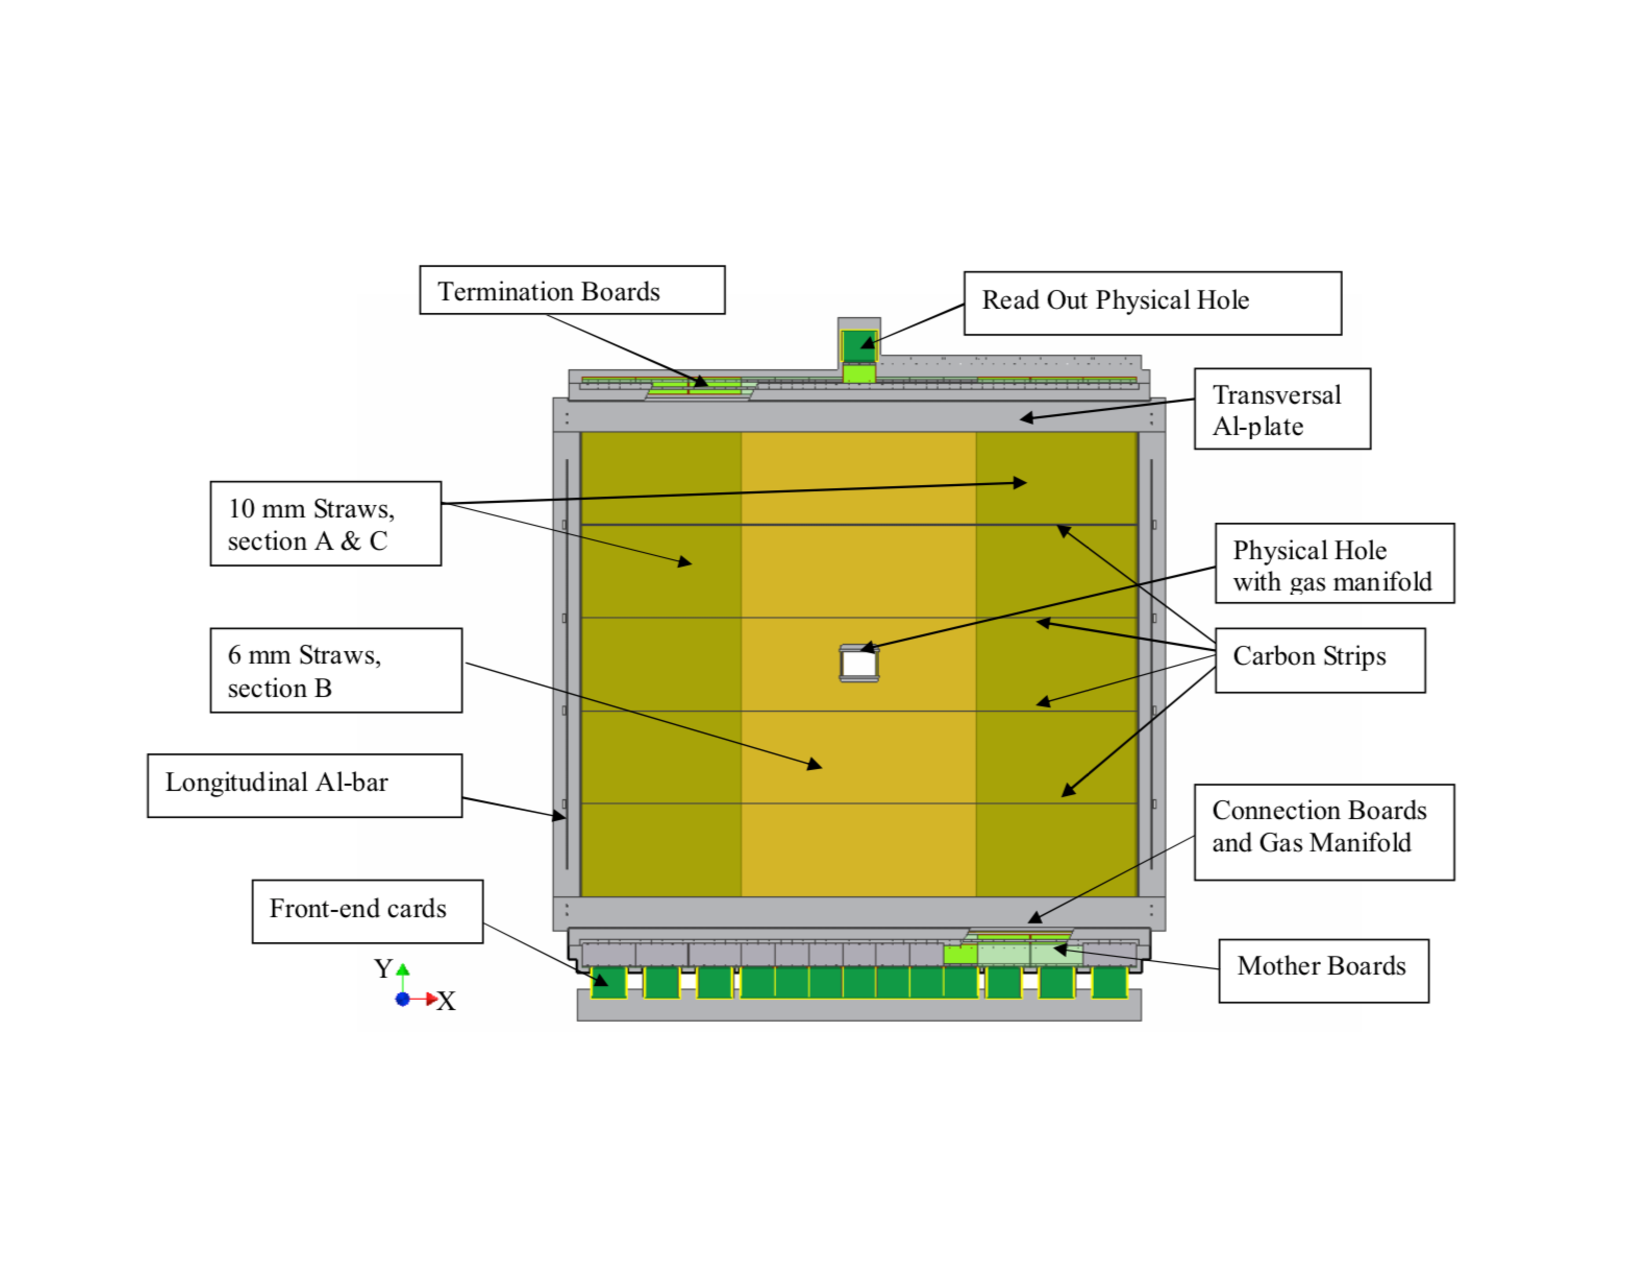
\includegraphics[width=0.8\textwidth,trim=2cm 4cm 3cm 4cm,clip]{frontalStraw}
  \caption{Front on view of a the active area of a straw detector at COMPASS}
  \label{fig::frontalStraw}
\end{figure}

The next type of large angle track is the richwall.  This large area tracker
operates similarly to the straw tube detectors.  The detector consist of eight
layers of mini drift tubes (MDT) shown in Fig.~\ref{fig::richwallMDT}.  The
central part of each MDT includes a gold plated tungsten sense wire.  The
richwall is located before the SM2 magnet and after ST03 with an active area of
5.27x3.91~cm$^2$ and a central dead zone of 1.02x0.51~cm$^2$.  The nominal
position resolution of this detector is 600~$\mu$m. \par

\begin{figure}[h!t]
  \centering
  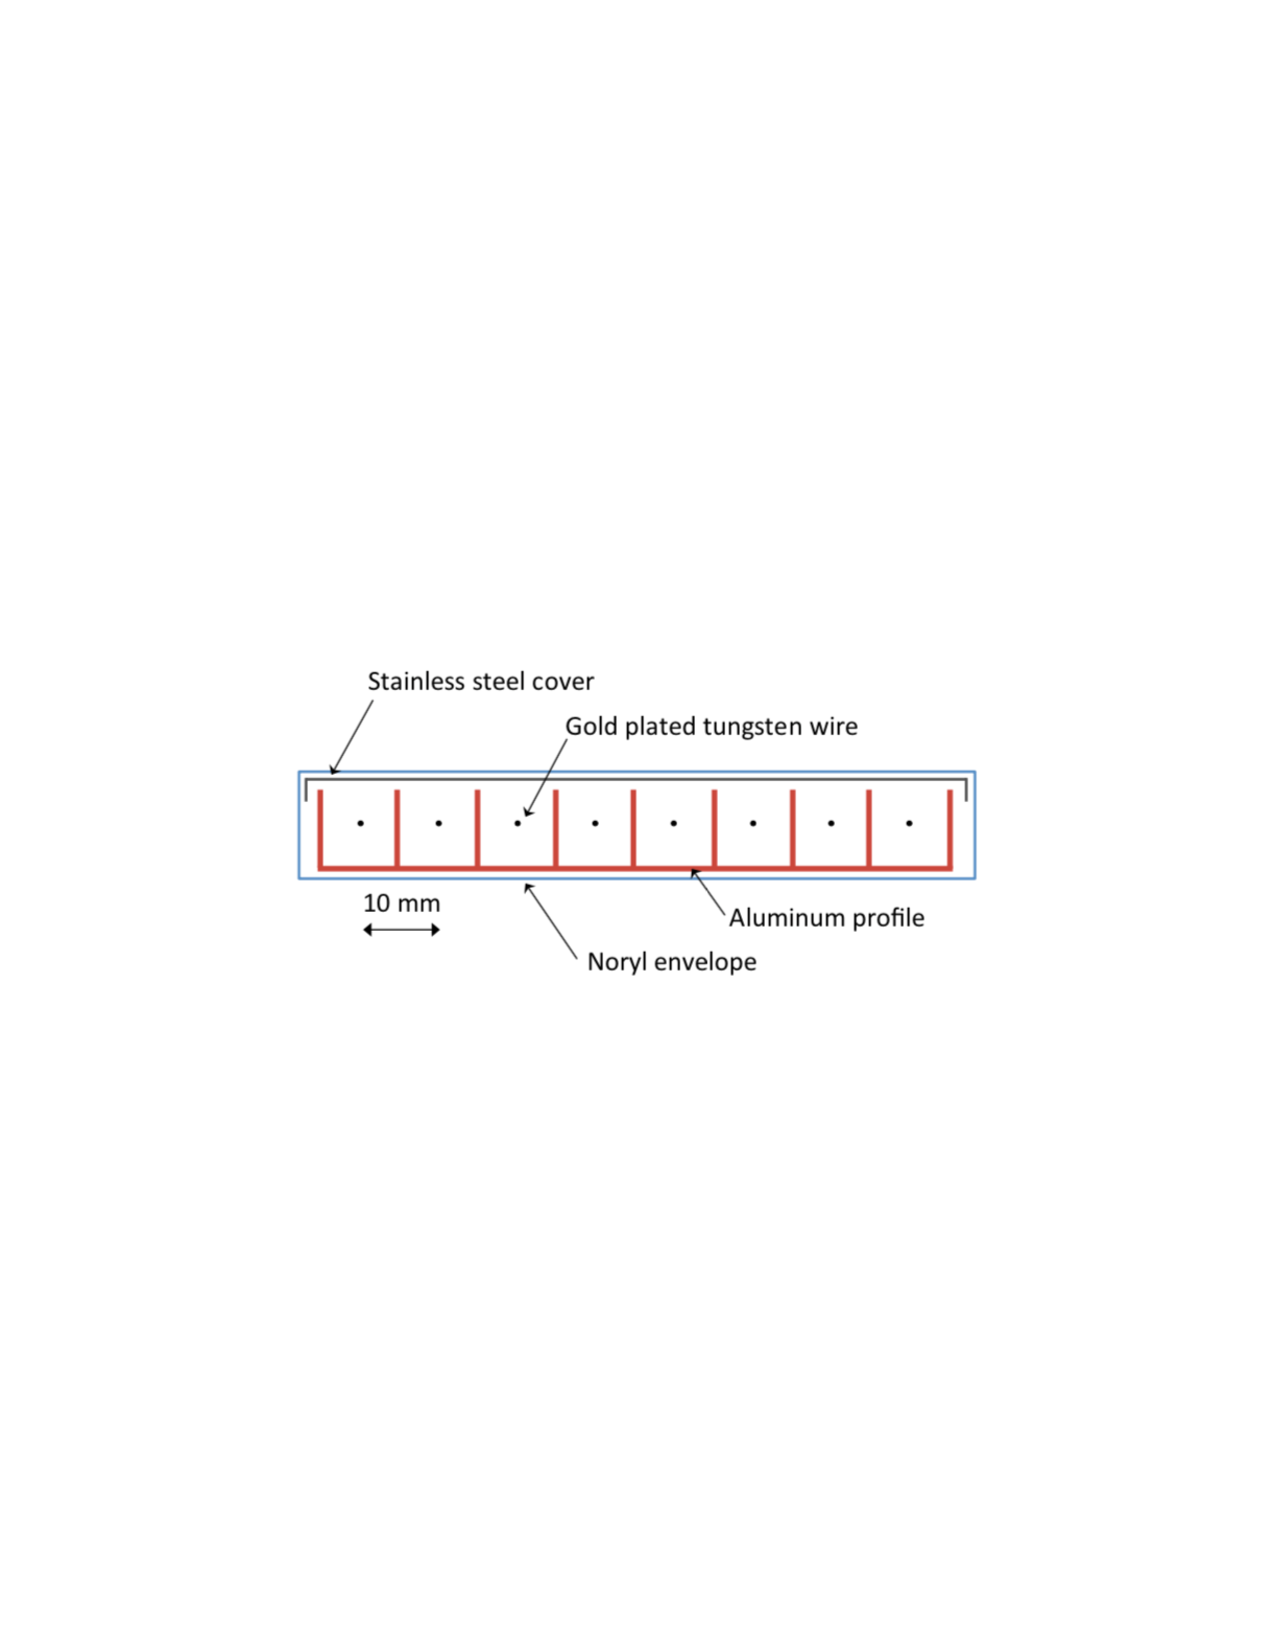
\includegraphics[width=0.45\textwidth, trim=5cm 12cm 5cm 10cm, clip]
                  {richwallMDT}
  \caption{The richwall mini drift tubes}
  \label{fig::richwallMDT}
\end{figure}

The final type of large area tracking detector at COMPASS is the MWPC.  There
are 14 of these stations located throughout the experiment.  The MWPCs are
separated into three categories distinguished by the coordinates they measure.
The first type is called type A and consists of three projection views measuring
an x, u and v coordinate.  The second type is type A* and is the same as type A
but measures the y coordinate in addition to the other three coordinates.  Both
type A and A* have active areas of 178x120~cm$^2$.  The final type is type B
which has a smaller active area of 178x90~cm$^2$ and measures the same
projections as type A.  There are seven stations of type A, one station of type
A* and six stations of type B.  All three types have circular dead zones of
diameters 16~cm, 20~cm and 22~cm for types A, A* and B respectively. \par

The MWPCs operate on similar principles to the drift chambers but without a
calibration drift curve.  For this reason the MWPCs can be made to have one
common gas volume between each station.  Their position resolution is
determined as

\begin{equation}
\frac{\mathrm{sense \: wire \: separation}}{\sqrt{12}},
\end{equation}
\noindent
which is the variance of a uniform distribution.  The separation between sense
wires is approximately 2~mm which corresponds to a spacial resolution of these
detectors of around 600~$\mu$m.


\section{Particle Identification}
In the COMPASS spectrometer there are four types of detectors used to determine
particle identification (PID).  These four detectors are the ring image
Cherenkov (RICH) detector, electromagnet calorimeters (ECAL), hadron
calorimeters (HCAL) and muon walls (MW).  The RICH distinguishes between pions,
kaons and protons; ECAL1 and ECAL2 measure the energy from photons and
electrons; HCAL1 and HCAL2 measure the energy from hadrons; and MW1 and MW2
distinguish muons from all other particles.  The RICH, ECAL1, HCAL1 and MW1 are
in the large angle spectrometer in that respective order along the beam line.
The small angle spectrometer includes ECAL2, HCAL2 and MW2 again in that
respective order along the beam line. \par

The RICH detector operates similarly to the CEDARS, section~\ref{sec::addBeam}.
In the RICH, Cherenkov radiation is emitted from particles traveling through it
at an angle dependent on the particle's velocity.  The RICH is filled with a
dielectric gas, C$_4$F$_{10}$, which as an index of refraction greater than air.
The momentum of a particle going through the RICH is determine from bending
radius around SM1.  Therefore once the RICH determines the entering particles
velocity, the mass of particles can be distinguish.  A sketch of the RICH and
its operating principle is shown in Fig.~\ref{fig::rich}.  To distinguish
between particles the minimums momentums are: 2.5~{\gvc} for pions, 9~{\gvc} for
kaons and 17~{\gvc} for protons.  The maximum momentum the RICH can distinguish
between any of these particles is 50~{\gvc}. This detector is located in the
large angle spectrometer before any calorimeters.\par

\begin{figure}[h!t]
  \centering
  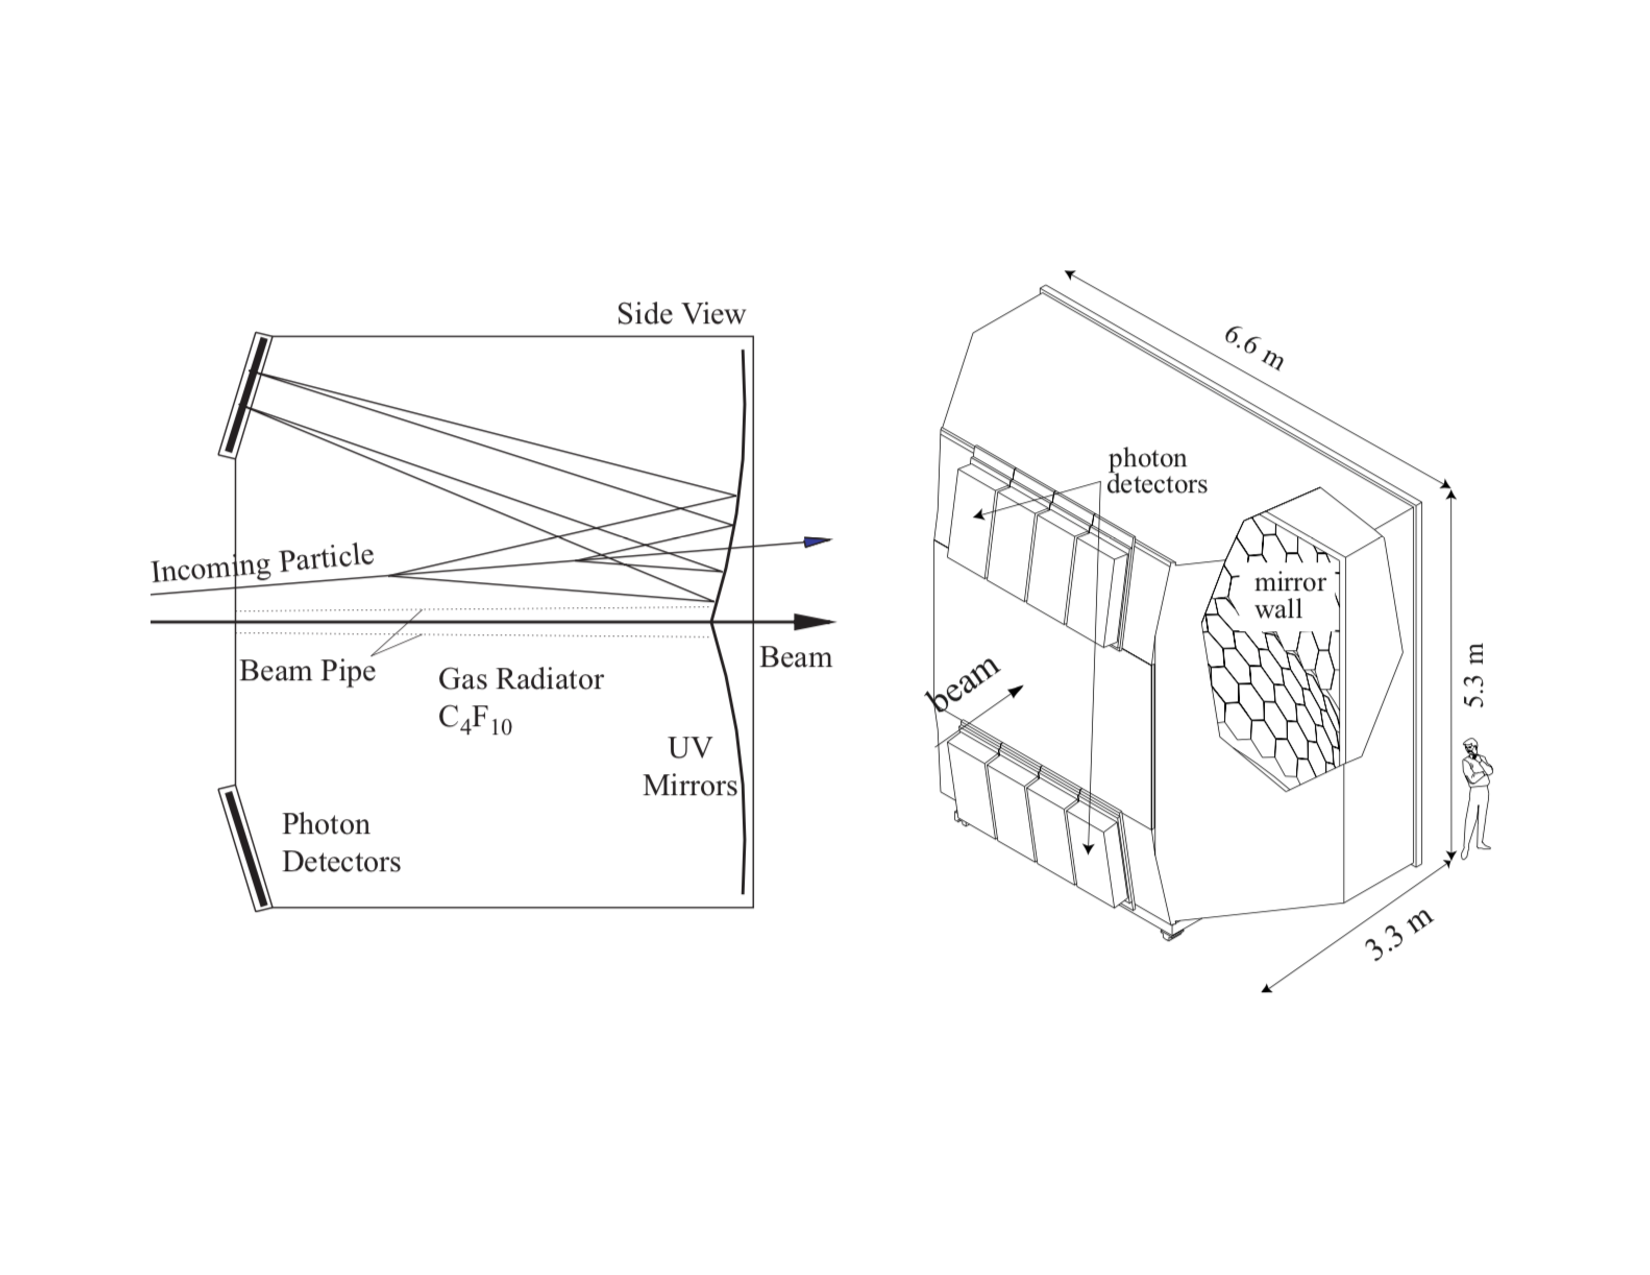
\includegraphics[width=0.6\textwidth, trim=1cm 5cm 1cm 4cm, clip]{rich}
  \caption{Side view demonstrating the principle of operation of the RICH
    detector.}
  \label{fig::rich}
\end{figure}

The ECALs and HCALs both measure the energy of entering particles.  Both types
of calorimeters do this by stopping a specific entering particle, where the
amount of energy deposited in each respective calorimeter is proportional to the
incoming particle's energy.  ECALs are able to stop and measure electron and
photon energies and HCALs stop and measure hadron energies.  The energy
knowledge along the momentum determined from the tracking detectors allows the
ability to determine the particle's identification. \par

The ECALs are made of lead glass towers with photon multipliers attached to
these towers on one side.  An incoming photon or electron interacts with the
lead glass to produce a light signal which is readout with these photon
multipliers.  Other particles also interact with the material in the ECALs
however hadrons and muons are able to exit through the detector unlike photons
and electrons.  A frontal view of ECAL1 is shown in Fig.~\ref{fig::ECAL1} and a
frontal view of ECAL2 is shown in figure Fig.~\ref{fig::ECAL2}. \par

\begin{figure}[h!t]
  \centering
  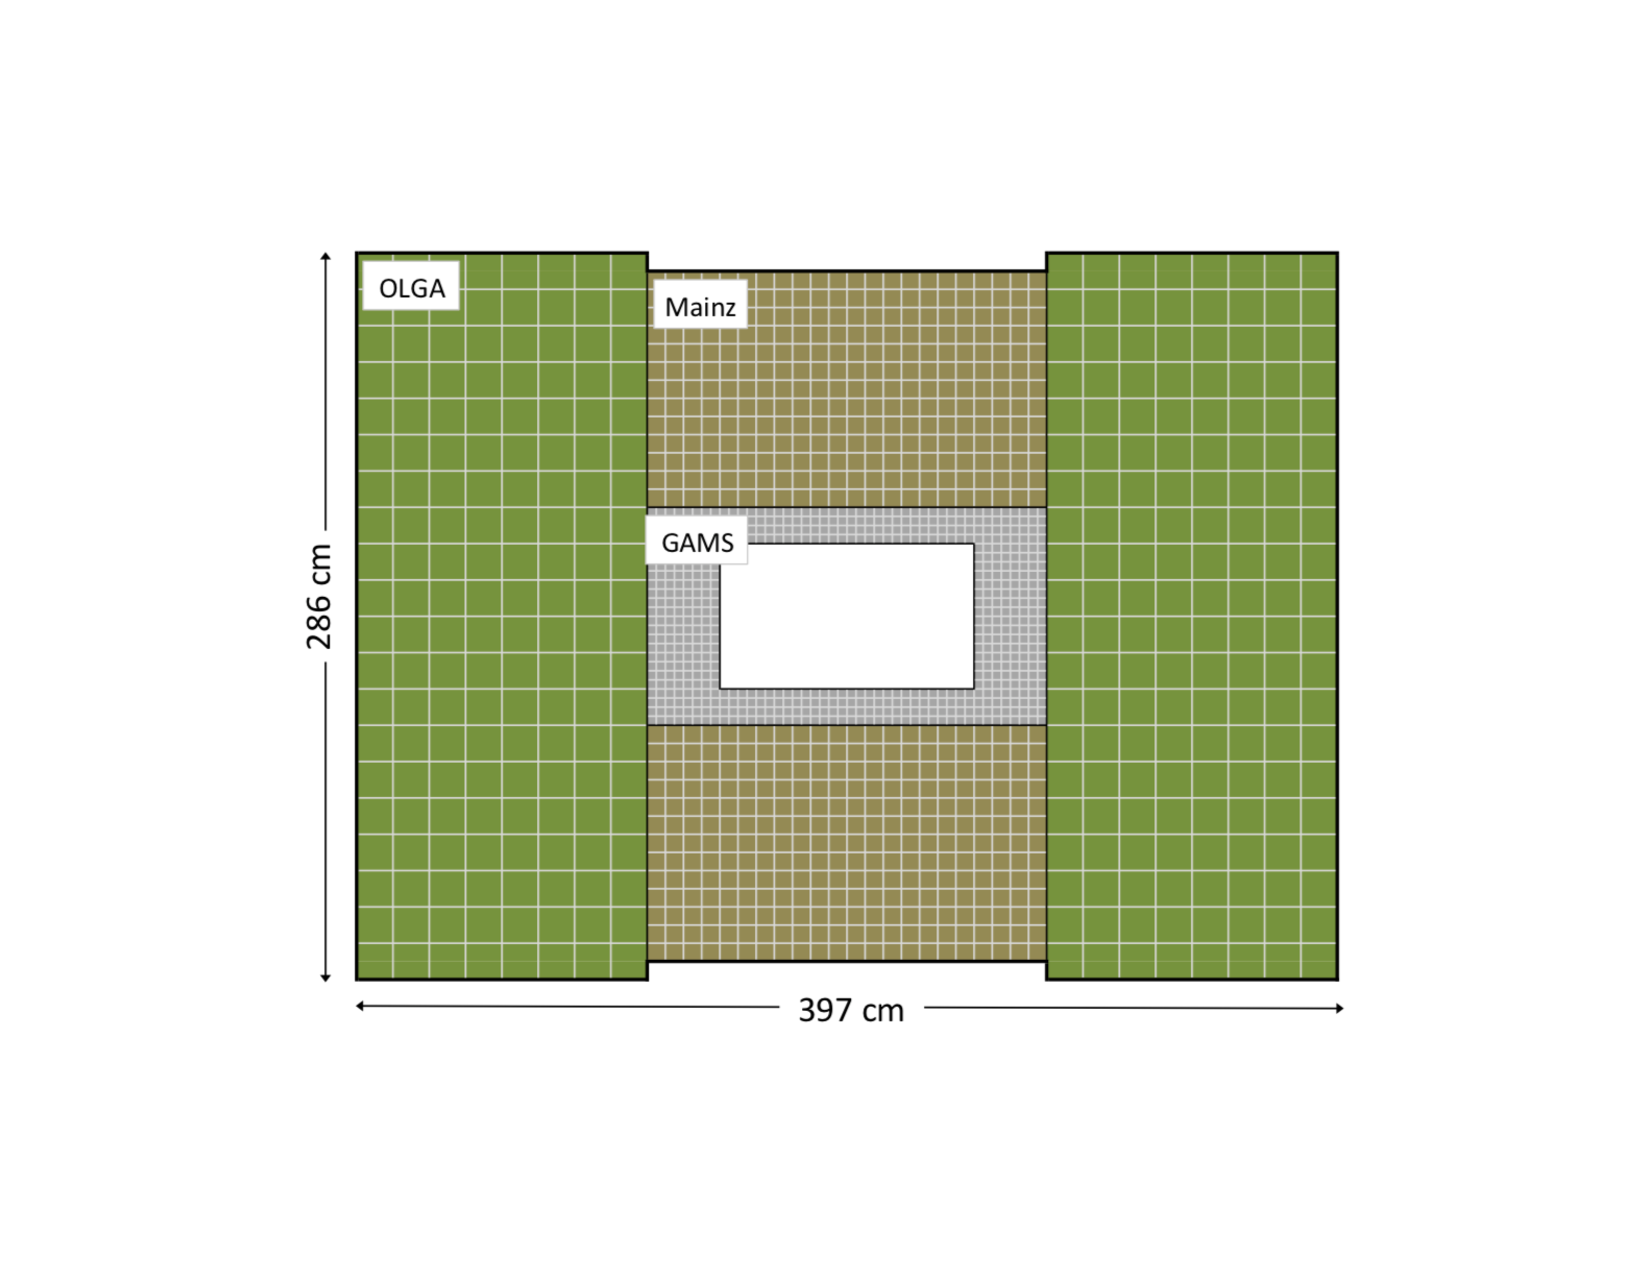
\includegraphics[width=0.6\textwidth, trim=4cm 4cm 4cm 4cm,clip]{ECAL1}
  \caption{Frontal view of the electromagnetic calorimeter 1}
  \label{fig::ECAL1}
\end{figure}

\begin{figure}[h!t]
  \centering
  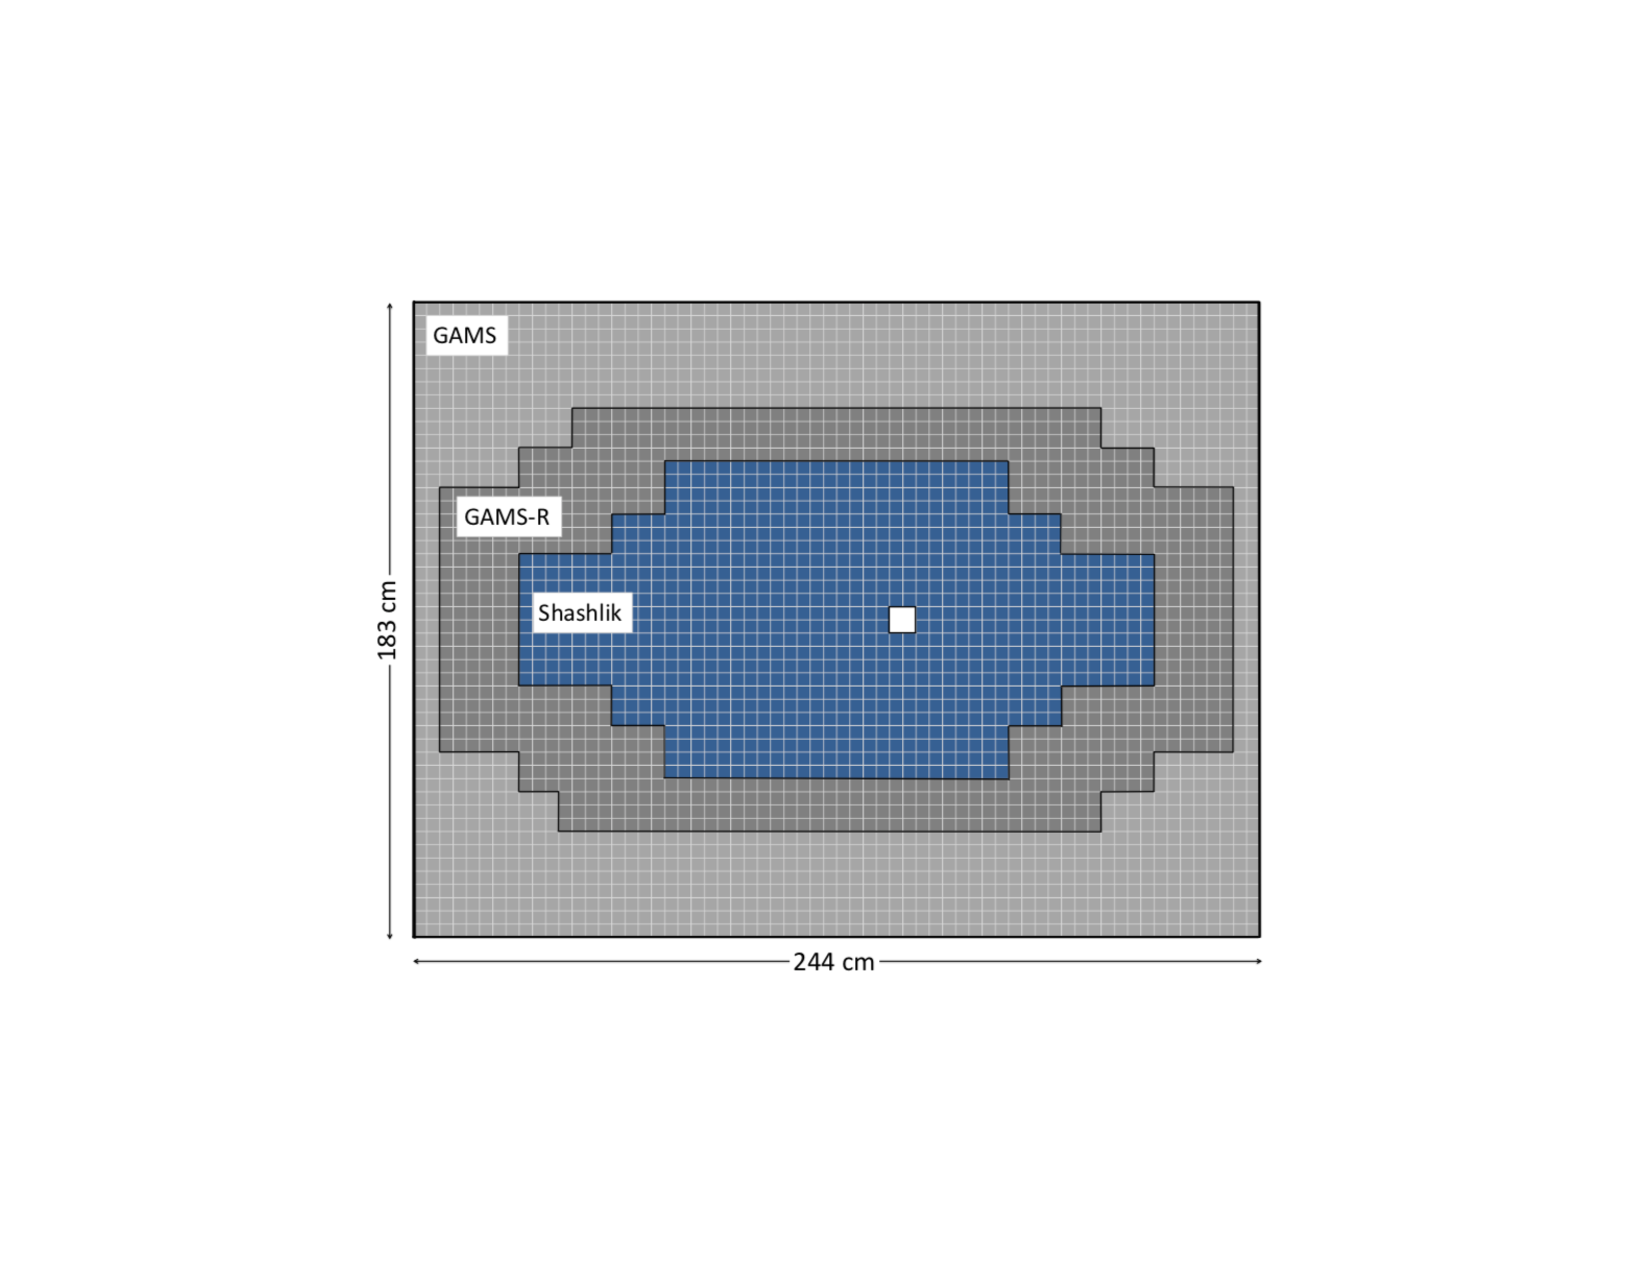
\includegraphics[width=0.6\textwidth, trim=4cm 4cm 4cm 4cm,clip]{ECAL2}
  \caption{Frontal view of the electromagnetic calorimeter 2}
  \label{fig::ECAL2}
\end{figure}


The HCALs are sampling calorimeters which are made of alternating layers of iron
and scintillating material.  An incoming hadron deposits all its energy in the
HCAL by making a particle showers in the iron.  This particle shower makes a
signal in the scintillating material which is then read out by photo
multipliers.  The HCALs are placed after the ECALs in each stage of the
spectrometer because an electromagnetic shower happens within less material
budget than a hadronic shower.  The HCALs are effect at determining particle
energies from particle with energies between 10~GeV and 100~GeV. \par

The two MWs are located after an HCAL in their respective stages.  Due to their
higher mass and absence of color charge, muons are able to pass through the most
material budget of any of the particles detected at COMPASS.  For this reason
both MWs consist of an absorber and tracking detectors downstream of this
absorber.  Any particles that make it through the absorber are with a very high
probability muons. \par

MW1 consists of eight tracking planes before a 60~cm iron
absorber and the same number of tracking planes after this absorber.  The
tracking portions of MW1 are built similarly to the richwall, described in
section~\ref{sec::SAT}, in that they are also made of MDT modules.  The active
area of MW1 is 480x410~cm$^2$ and includes a dead zone of 140x80~cm$^2$.  Each
plane of this detector has a spacial resolution of 3~mm.  A sketch of MW1 is
shown in Fig.~\ref{fig::MW1}. \par

\begin{figure}[h!t]
  \centering
  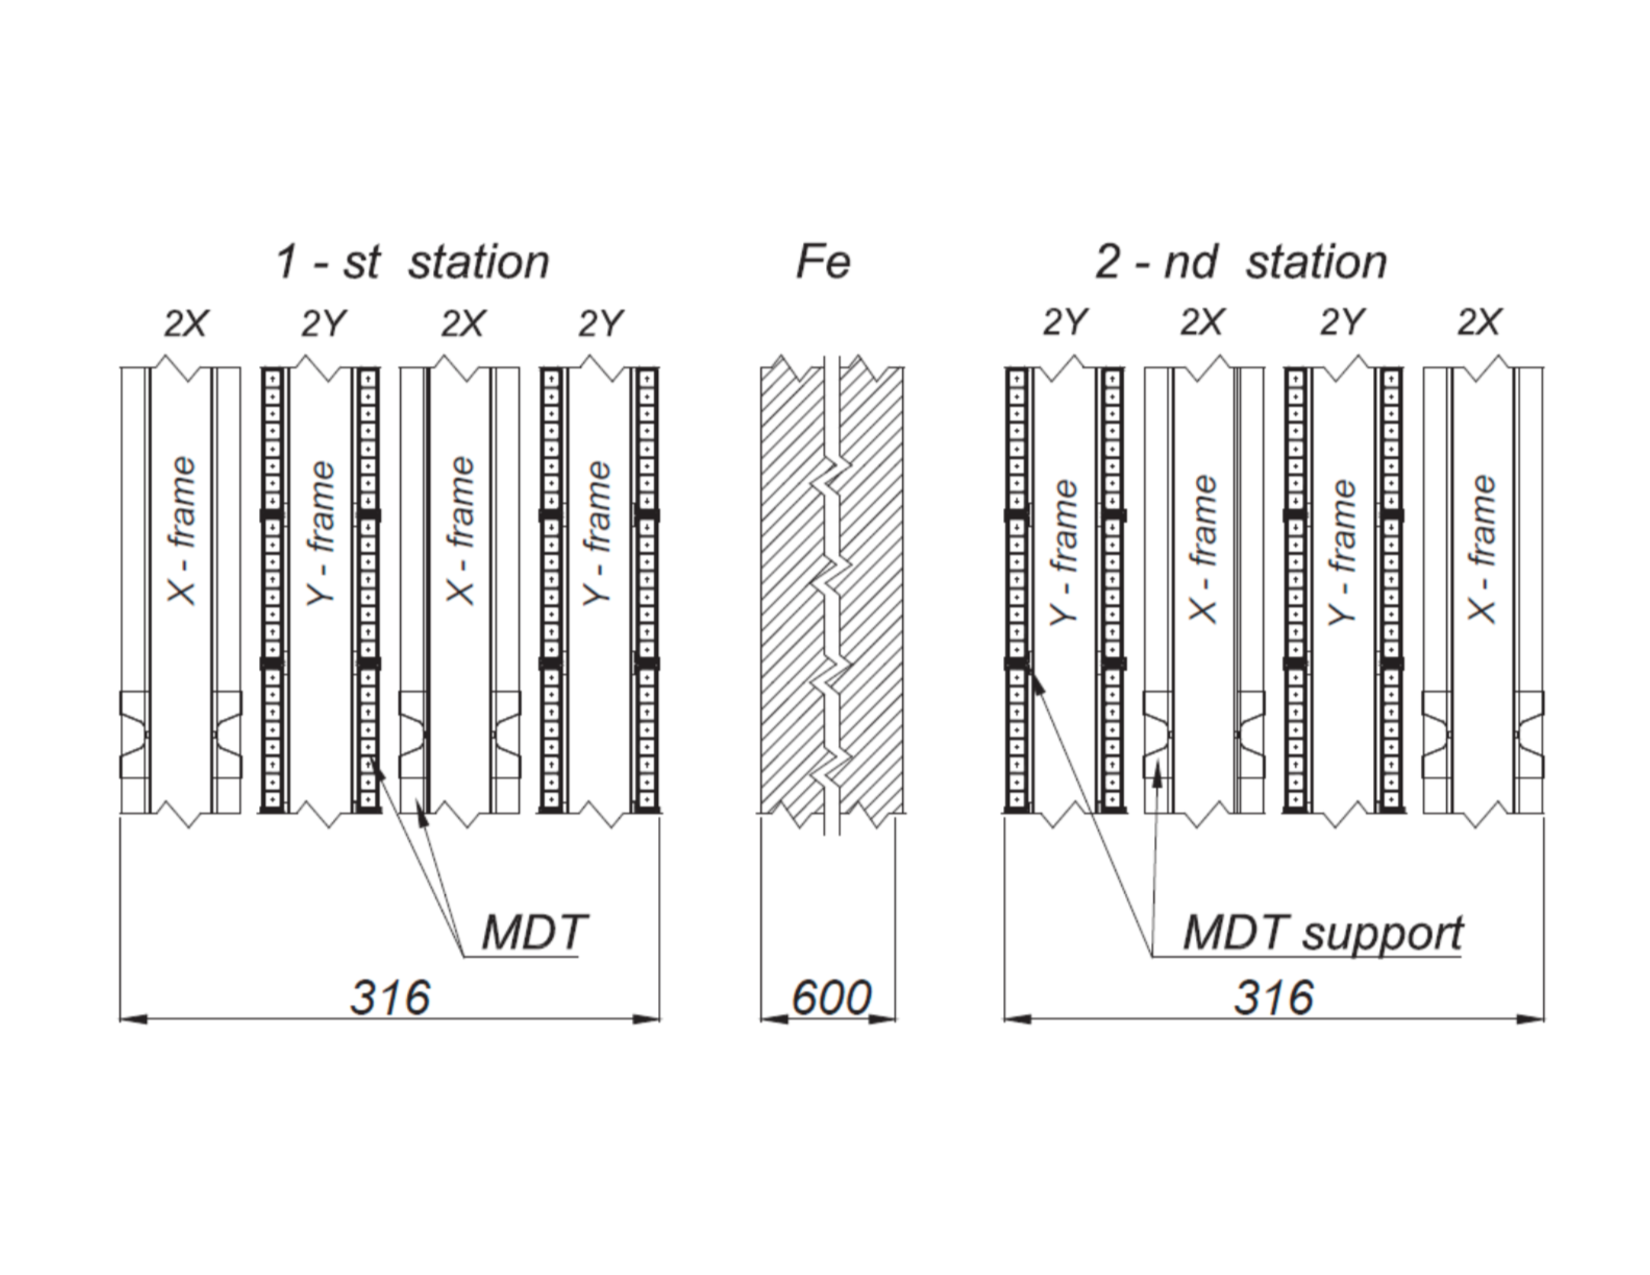
\includegraphics[width=0.7\textwidth, trim=1cm 3cm 1cm 3cm,clip]{MW1}
  \caption{A side view sketch of the muon wall 1 detector}
  \label{fig::MW1}
\end{figure}

The second muon wall, MW2, is located downstream of a 2.4~m thick concrete
absorber.  MW2 consists of 12 planes each with an active area of 450x450~cm$^2$
and a dead zone of 90x70~cm$^2$.  The detector operates similarly to the straw
detectors, section~\ref{sec::SAT}, in that the detector is made of drift tubes
with a wire in the center of these tubes.  The diameter of the drift tubes is
29~mm and the position resolution is about 1.4~mm. \par

There is one last absorber in the COMPASS spectrometer located before the H5
hodoscope at the end of the spectrometer hall.  This absorber is called muon
filter 3 (MW3) and ensures that the inner trigger is only triggered by a
muon. \par


\section{Trigger}
The trigger system at COMPASS defines what is an event.  Whenever the trigger
signal is given, all the detector information within a few nanosecond timing
window is recorded.  Due to the fact that there are very many background events
occurring as the beam impinges on the target, there is too much information
going to the front end modules (FEMs) of the detectors for the FEMs to process
and record all this information.  For this reason only a certain subset of all
the information is stored to disk.  The trigger system must therefore have good
timing resolution to make quick decisions on which data to record.  At COMPASS
the trigger systems consist of scintillating hodoscopes attached to PMTs.  The
timing resolution of these detectors is approximately 1~ns.  A top view
schematic of COMPASS showing where the relative positions of the hodoscopes for
each trigger is shown in Fig.~\ref{fig::TriggerElements}.  \par

\begin{figure}[h!t]
  \centering
  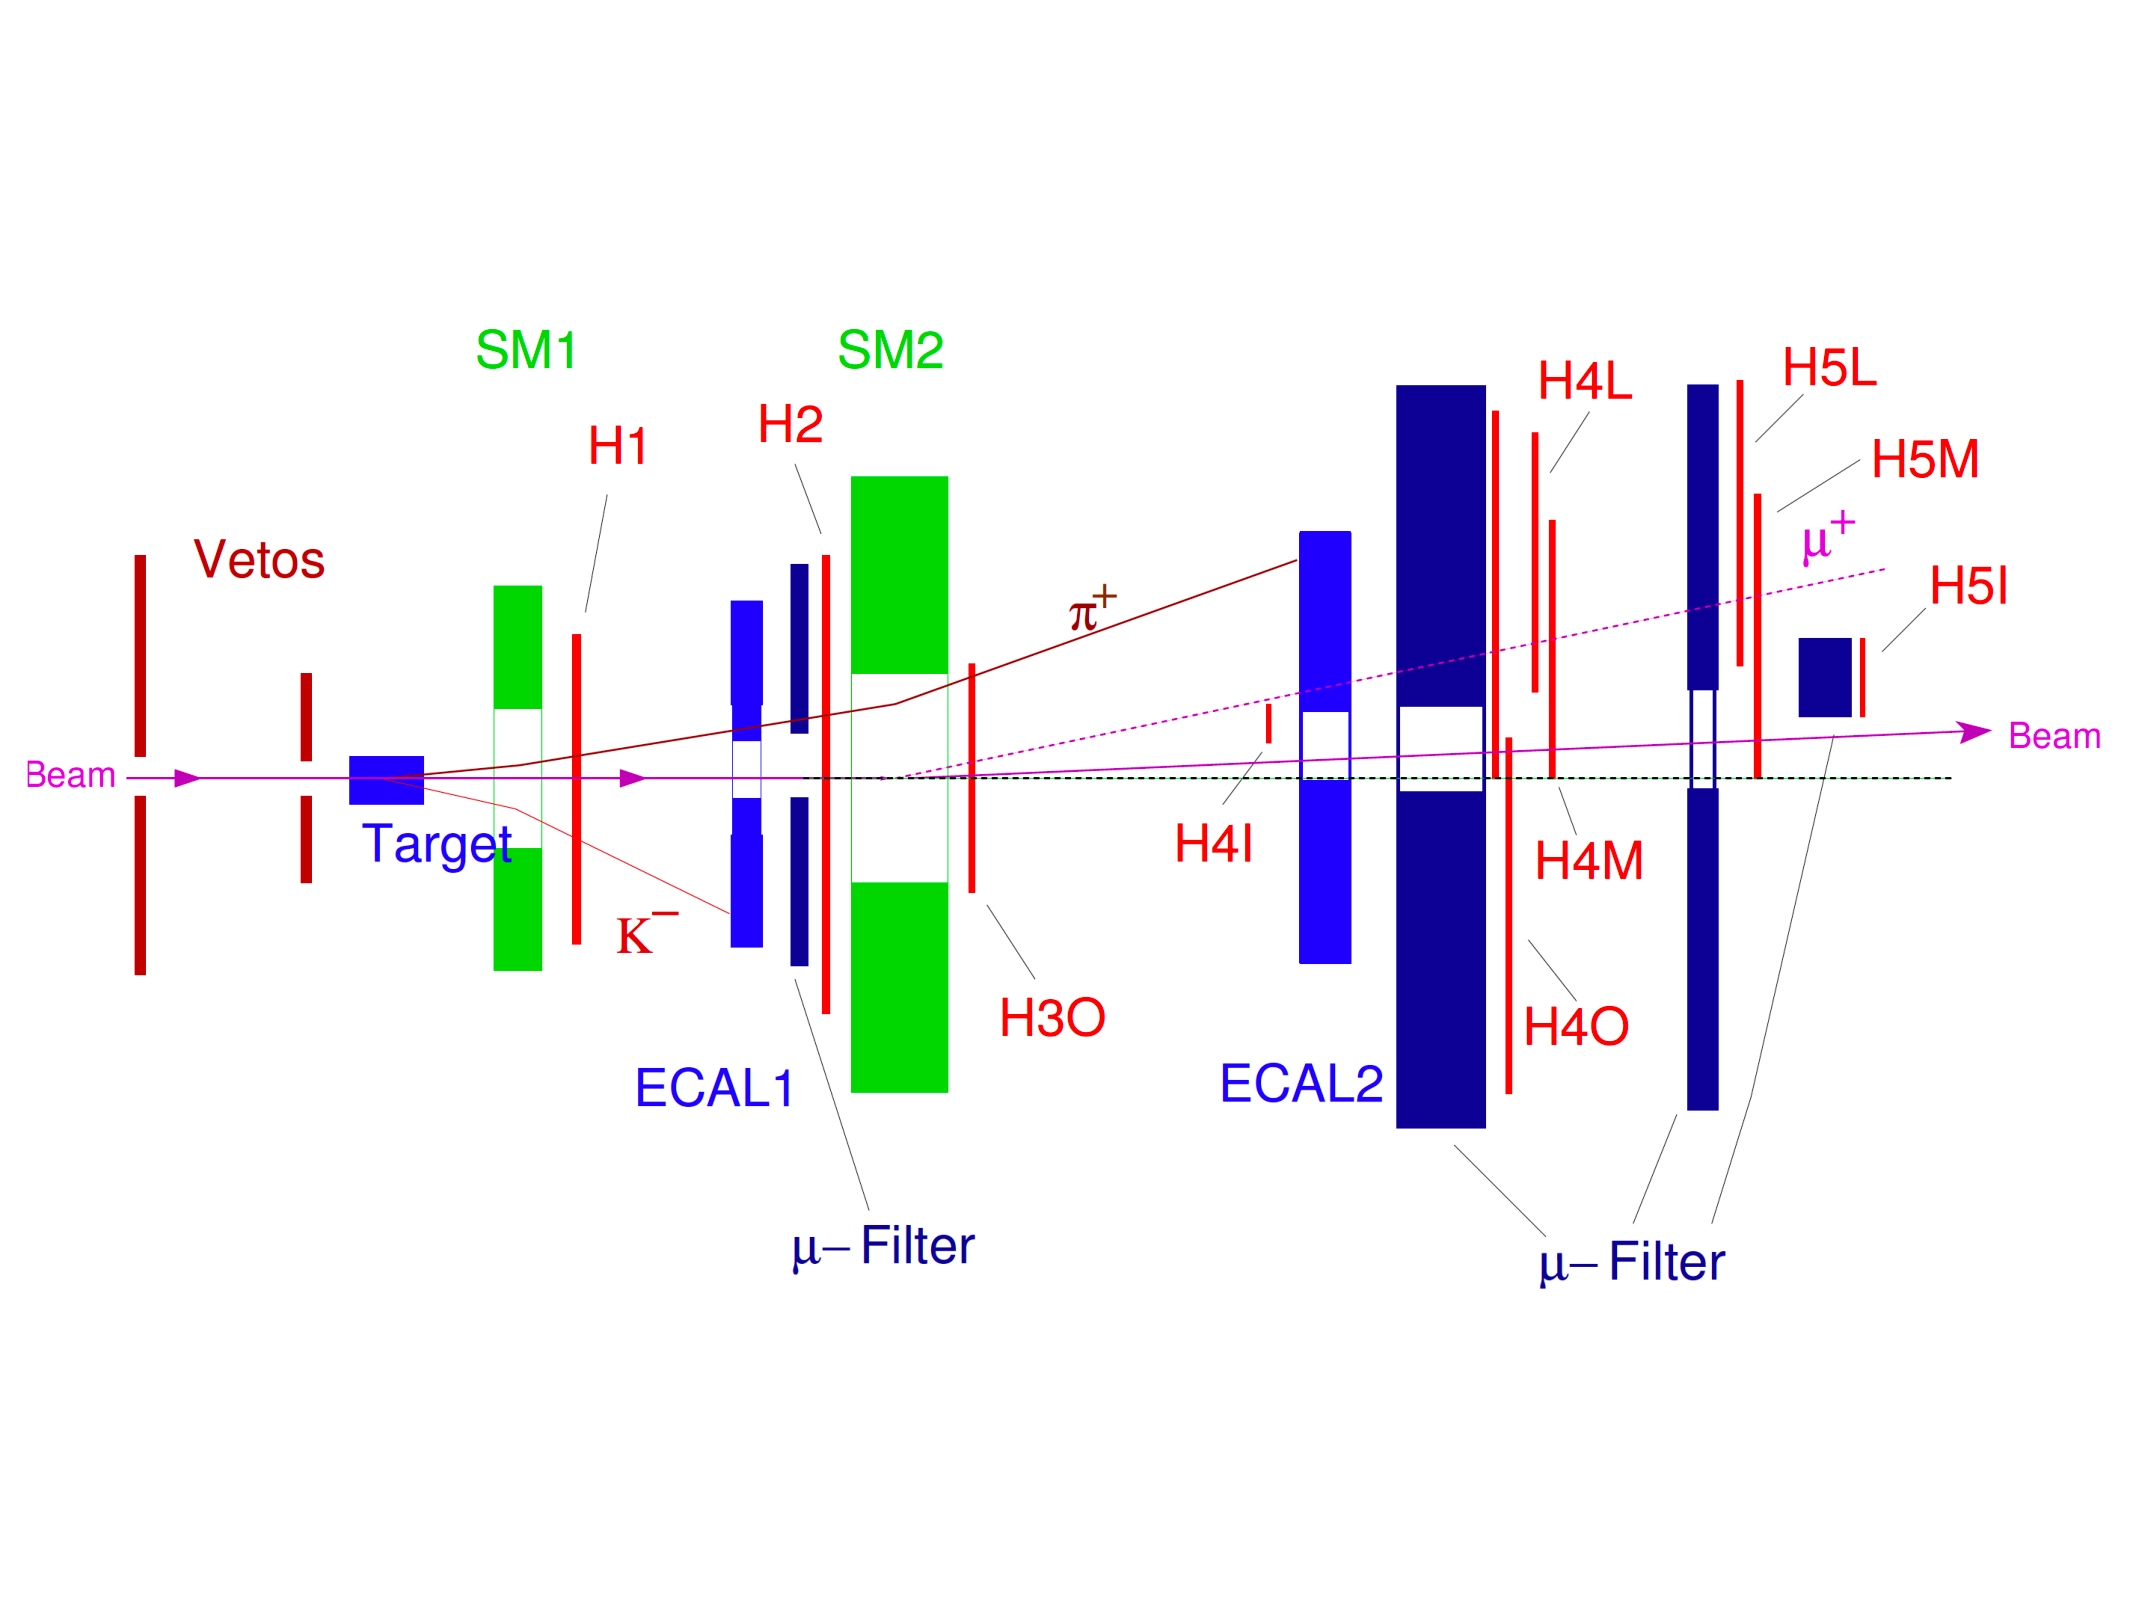
\includegraphics[width=0.9\textwidth]{TriggerElements}
  \caption{Top view of the spectrometer highlighting how different particles can
    signal a trigger}
  \label{fig::TriggerElements}
\end{figure}

At COMPASS there are five different triggers used to register physics events.
Each trigger type includes at least two hodoscopes at different z-positions in
the spectrometer.  The types of triggers are either target pointing, when the
hodoscope slabs are horizontal; or energy loss, when the hodoscope slabs are
vertical.  The target pointing trigger is setup and used with higher polar
scattering angles.  As the name suggest, this trigger signals when a particle is
scattered from the target.  The energy loss trigger is used to trigger on lower
Q$^2$ interactions and signals when a particle is bent a specified amount.
This concept is illustrated in Fig.~\ref{fig::TrigPrinc}.  \par

There are four triggers in SAS: the inner trigger (IT), the middle trigger (MT),
the ladder trigger (LT) and the outer trigger (OT).  The IT is an energy loss
trigger and includes the hodoscopes HI04X and HI05X.  The MT includes both
energy loss and target pointing slabs.  The hodoscopes in the MT are HM04X,
HM05X, HM04Y and HM05Y.  The MT hodoscopes whose names end with an X have
vertical slabs and those ending with a Y have horizontal slabs.  The LT is an
energy loss trigger which consists of HL04X and HL05X.  The final trigger in
SAS, the OT, is a target pointing trigger and consists of hodoscopes HO03Y and
HO04Y.  The remaining trigger system is in LAS and is a target pointing trigger
consisting of hodoscopes HG01Y and HG02Y.  The kinematic coverage for the 2015
triggers is shown in Fig.~\ref{fig::TrigCov6}. \par

\begin{figure}[h!t]
  \centering
  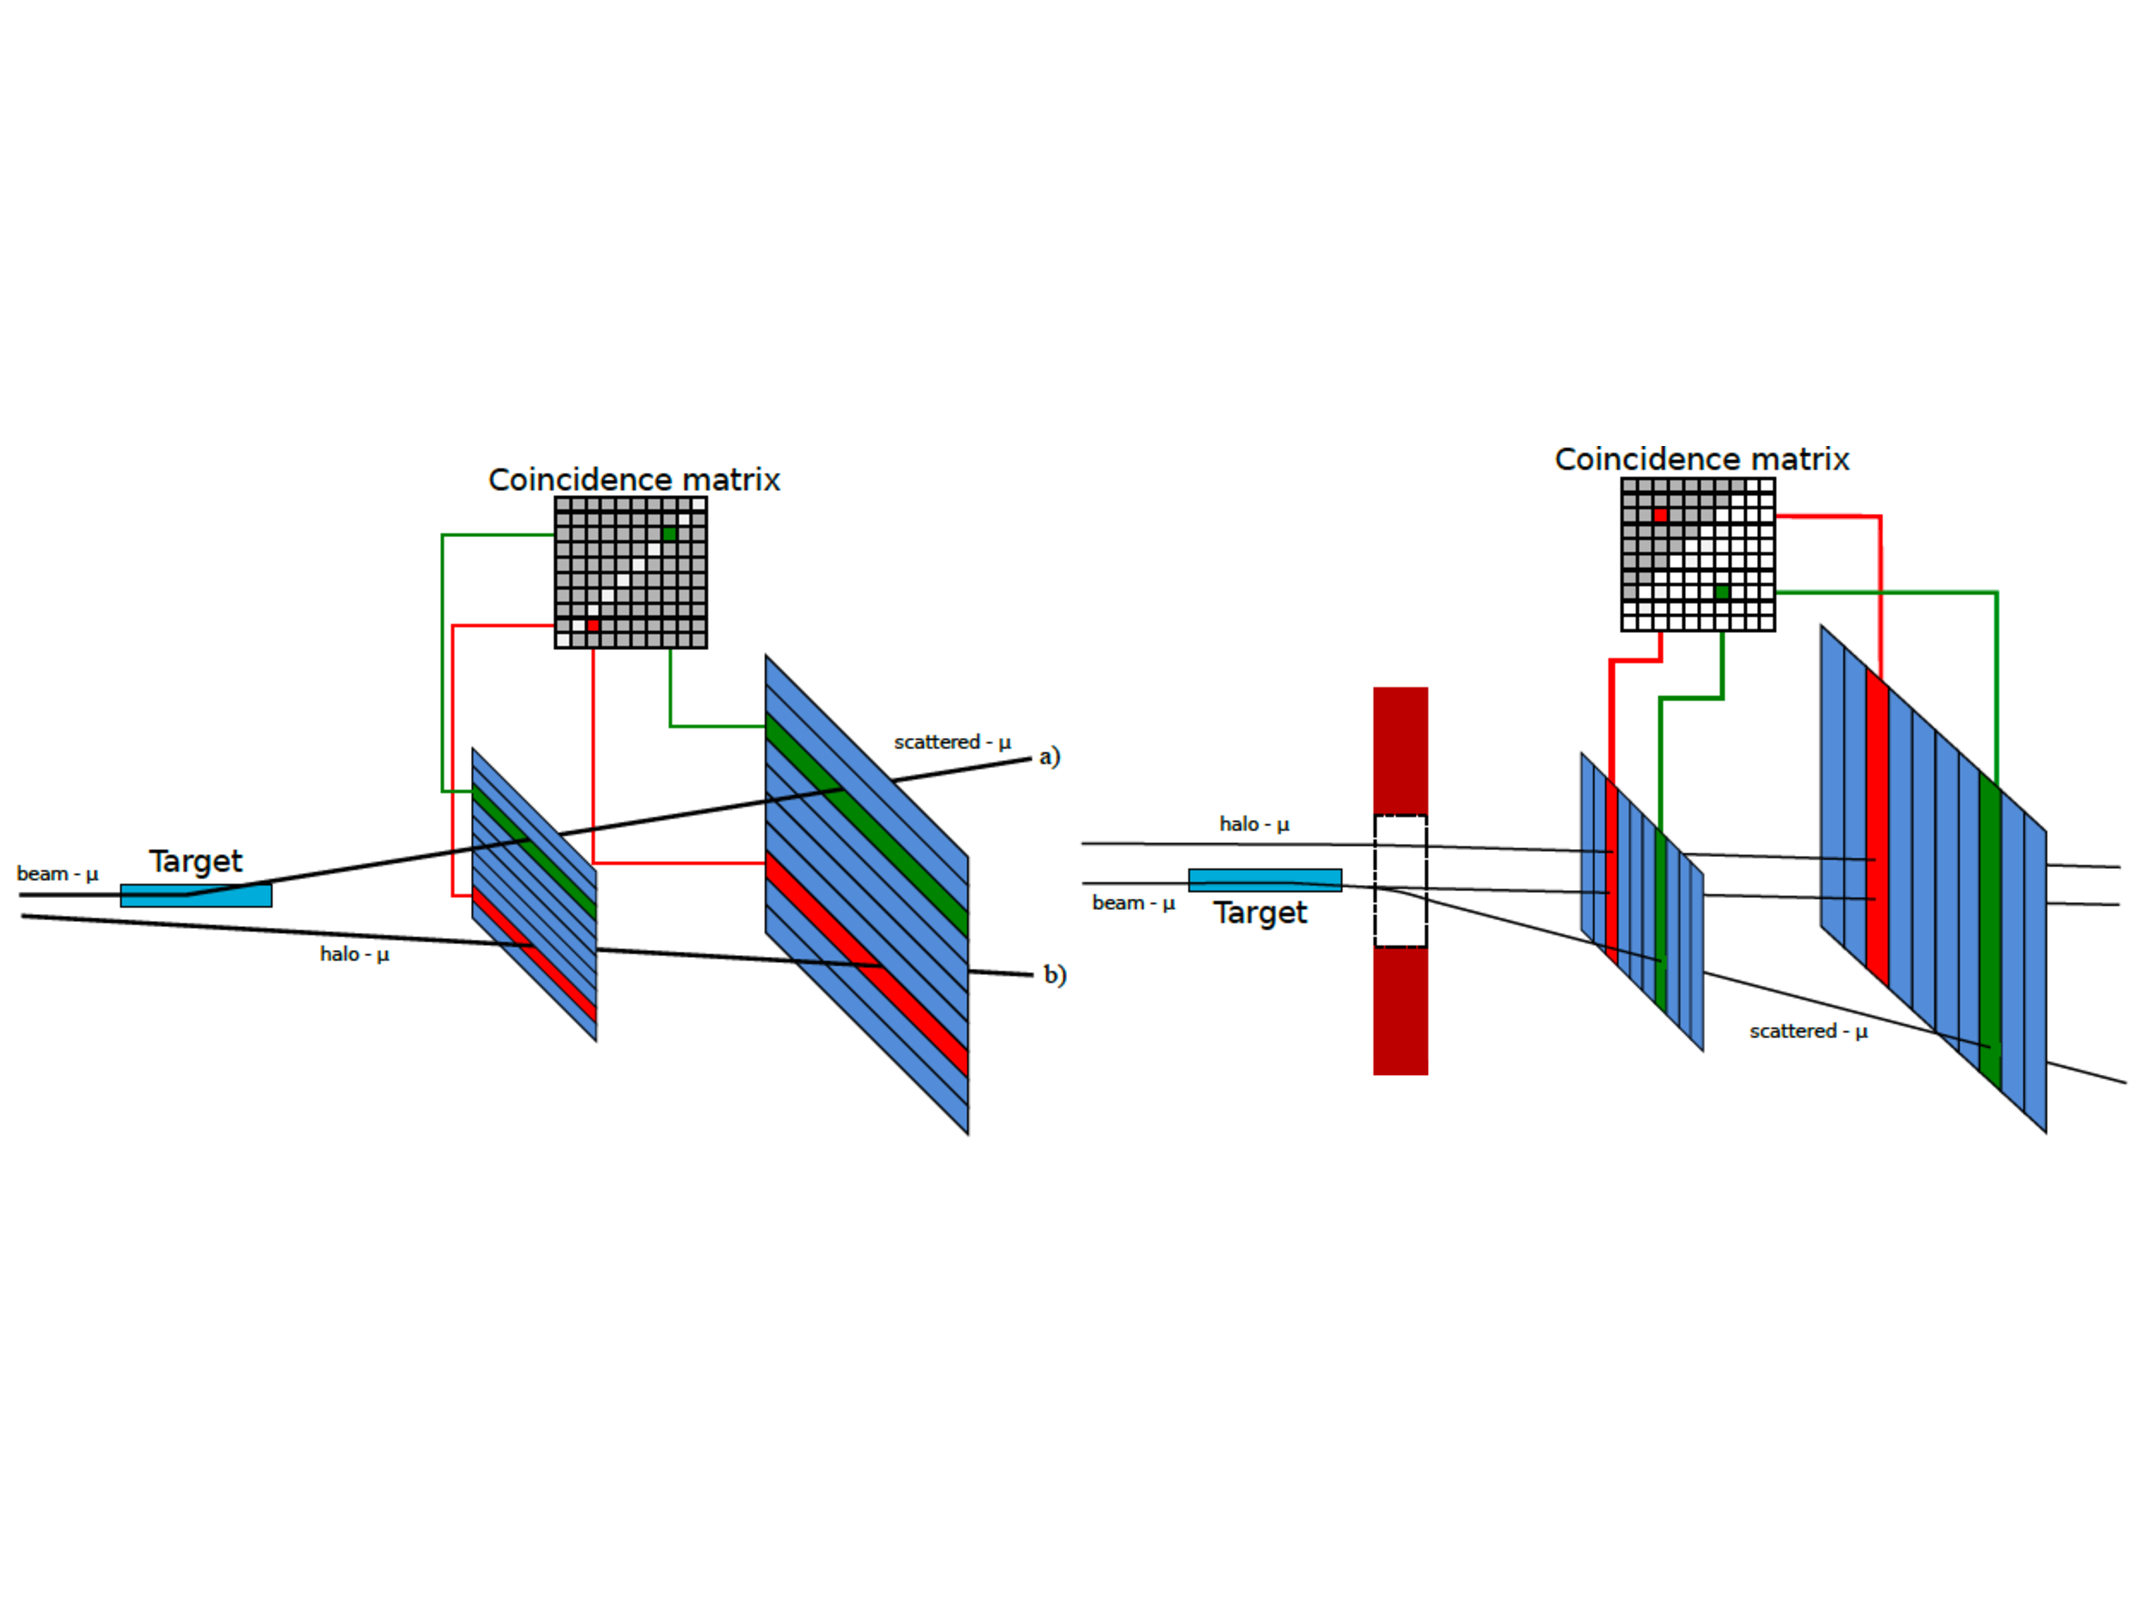
\includegraphics[width=0.9\textwidth]{TrigPrinc}
  \caption{The two types of triggers (left is target pointing and right is
    energy loss) at COMPASS and an illustration of the coincidence matrix used
    to select events of interest}
  \label{fig::TrigPrinc}
\end{figure}

\begin{figure}[h!t]
  \centering
  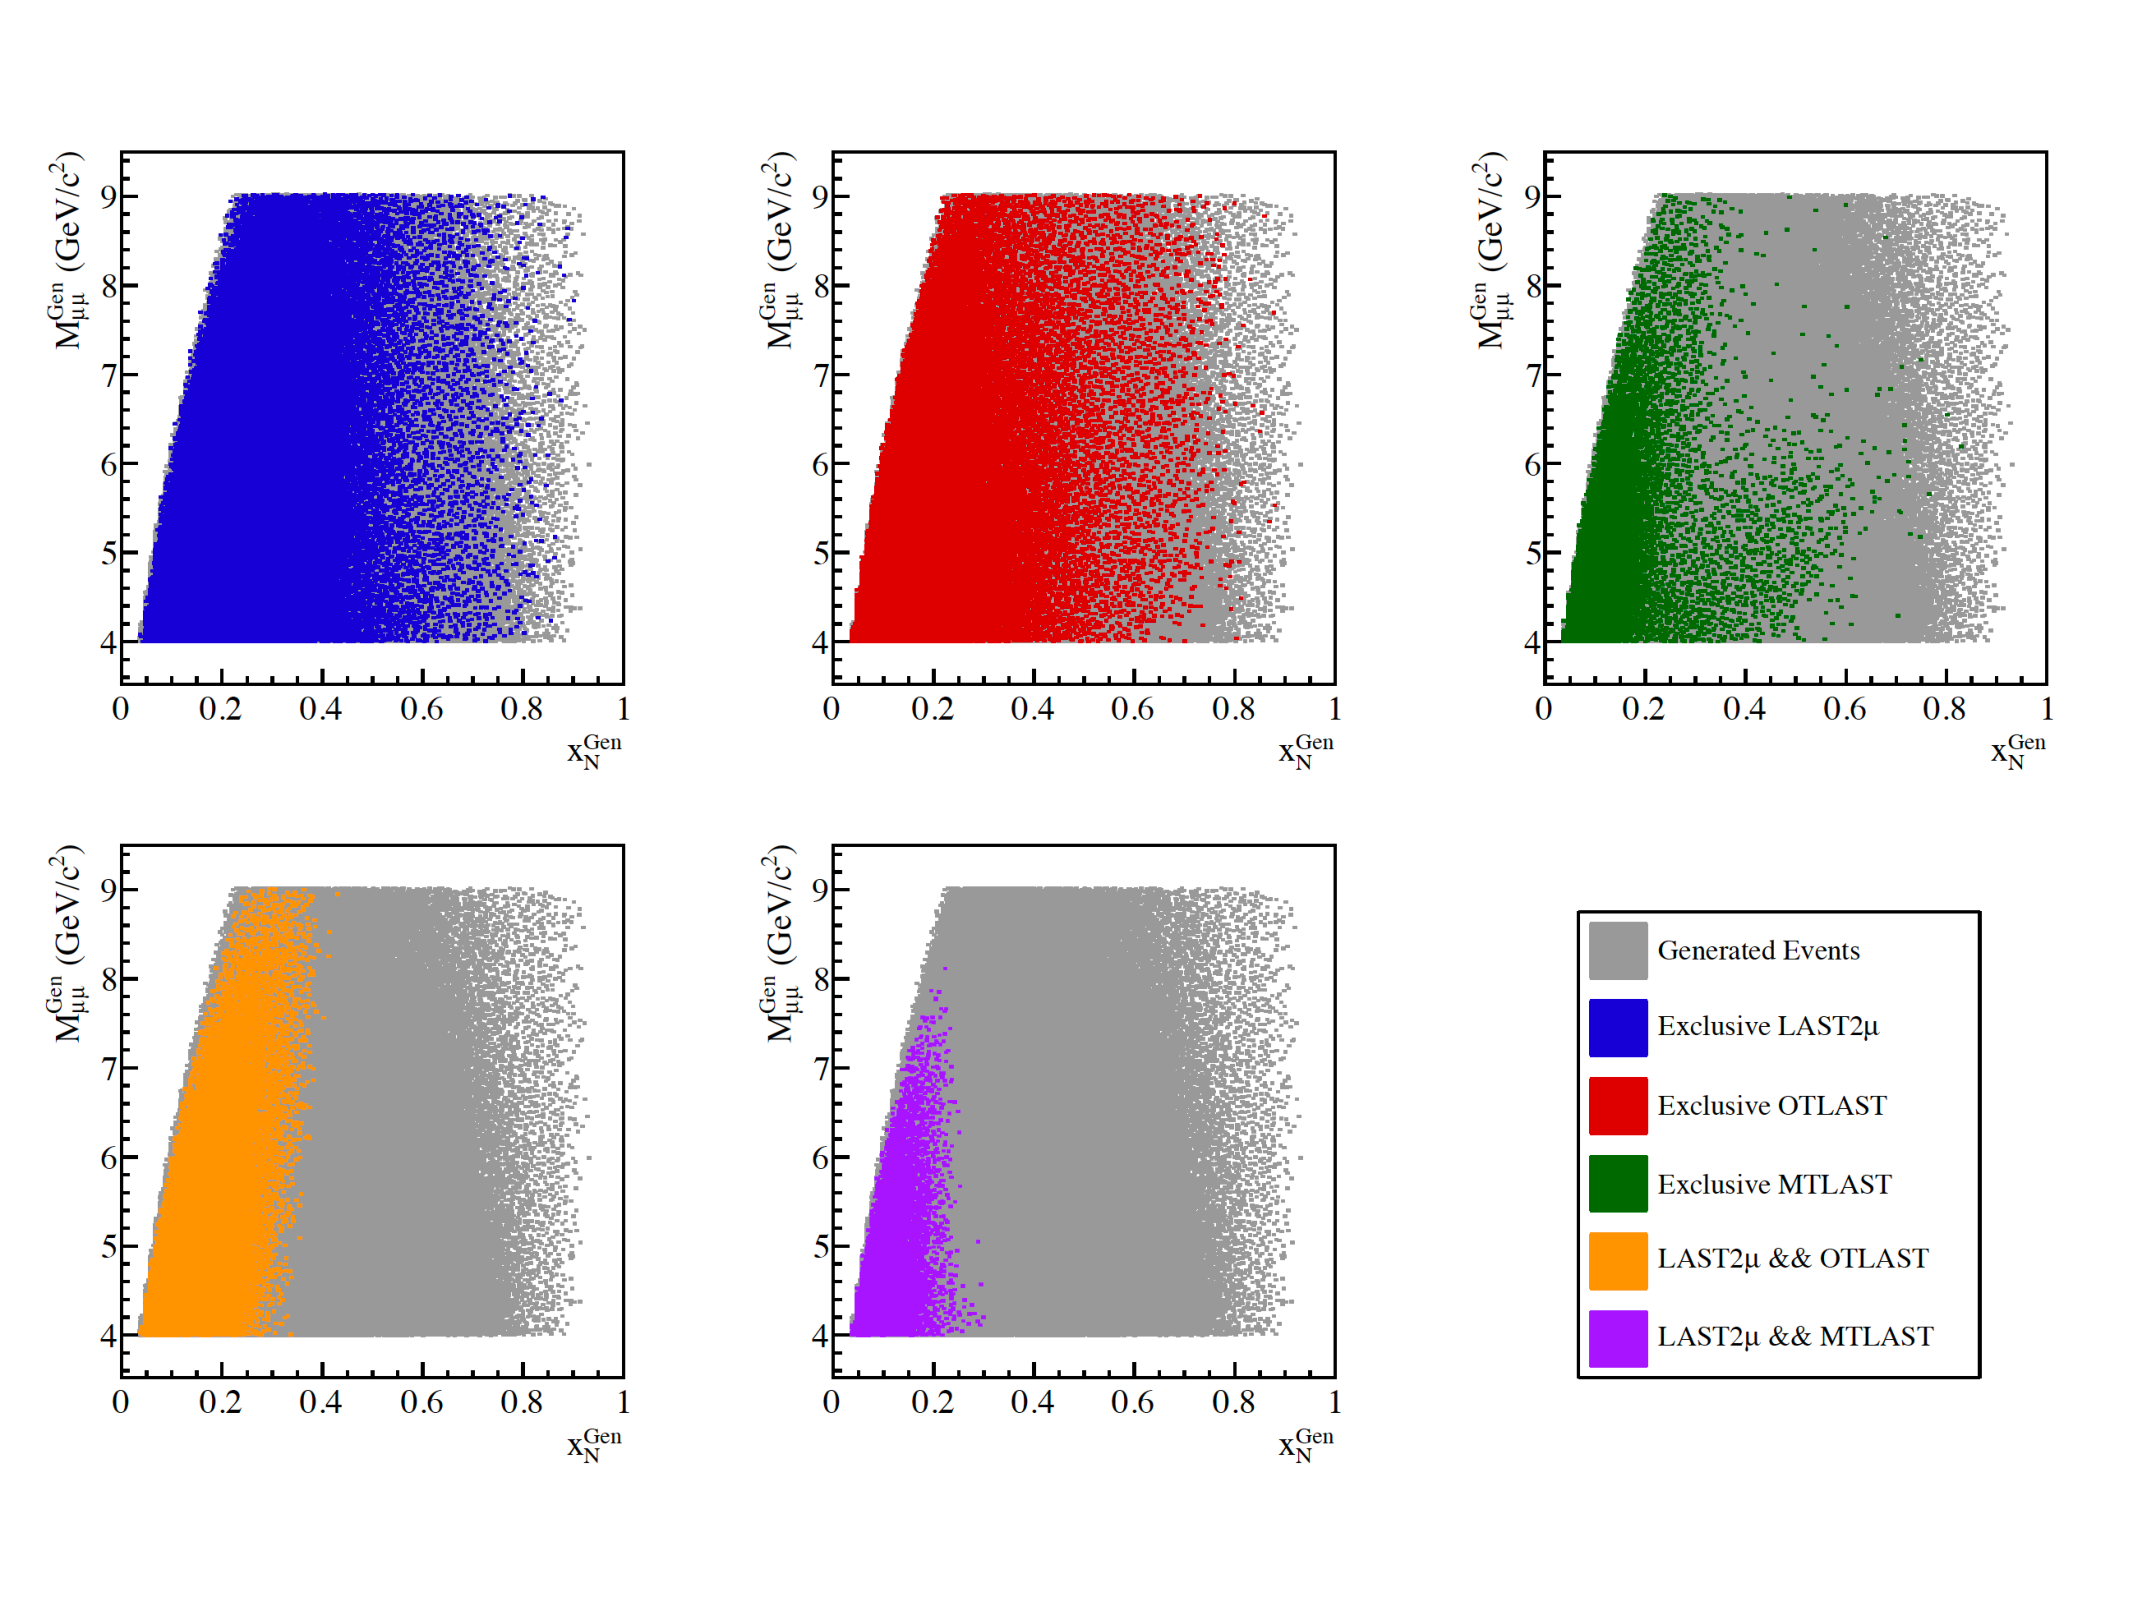
\includegraphics[width=0.9\textwidth]{TrigCov6}
  \caption{The kinematic coverage for the 2015 triggers determined from
    Monte-Carlo studies}
  \label{fig::TrigCov6}
\end{figure}

In addition to signaling when interesting events occur, it is also import to
signal when background events are occurring.  For this reason there is also a
veto system upstream of the target as shown in Fig.~\ref{fig::TriggerElements}.
This veto trigger consist of hodoscopes attached to PMTs as well.  It is
centered on the beam axis but has hole center on the nominal beam line.  The
veto trigger is used to reject halo muons which surround the beam.  Halo muons
result from the beam decaying, as in Eq.~\ref{eqn::pionDecay} and
Eq.~\ref{eqn::kaonDecay}, where this decay occurs upstream of the target but
downstream of the ABS absorbers.  The muon halo surrounds the hadron beam due to
the muon's lower momentum, and it is for this reason that the veto hodoscopes,
outside of the beam line, are able to reject events that would occur due to the
halo.

There is one trigger in the spectrometer hall that is not a hodoscopes.  This is
the calorimeter trigger (CT).  The CT can be used as a trigger when a particle
deposits more than a certain energy threshold in the specified calorimeter.  In
2015 this trigger was only used as an independent study of the other triggers at
COMPASS. Particularly the CT was used to measure the trigger hodoscopes
efficiencies. \par

The last trigger used at COMPASS is a random trigger.  This trigger is setup
outside of the spectrometer area and registers a signal when a radioactive
source disintegrates.  In this way the random trigger is truly random.  In 2015
this trigger was used in studies of the beam flux.

In 2015, the goal was to measure two muons in the spectrometer.  For this
reason, two triggers must each signal a particle in coincidence for an event to
be registered.  For physics analysis the coincidence triggers are either two
muons in LAS (LASxLAS), one muon in LAS and one in the OT (LASxOT) or one muon
in LAS and one muon in the MT (LASxMT).  The LASxLAS trigger system covers the
high Q$^2$ and high x$_{\mathrm{beam}}$ phase space whereas the triggers
including a SAS hodoscope cover lower Q$^2$ values.  In addition to these three
dimuon triggers where three single muon triggers corresponding to a particle in
LAS, MT or OT.  These three signle muon triggers, however, where pre-scaled down
to only take every 500, 100 or 100 events respectively.  For further tests 2015
included a random trigger and a beam trigger pre-scaled down by 35000.


\section{Data Acquisition}
The data acquisition (DAQ) collects data from the over 250,000 detector channels
and transfers this data to storage on magnetic tape at CASTOR (CERN Advanced
STORage).  Despite the triggering system used to reduce the data rate, the data
still is recorded at event rates between 10~kHz to 100~kHz.  A typical COMPASS
event size is 45~kB.  The DAQ is designed to process these data rates and size
while minimizing the dead time associated with data collection and transfer. In
2015 the dead time was approximately 10\%.  The total data the DAQ recorded,
after the spectrometer finished commissioning, was approximately 750~terabytes
of raw data. \par

Data collection begins with the digitization of information from a detector
channel.  This digitization is performed by a time to digital converter (TDC) or
an analogue to digital converter (ADC). These TDCs and ADCs are either on the
detector FEMs or on custom COMPASS readout electronics named: GANDOALF (Generic
Advanced Numerical Device for Analog and Logic Functions), GeSiCA (Gem and
Silicon Control and Acquisition) or CATCH (COMPASS Accumulate Transfer and
Control Hardware).  After digitization the data is transferred by optical fibers
to an FPGA multiplexer where the data is buffered by spill and arranged by
event.  From there an FPGA switch sends the data to multiplexer slaves.  The
slaves are online computers that oversee the final steps for raw data and
transfer this data to CASTOR.  This whole process is shown schematically in
Fig.~\ref{fig::DAQ}.

\begin{figure}[h!t]
  \centering
  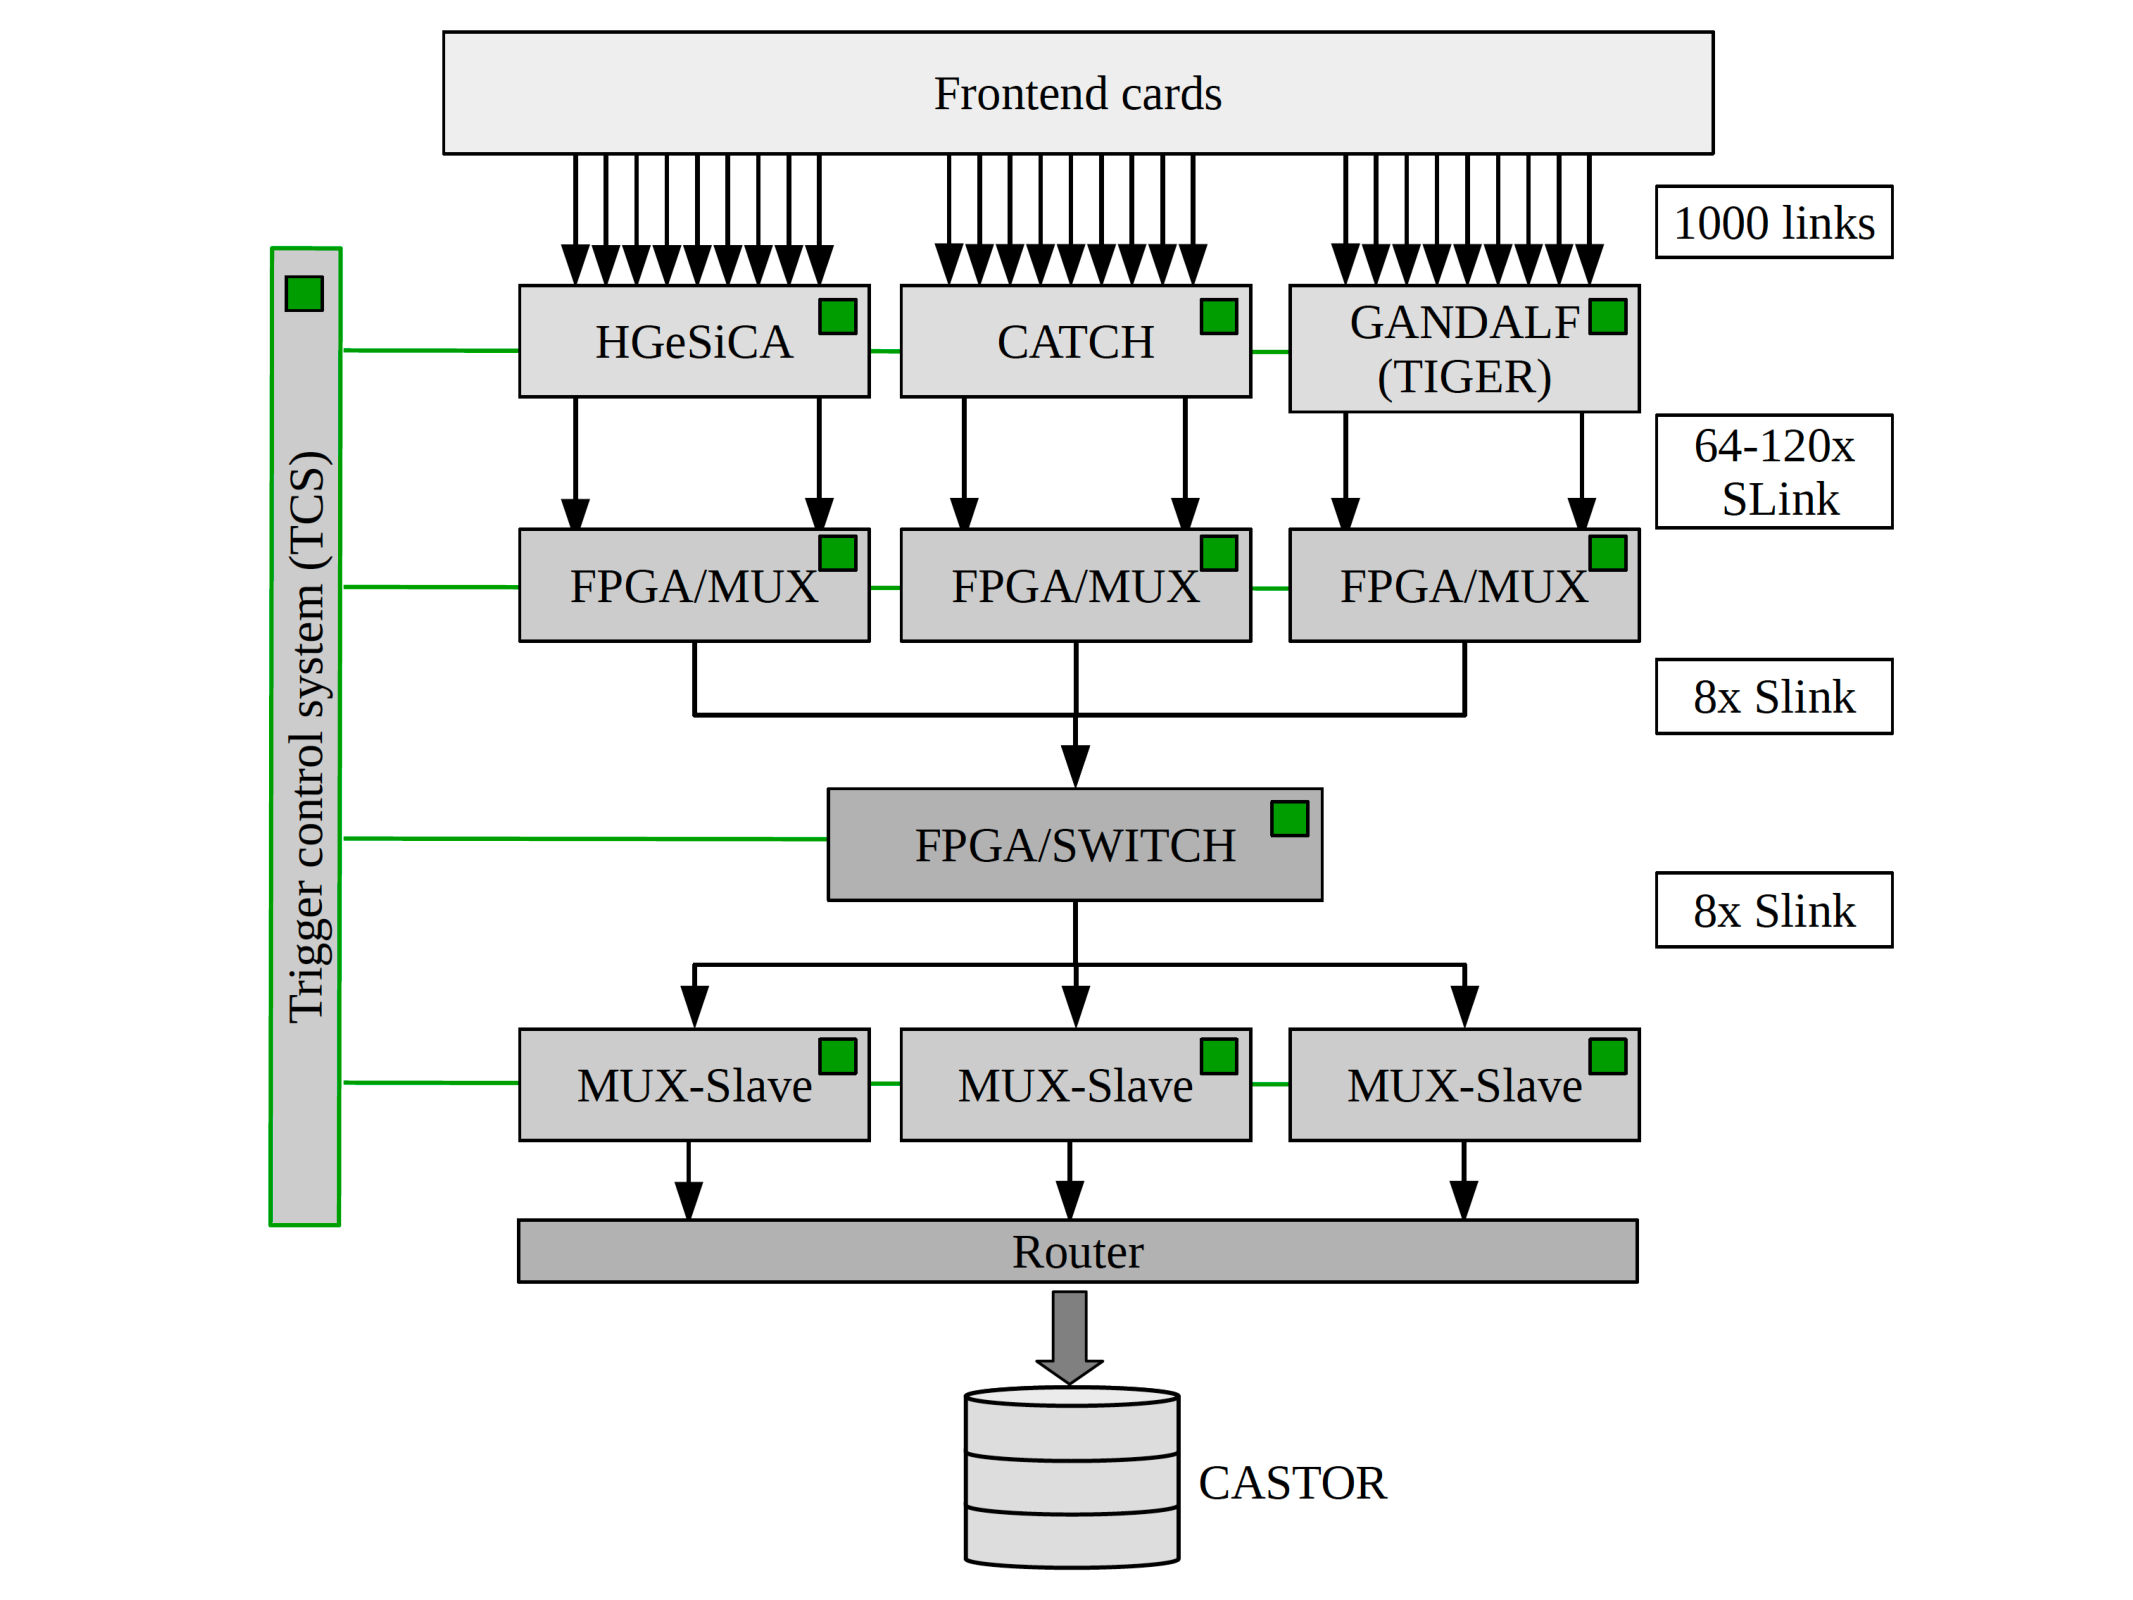
\includegraphics[width=0.6\textwidth]{DAQ}
  \caption{The data acquisition steps at COMPASS}
  \label{fig::DAQ}
\end{figure}


\section{Data Reconstruction}
The COMPASS Reconstruction and AnaLysis Program (CORAL) reconstructs the raw
data into physical quantities.  For example CORAL is able to convert the raw
data into particle tracks with momentum, charged and possibly an originating
vertex location~\cite{CORAL}.  The raw data from the DAQ is digitized timing
information from tracking detectors or digitized energy information for
calorimeters.  The process of reconstructing tracks takes the detector timing
information and determines a position in space for a particular tracking
detector based on a calibration.  CORAL then uses a Kalman Filter to determine
straight tracks in regions with no or low magnetic field~\cite{KalmanFilter}.
The tracks are then connected through the magnetic field using a fast lookup
table for known possible bending radii.  At this point a track is determined to
have a momentum, charge and a $\chi^2$ value associated with the track.  From
there the tracks are extrapolated back to the target region and the intersection
of at least two tracks is determined as a vertex.  If in addition to the two
intersecting tracks, a beam particle can be extrapolated forward to the same
vertex location then the vertex is assigned to be a primary vertex.  Otherwise
the vertex is defined as a secondary vertex.

This reconstruction stage reduces the data volume by approximately a factor of
10.  A diagram of the reconstruction data flow is shown in
Fig.~\ref{fig::CORAL}.  In 2015 there were several data reconstructions
performed.  Between each reconstruction improvements were made to detector
calibrations, detector alignment, beam tracking and any other preprocessing
improvements that could be made.  The final two productions are the t3
production and the slot1 production.  The results shown in this thesis are from
either t3 or slot1 productions.\par

\begin{figure}[h!t]
  \centering
  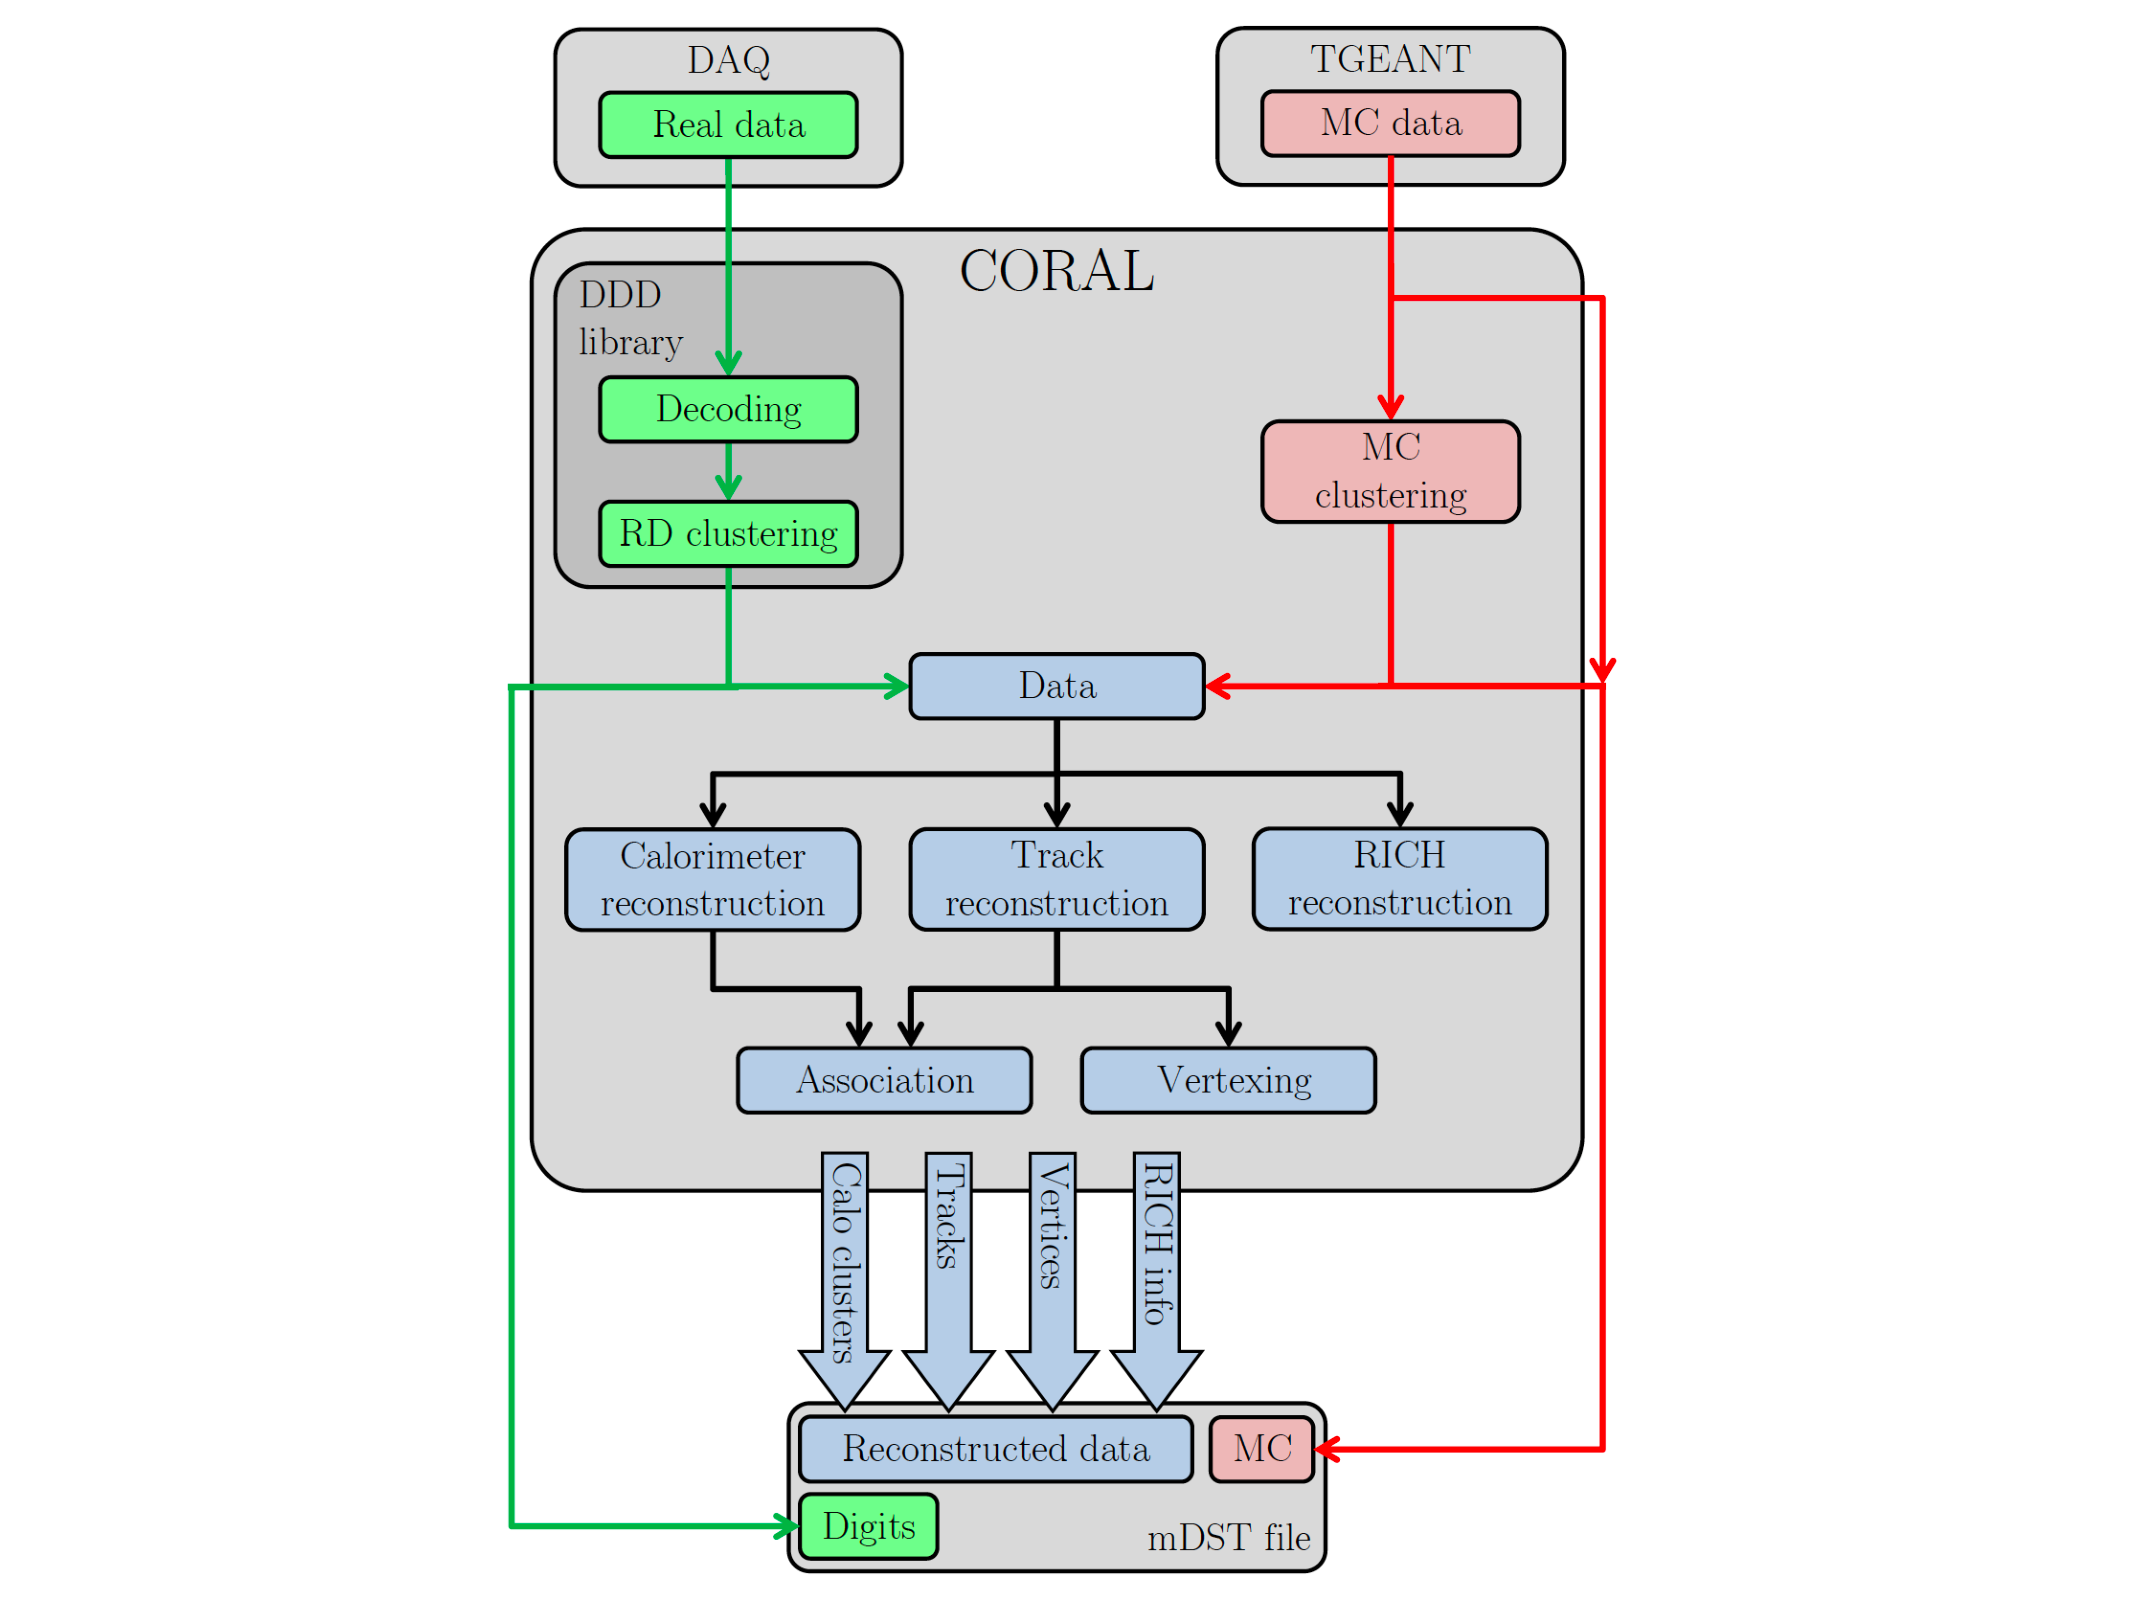
\includegraphics[width=0.6\textwidth]{CORAL}
  \caption{The schematic of the CORAL reconstruction process}
  \label{fig::CORAL}
\end{figure}

Once reconstruction has been performed the data is stored in data structured
trees (DSTs).  The usual procedure of reconstruction which gives physical values
such as momentum and charge to tracks, results in data called miniDSTs.  There
is also the possibility to save more information, for example detector hit
location information, to make so called fatDSTs.  These DSTs are now in a format
which can be processed by PHAST (PHysics Analysis Software Tool).  PHAST is a
COMPASS program written to further analyze physics data.  With PHAST there is
the possibility to loop over all the miniDSTs and make certain cuts and to
produce a so called $\mu$DSTs based on these cuts.  In 2015 $\mu$DSTs were made
for all the analysis data where a cut was applied to the miniDSTs saving only
events with at least two muons.  Both CORAL and PHAST are fully object-oriented
C++ programs. \par

\subsection{Monte-Carlo Production}
Monte-Carlo data is simulated data which is performed in three steps.  First a
programs generates specific physics processes based on their theoretical
probabilities.  The generators of Monte-Carlo used for this thesis are PYTHIA
versions 6 and 8~\cite{pythia}.  Next a GEANT4 simulation of COMPASS determines
if a detector will register a hit from these generated physics processes.  This
saves the data in a raw data format which can be reconstructed by CORAL.
Finally the simulated data is reconstructed by CORAL and analyzed in PHAST the
same as if the data were real data. \par


\section{2015 Drell-Yan Data Taking}
The 2015 Drell-Yan data taking is one of the main programs for the COMPASS-II
experiment.  The data taking began in April of 2015 and ended in November of
that year.  The physics data used for analysis started in July and finished at
the end of data taking.  The data recorded before July was used for calibrations
and commissioning.  The total analysis data was split into nine data periods
labeled W07-W15 where each data period corresponded to approximately two weeks
of beam time. The spin orientation of each target cell was reversed after the
first week of every period to reduce systematic effects arising from different
geometric acceptances and luminosities of the up and downstream target
cells. \par

\subsection{Hadron Absorber}
The previous sections in this chapter described the spectrometer setup generally
and mentioned the specifics for the 2015 setup.  The main unique hardware
addition in 2015 is the hadron absorber.  The hadron absorber was installed
because the beam intensity is high and results in many main strong interactions
in the target.  For this reason the first tracking detectors upstream of SM1
have occupancies which are too high for tracking.  Therefore the hadron absorber
was installed to prevent all particles except muons from entering the
spectometer. \par

The hadron absorber was placed just downstream of the two target cells as can be
seen in Fig.~\ref{fig::Habs}.  The absorber corresponded to approximately 7.5
interactions lengths of material where the material was mostly alumina
(Al$_2$O$_3$) and concrete.  Inside the absorber was an aluminum target followed
by a tungsten plug, each of radius 2.5 cm.  The tungsten was used as a beam dump
while the aluminum was present to prevent back scattering from the tungsten beam
plug.  A side view showing the dimensions and materials used can be seen in
Fig.~\ref{fig::Abside}.  Both the aluminum target and tungsten plug served the
double purposes as absorbers and also as unpolarized nuclear targets.  In
addition to the hadron absorber two thin $^6\mathrm{Li}$ absorbers were added
just downstream of the primary absorber to absorb thermal neutrons produced in
the primary absorber.  This $^6\mathrm{Li}$ absorber was proposed to improve the
performance of the first tracking detector downstream of the target even with
the hadron absorber installed. \par

\begin{figure}[h!t]
  \centering
  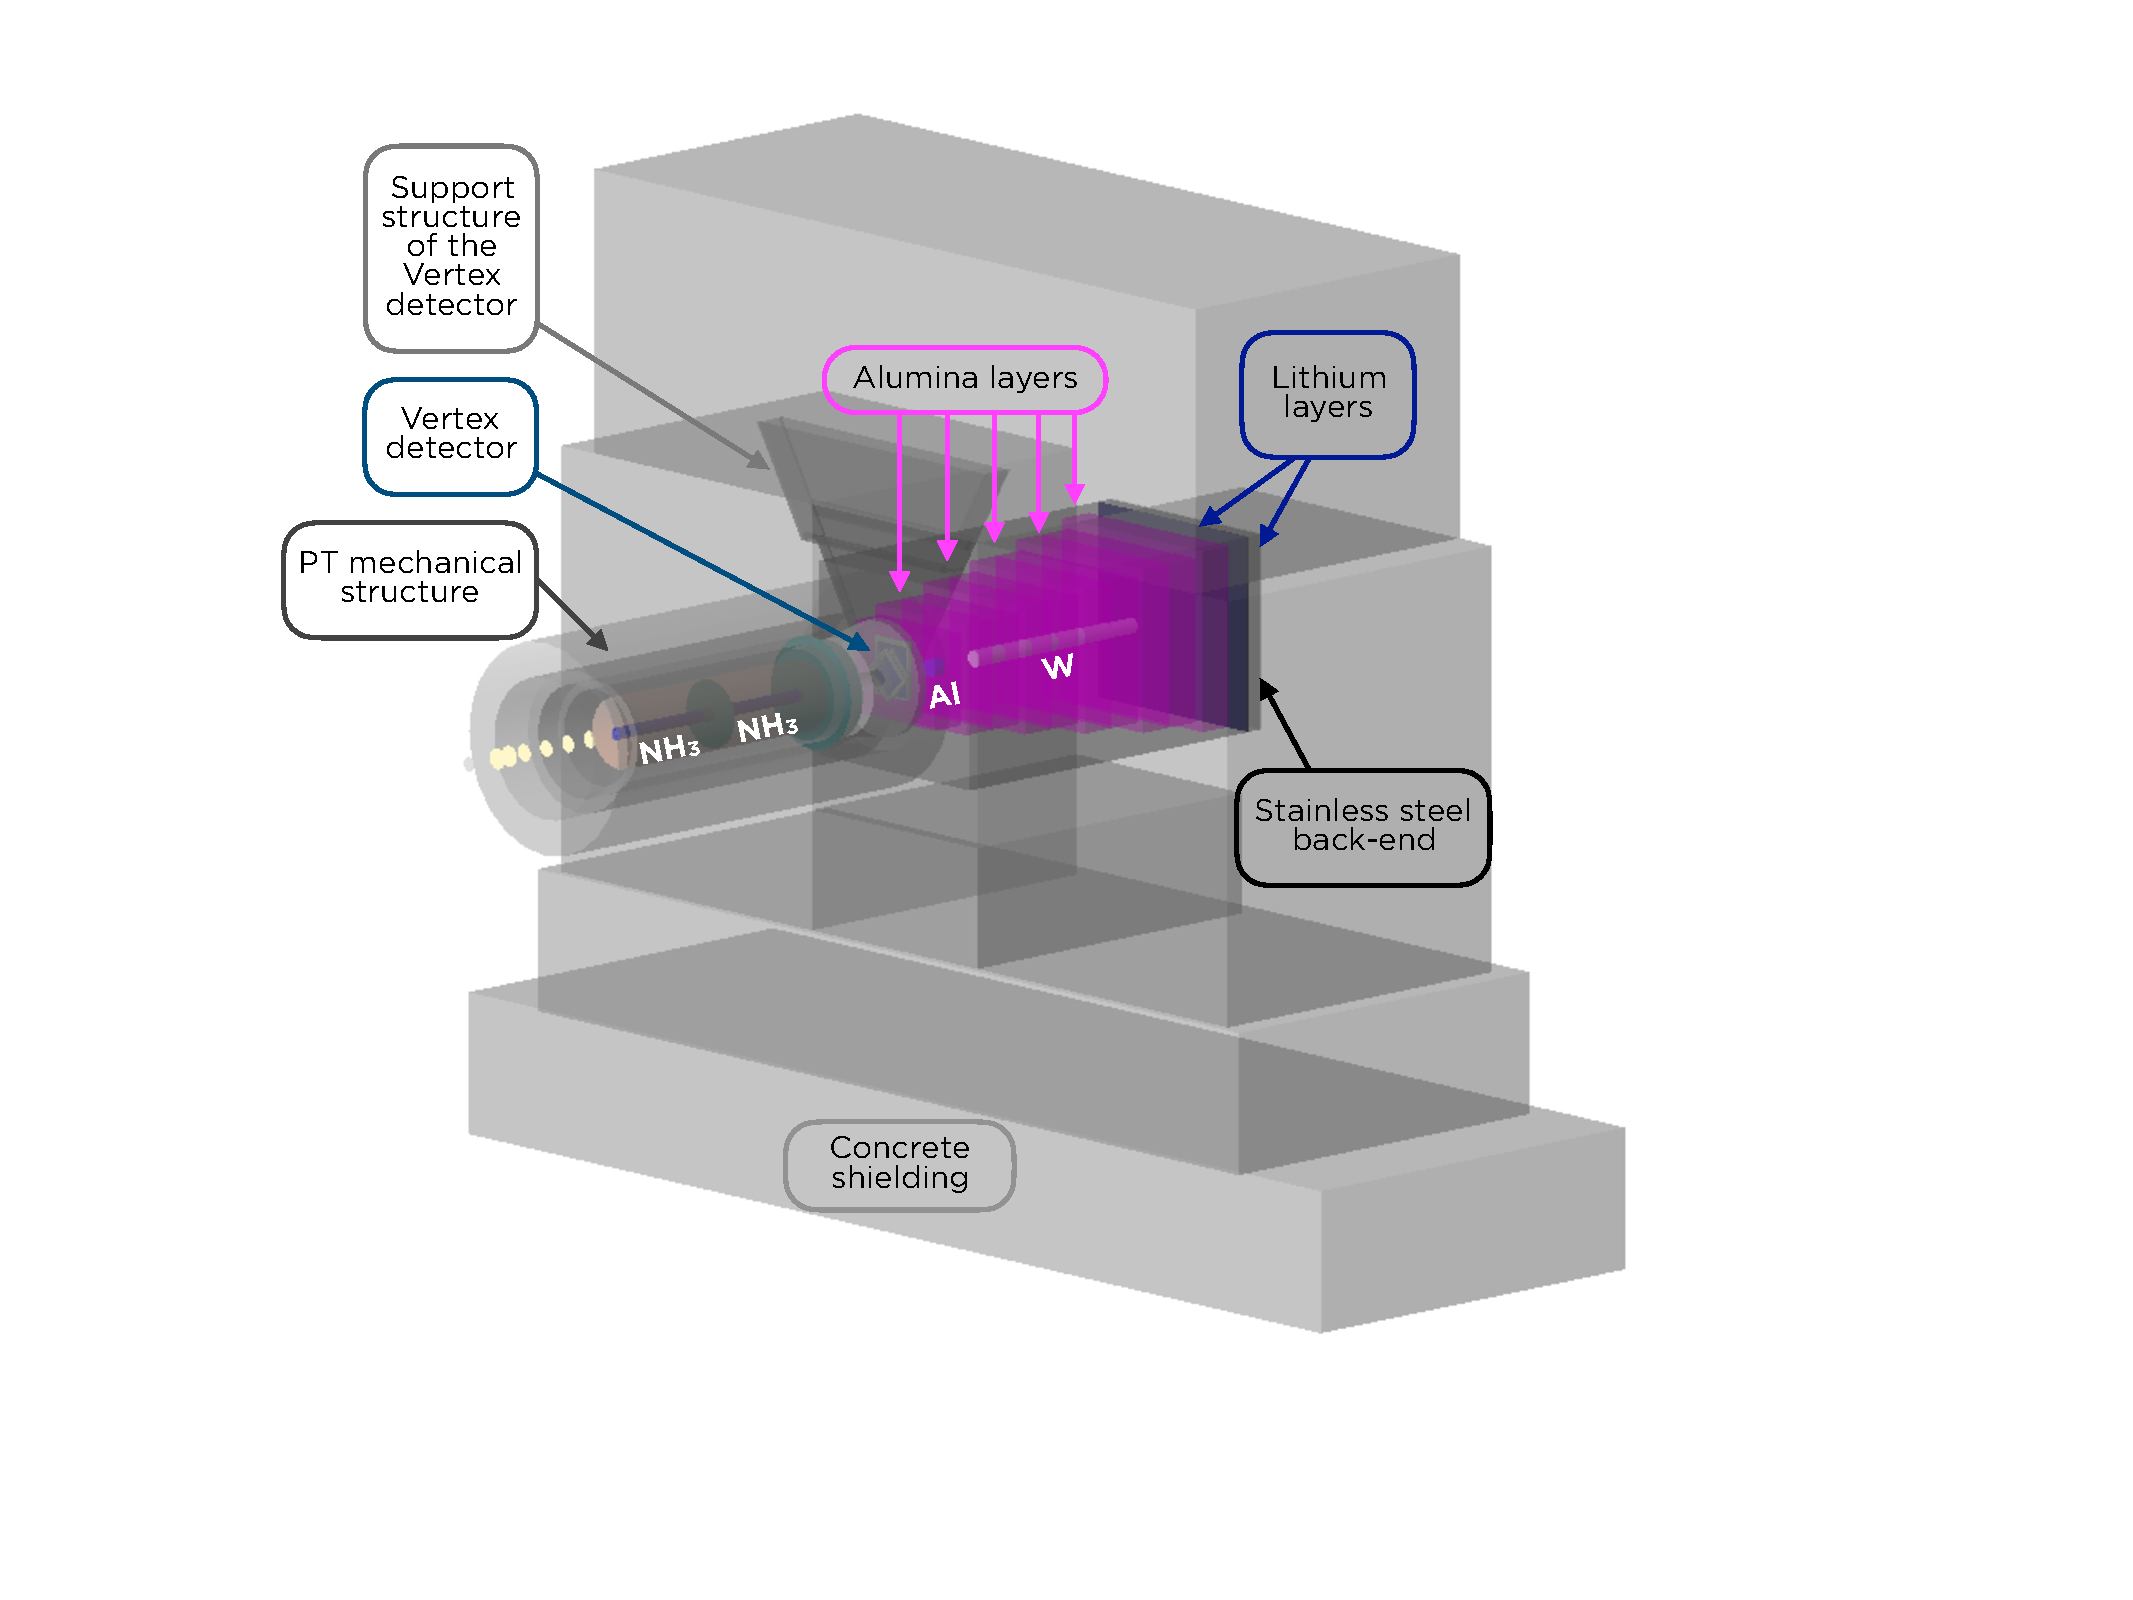
\includegraphics[width=0.6\textwidth]{Habs}
  \caption{The hadron absorber downstream of the polarized target in 2015}
  \label{fig::Habs}
\end{figure}

\begin{figure}[h!t]
  \centering
  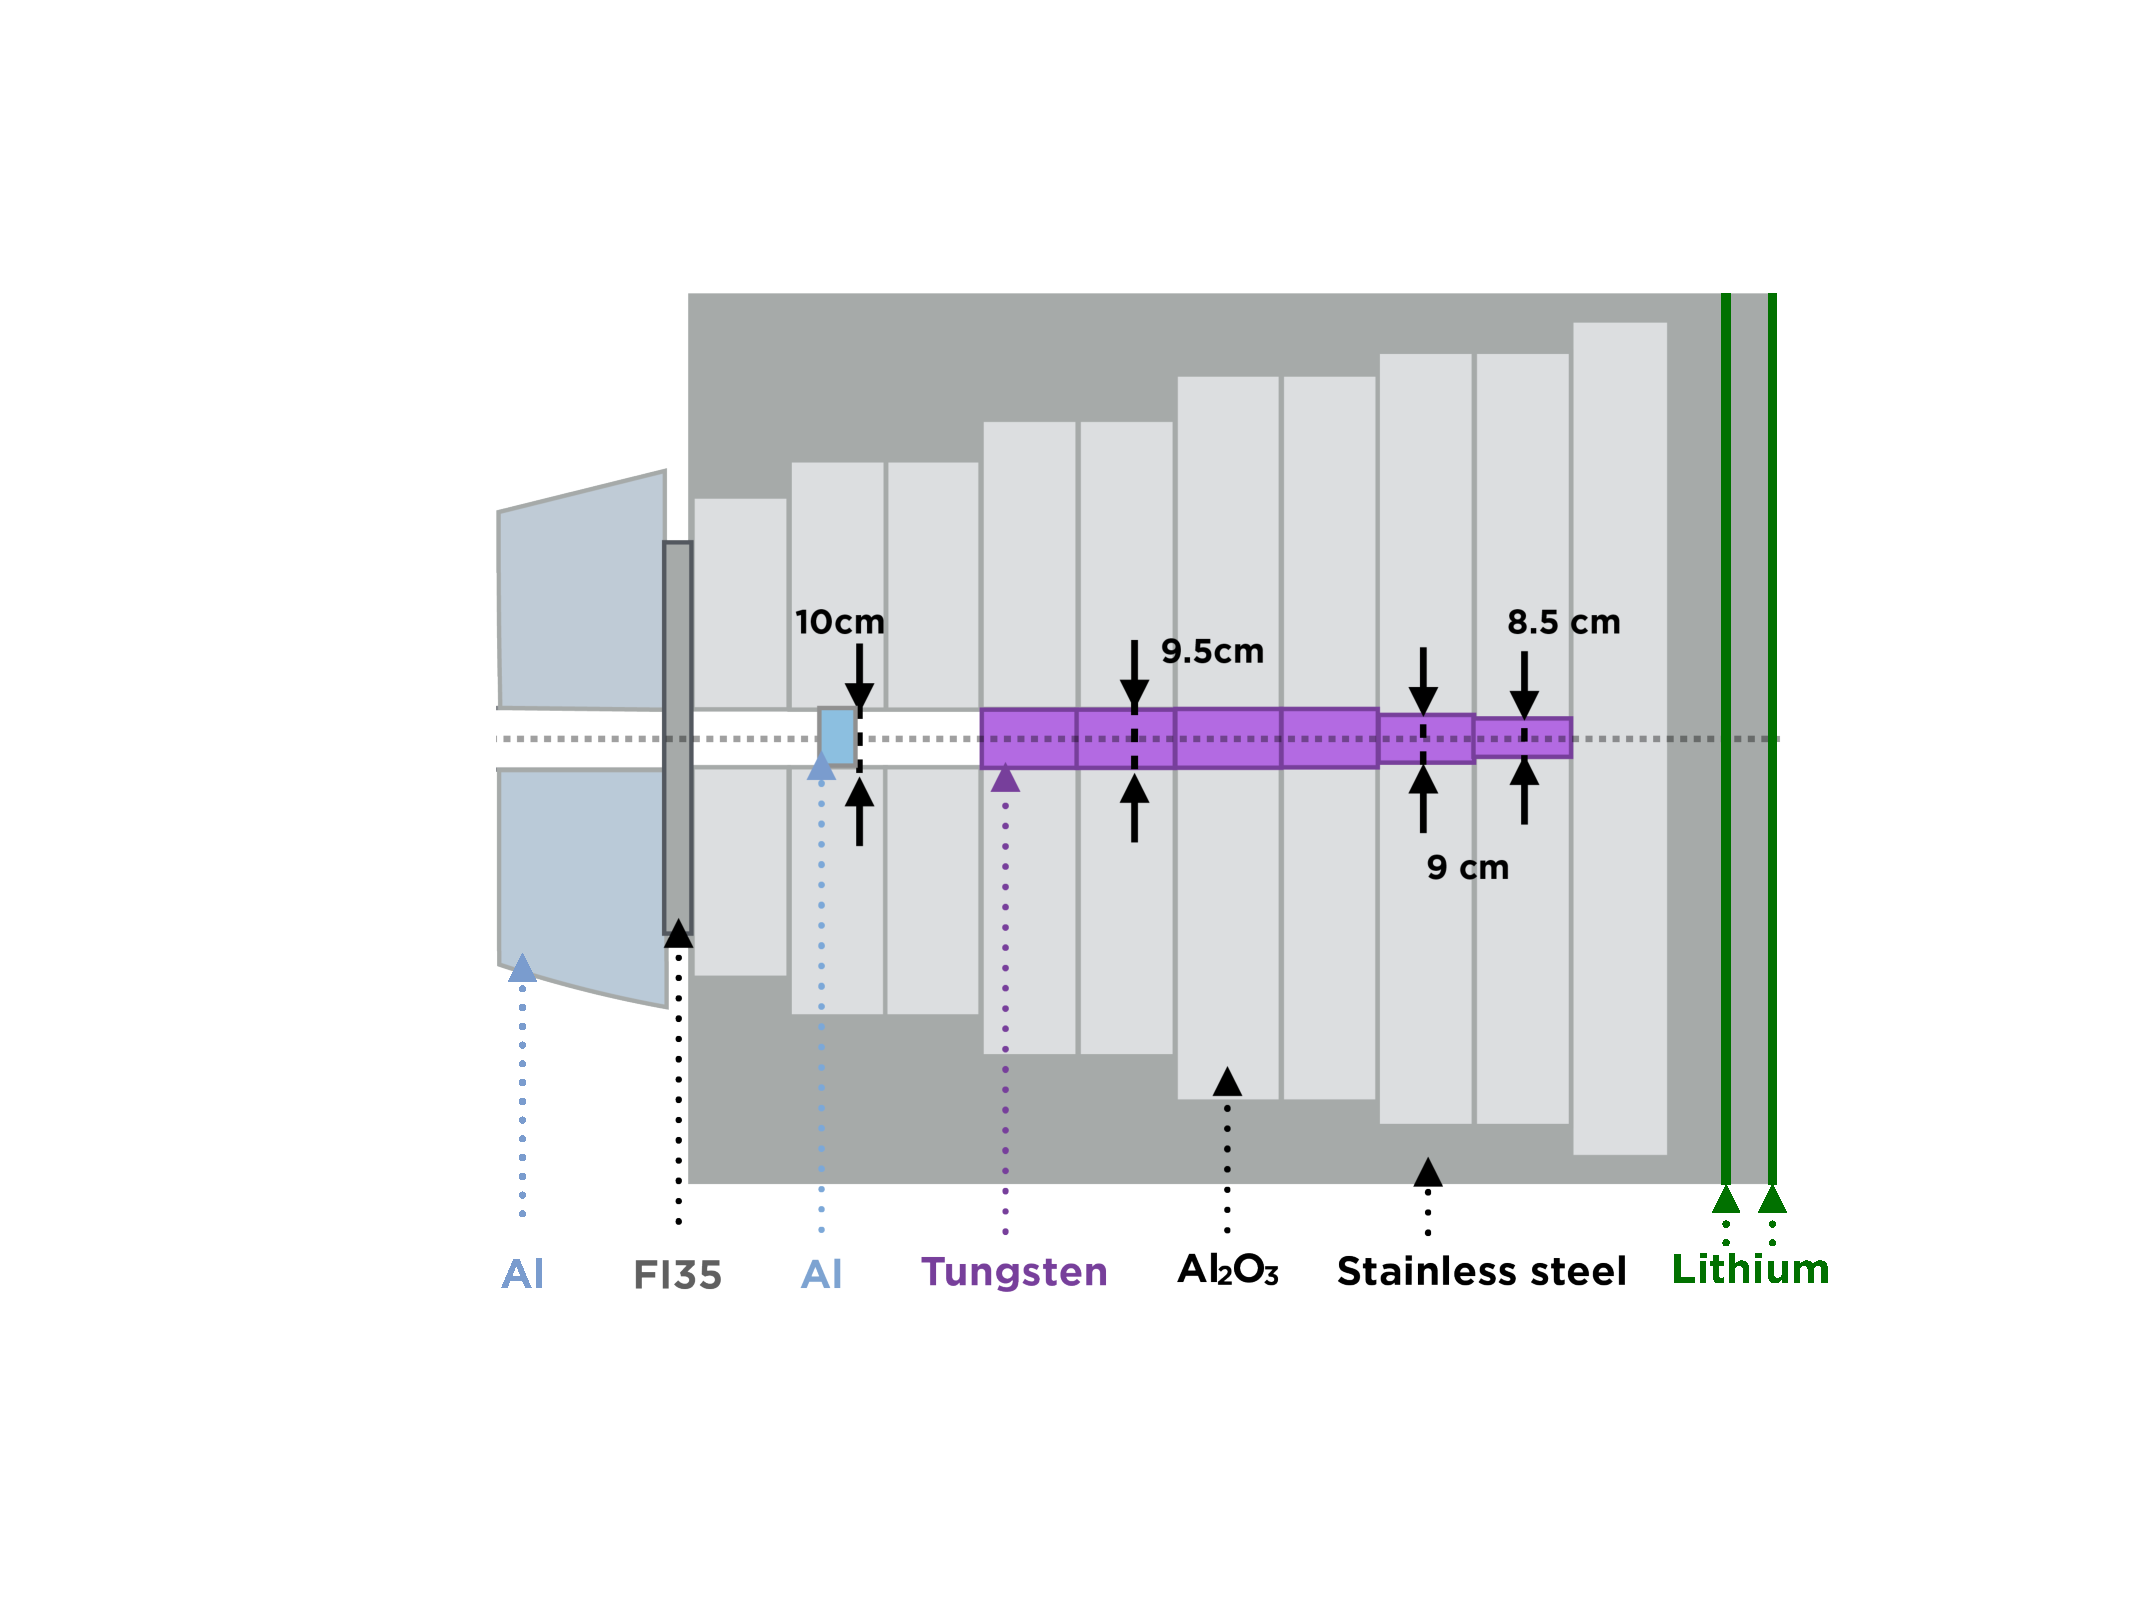
\includegraphics[width=0.6\textwidth]{Abside}
  \caption{Side view of the hadron absorber used in 2015}
  \label{fig::Abside}
\end{figure}
